% future/future.tex
% SPDX-License-Identifier: CC-BY-SA-3.0

\QuickQuizChapter{chp:Conflicting Visions of the Future}{Conflicting Visions of the Future}
%
\Epigraph{Prediction is very difficult, especially about the future.}
	 {\emph{Niels Bohr}}

이 챕터는 병렬 프로그래밍의 미래에 대한 일부 서로 다른 전망들을 소개합니다.
이 전망들 가운데 어느것이 현실이 될지, 사실 이것들 중 하나라도 현실이 될지는
명확치가 않습니다.
그러나 이것들은 각 전망을 좋아하는 지지자들이 있기 때문에 중요하며, 충분히 많은
사람들이 무언가를 열렬하게 믿는다면, 여러분은 그 지지자들의 생각, 말, 그리고
행위에서의 영향의 형태를 통한 그 존재함의 그림자만이라도 다루게 될 겁니다.
그와는 별개로, 이 전망들 중 두개 이상의 것들이 실제 현실이 될 수도 있습니다.
하지만 대부분은 가짜입니다.
뭐가 진짜고 뭐가 가짜일지 말할 수 있다면 여러분은 부자가
될겁니다~\cite{KeithRSpitz1977}!

따라서, 뒤의 섹션들은 트랜잭셔널 메모리, 하드웨어 트랜잭셔널 메모리, 그리고
병렬 함수형 프로그래밍에 대한 개괄을 제공합니다.
하지만 먼저, 예언에 대한 경고적인 이야기를 2000년대 초로부터 가져와 봅니다.
\iffalse

This chapter presents some conflicting visions of the future of parallel
programming.
It is not clear which of these will come to pass, in fact, it is not
clear that any of them will.
They are nevertheless important because each vision has its devoted
adherents, and if enough people believe in something fervently enough,
you will need to deal with at least the shadow of that thing's existence
in the form of its
influence on the thoughts, words, and deeds of its adherents.
Besides which, it is entirely possible that one or more of these visions
will actually come to pass.
But most are bogus.
Tell which is which and you'll be rich~\cite{KeithRSpitz1977}!

Therefore, the following sections give an overview of transactional
memory, hardware transactional memory,
parallel functional programming, and quantum computing.
But first, a cautionary tale on prognostication taken from the early 2000s.
\fi

% future/cpu.tex
% SPDX-License-Identifier: CC-BY-SA-3.0

\section{The Future of CPU Technology Ain't What it Used to Be}
\label{sec:future:The Future of CPU Technology Ain't What it Used to Be}

많은 기간의 경험을 가진 렌즈를 통해 보면 과거는 항상 무척 간단하고 순수해
보입니다.
그리고 2000년대 초는 당시에는 전통적이었던, Moore's Law 가 CPU 클락 주파수의
증가를 가져오던 현상이 깨지기 시작하는 시점에 임박한, 순수했던 시대였습니다.
아, 그때도 기술의 한계에 대한 경고가 때때로 있었습니다만 그런 경고들은 수십년째
이어져 오고 있었습니다.
이를 명심한 채로, 다음의 시나리오들을 고려해 봅시다:
\iffalse

Years past always seem so simple and innocent when viewed through the
lens of many years of experience.
And the early 2000s were for the most part innocent of the impending
failure of Moore's Law to continue delivering the then-traditional
increases in CPU clock frequency.
Oh, there were the occasional warnings about the limits of technology,
but such warnings had been sounded for decades.
With that in mind, consider the following scenarios:
\fi

\begin{figure}[tb]
\centering
\resizebox{3in}{!}{
\includegraphics{cartoons/r-2014-CPU-future-uniprocessor-uber-alles}}
\caption{Uniprocessor \"Uber Alles}
\ContributedBy{Figure}{fig:future:Uniprocessor Uber Alles}{Melissa Broussard}
\end{figure}

\begin{figure}[tb]
\centering
\resizebox{3in}{!}{
\includegraphics{cartoons/r-2014-CPU-Future-Multithreaded-Mania}}
\caption{Multithreaded Mania}
\ContributedBy{Figure}{fig:future:Multithreaded Mania}{Melissa Broussard}
\end{figure}

\begin{figure}[tb]
\centering
\resizebox{3in}{!}{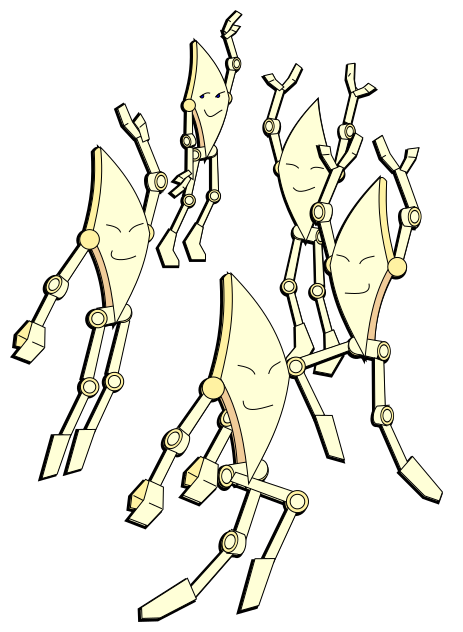
\includegraphics{cartoons/r-2014-CPU-Future-More-of-the-Same}}
\caption{More of the Same}
\ContributedBy{Figure}{fig:future:More of the Same}{Melissa Broussard}
\end{figure}

\begin{figure}[tb]
\centering
\resizebox{3in}{!}{
\includegraphics{cartoons/r-2014-CPU-Future-Crash-dummies}}
\caption{Crash Dummies Slamming into the Memory Wall}
\ContributedBy{Figure}{fig:future:Crash Dummies Slamming into the Memory Wall}{Melissa Broussard}
\end{figure}

\begin{enumerate}
\item	유니프로세서 \"Uber Alles (역주: \"Uber Alles 는 '모든것보다
	위대한' 이라는 뜻의 독일어 관용구입니다.)
	(Figure~\ref{fig:future:Uniprocessor Uber Alles}),
\item	멀티쓰레드 매니아
	(Figure~\ref{fig:future:Multithreaded Mania}),
\item	더 많은 같은것들
	(Figure~\ref{fig:future:More of the Same}), 그리고
\item	메모리 장벽에 부딪치는 것들
	(Figure~\ref{fig:future:Crash Dummies Slamming into the Memory Wall}).
\iffalse

\item	Uniprocessor \"Uber Alles
	(Figure~\ref{fig:future:Uniprocessor Uber Alles}),
\item	Multithreaded Mania
	(Figure~\ref{fig:future:Multithreaded Mania}),
\item	More of the Same
	(Figure~\ref{fig:future:More of the Same}), and
\item	Crash Dummies Slamming into the Memory Wall
	(Figure~\ref{fig:future:Crash Dummies Slamming into the Memory Wall}).
\fi
\end{enumerate}

이 각각의 시나리오를 뒤따르는 섹션들에서 다룹니다.
\iffalse

Each of these scenarios are covered in the following sections.
\fi

\subsection{Uniprocessor \"Uber Alles}
\label{sec:future:Uniprocessor Uber Alles}

2004년에 이야기 되었던 것~\cite{PaulEdwardMcKenneyPhD} 처럼:
\iffalse

As was said in 2004~\cite{PaulEdwardMcKenneyPhD}:
\fi

\begin{quote}
	이 시나리오에서, CPU 클락 속도에 있어서의 Moore's-Law 의 증가와
	수평적으로 확장되는 컴퓨팅의 계속된 발전의 조합은 SMP 시스템들을
	무의미하게 만듭니다.
	따라서 이 시나리오는 ``Uniprocessor \"Uber Alles'', 말 그대로 다른
	모든것보다 나은 유니프로세서라고 불립니다.

	이런 유니프로세서 시스템들은 인스트럭션 오버헤드만이 문제가 될텐데,
	메모리 배리어, cache thrashing, 그리고 cache contention 은 단일 CPU
	시스템에서는 문제가 없기 때문입니다.
	이 시나리오 상에서, RCU 는 NMI 들과의 상호작용과 같은 간단한 부분에서만
	유용할 것입니다.
	이미 RCU 를 구현한 운영체제는 계속 RCU 를 사용하면 되겠지만, RCU 가
	존재하지 않는 운영 체제가 RCU 를 적용해야 할지는 분명치 않습니다.

	하지만, 최근의 멀티쓰레드 CPU 의 발전은 이 시나리오가 이뤄질 가능성이
	적을 것을 시사합니다.
	\iffalse

	In this scenario, the combination of Moore's-Law increases in CPU
	clock rate and continued progress in horizontally scaled computing
	render SMP systems irrelevant.
	This scenario is therefore dubbed ``Uniprocessor \"Uber
	Alles'', literally, uniprocessors above all else.

	These uniprocessor systems would be subject only to instruction
	overhead, since memory barriers, cache thrashing, and contention
	do not affect single-CPU systems.
	In this scenario, RCU is useful only for niche applications, such
	as interacting with NMIs.
	It is not clear that an operating system lacking RCU would see
	the need to adopt it, although operating
	systems that already implement RCU might continue to do so.

	However, recent progress with multithreaded CPUs seems to indicate
	that this scenario is quite unlikely.
	\fi
\end{quote}

실제로 그렇게 되진 않을 겁니다!
하지만 한 커다란 소프트웨어 커뮤니티는 그들이 병렬성을 포용해야 한다는 사실을
받아들이기를 꺼려했는데, 이는 이 커뮤니티가 Moore's-Law 로 인한 CPU 코어 클락
주파수 상승의 ``공짜 점심'' 이 정말로 끝났다는 결론을 내리기 전이었습니다.
잊지 마세요: 믿음은 감정이므로, 이성적이고 기술적인 사고 과정의 결과가 아닐 수
있습니다!
\iffalse

Unlikely indeed!
But the larger software community was reluctant to accept the fact that
they would need to embrace parallelism, and so it was some time before
this community concluded that the ``free lunch'' of Moore's-Law-induced
CPU core-clock frequency increases was well and truly finished.
Never forget: belief is an emotion, not necessarily the result of a
rational technical thought process!
\fi

\subsection{Multithreaded Mania}
\label{sec:future:Multithreaded Mania}

역시 2004년의 이야기~\cite{PaulEdwardMcKenneyPhD} 에서:
\iffalse

Also from 2004~\cite{PaulEdwardMcKenneyPhD}:
\fi

\begin{quote}
	Uniprocessor \"Uber Alles 의 덜 극단적인 변종은 하드웨어 멀티쓰레딩을
	제공하는 유니프로세서들을 포함하고, 멀티쓰레딩 기능을 제공하는 CPU 들은
	오늘날 많은 데스크탑과 랩탑 컴퓨터 시스템들에서 표준이 되어있습니다.
	멀티쓰레드 기능을 가장 적극적으로 제공하는 CPU 들은 모든 레벨의 캐시
	구조를 공유하고, 그로 인해 CPU 에서 CPU 로의 메모리 접근 응답시간을
	없애버려, 전통적인 동기화 메커니즘에서의 성능 페널티를 거의
	없애버립니다.
	하지만, 멀티쓰레딩 기능을 제공하는 CPU 는 메모리 배리어들로 인해
	발생하는 경쟁과 파이프라인 stall 들로 인한 오버헤드로 부담을 겪을
	겁니다.
	더 나아가서, 모든 하드웨어 쓰레드들이 모든 단계의 캐시를 공유하기
	때문에, 하나의 하드웨어 쓰레드에서 사용 가능한 캐시는 동일한 단일
	쓰레드를 사용하는 CPU 의 것의 일부분만이 될 것이어서, 많은 캐시
	사용량을 갖는 어플리케이션은 성능이 덜어질 수 있을 겁니다.
	또한, 제한된 양의 캐시만이 사용 가능하다는 점이 RCU 기반 알고리즘들을
	그것들의 grace-period 가 가져온 추가적인 메모리 사용으로 인한 성능
	페널티를 겪게 할 가능성도 있습니다.
	\iffalse

	A less-extreme variant of Uniprocessor \"Uber Alles features
	uniprocessors with hardware multithreading, and in fact
	multithreaded CPUs are now standard for many desktop and laptop
	computer systems.  The most aggressively multithreaded CPUs share
	all levels of cache hierarchy, thereby eliminating CPU-to-CPU
	memory latency, in turn greatly reducing the performance
	penalty for traditional synchronization mechanisms.  However,
	a multithreaded CPU would still incur overhead due to contention
	and to pipeline stalls caused by memory barriers.  Furthermore,
	because all hardware threads share all levels of cache, the
	cache available to a given hardware thread is a fraction of
	what it would be on an equivalent single-threaded CPU, which can
	degrade performance for applications with large cache footprints.
	There is also some possibility that the restricted amount of cache
	available will cause RCU-based algorithms to incur performance
	penalties due to their grace-period-induced additional memory
	consumption.  Investigating this possibility is future work.
	\fi

	하지만, 그런 성능 저하를 막기 위해서는, 멀티쓰레드 기능을 제공하는 CPU
	들과 multi-CPU 칩들이 적어도 하드웨어 쓰레드별 기본 위에서 캐시의 어느
	단계에서는 파티션을 가져야 합니다.
	이는 각각의 하드웨어 쓰레드가 사용 가능한 캐시의 양은 증가시킵니다만,
	다시 하나의 하드웨어 쓰레드에서 다른 쓰레드로 전달되는 캐시라인을 위한
	메모리 응답시간의 증가를 다시금 가져옵니다.
	\iffalse

	However, in order to avoid such performance degradation, a number
	of multithreaded CPUs and multi-CPU chips partition at least
	some of the levels of cache on a per-hardware-thread basis.
	This increases the amount of cache available to each hardware
	thread, but re-introduces memory latency for cachelines that
	are passed from one hardware thread to another.
	\fi
\end{quote}

그리고 우리 모두 이 이야기가 하나의 소켓에 꽂혀진 하나의 다이 위의 멀티쓰레드
기능을 제공하는 여러개의 코어의 형태로, 어떻게 진행되었는지 압니다.
이제 질문은 미래의 공유 메모리 시스템들은 하나의 소켓에 들어맞을 것인지가
됩니다.
\iffalse

And we all know how this story has played out, with multiple multi-threaded
cores on a single die plugged into a single socket.
The question then becomes whether or not future shared-memory systems will
always fit into a single socket.
\fi

\subsection{More of the Same}
\label{sec:meas:More of the Same}

다시 한번 2004년의 이야기~\cite{PaulEdwardMcKenneyPhD} 로부터:
\iffalse

Again from 2004~\cite{PaulEdwardMcKenneyPhD}:
\fi

\begin{quote}
	More-of-the-Same 시나리오는 메모리 응답시간이 지금날과 거의 같은
	수준으로 머물 것이라는 가정 하에 세워집니다.

	이 시나리오는 실제로는 변화를 나타내는데, 같은 현상이 반복된다면,
	접합부의 성능이 Moore's-Law 로 인한 CPU 코어 성능의 증가에도 유지되기
	때문입니다.
	이 시나리오에서, 파이프라인 stall, 메모리 응답시간, 그리고 경쟁으로
	인한 오버헤드는 여전히 심각한 정도로 유지되고, RCU 는 오늘날 그런
	것처럼 높은 수준의 응용력을 유지하게 됩니다.
	\iffalse

	The More-of-the-Same scenario assumes that the memory-latency
	ratios will remain roughly where they are today.

	This scenario actually represents a change, since to have more
	of the same, interconnect performance must begin keeping up
	with the Moore's-Law increases in core CPU performance.  In this
	scenario, overhead due to pipeline stalls, memory latency, and
	contention remains significant, and RCU retains the high level
	of applicability that it enjoys today.
	\fi
\end{quote}

그리고 그 변화는 Moore's Law 가 여전히 제공하고 있는대로, 높아지는 수준의
집적도입니다.
하지만 더 긴 시간의 관점에서 본다면, 무엇이 될까요?
더 많은 다이당 CPU 의 갯수?
아니면 I/O, 캐시, 그리고 메모리?

서버들은 앞의 것들을 선택한 것 같고, 그사이 하나의 칩 위에 올라가는 임베디드
시스템들 (SoCs) 은 뒤의 것을 계속 선택해 갈 것 같습니다.
\iffalse

And the change has been the ever-increasing levels of integration
that Moore's Law is still providing.
But longer term, which will it be?
More CPUs per die?
Or more I/O, cache, and memory?

Servers seem to be choosing the former, while embedded systems on a chip
(SoCs) continue choosing the latter.
\fi

\subsection{Crash Dummies Slamming into the Memory Wall}
\label{sec:future:Crash Dummies Slamming into the Memory Wall}

\begin{figure}[tbp]
\centering
\epsfxsize=3in
\epsfbox{future/latencytrend}
% from Ph.D. thesis: related/latencytrend.eps
\caption{Instructions per Local Memory Reference for Sequent Computers}
\label{fig:future:Instructions per Local Memory Reference for Sequent Computers}
\end{figure}

\begin{figure}[htbp]
\centering
\epsfxsize=3in
\epsfbox{future/be-lb-n4-rf-all}
% from Ph.D. thesis: an/plots/be-lb-n4-rf-all.eps
\caption{Breakevens vs. $r$, $\lambda$ Large, Four CPUs}
\label{fig:future:Breakevens vs. r, lambda Large, Four CPUs}
\end{figure}

\begin{figure}[htbp]
\centering
\epsfxsize=3in
\epsfbox{future/be-lw-n4-rf-all}
% from Ph.D. thesis: an/plots/be-lw-n4-rf-all.eps
\caption{Breakevens vs. $r$, $\lambda$ Small, Four CPUs}
\label{fig:future:Breakevens vs. r, Worst-Case lambda, Four CPUs}
\end{figure}

그리고 2004년의 이야기~\cite{PaulEdwardMcKenneyPhD} 로부터 하나 더 인용해서:
\iffalse

And one more quote from 2004~\cite{PaulEdwardMcKenneyPhD}:
\fi

\begin{quote}
	Figure~\ref{fig:future:Instructions per Local Memory Reference for
	Sequent Computers} 에 보인 메모리 응답시간 트렌드가 계속된다면, 메모리
	응답시간은 인스트럭션 수행 오버헤드에 비해 커지기를 계속할 것입니다.
	RCU 를 많이 사용하는 리눅스와 같은 시스템들은 RCU 의 추가적인 사용이
	Figure~\ref{fig:future:Breakevens vs. r, lambda Large, Four CPUs} 에
	보인 것처럼 더 이득이 될것을 알게 될겁니다.
	이 그림에서 볼 수 있는 것처럼, RCU 가 많이 사용된다면, 증가되는 메모리
	응답시간은 RCU 에게 다른 동기화 메커니즘 대비 더 나은 이득을 주게
	될겁니다.
	반면에, RCU 를 적게 사용하는 시스템들은
	Figure~\ref{fig:future:Breakevens vs. r, Worst-Case lambda, Four CPUs}
	에 보인 것처럼 더 많은 읽기 비율을 필요로 하게 될겁니다.
	이 그림에서 볼 수 있듯이, RCU 가 적게 사용된다면, 증가되는 메모리
	응답시간 비율은 RCU 를 다른 동기화 메커니즘들 대비 단점이 많아지게
	합니다.
	리눅스는 높은 부하 아래에서 grace period 당 1,600 개가 넘는 콜백들을
	보았기 때문에, 리눅스는 앞의 카테고리에 속한다고 말하기 충분할 것
	같습니다.
	\iffalse

	If the memory-latency trends shown in
	Figure~\ref{fig:future:Instructions per Local Memory Reference for Sequent Computers}
	continue, then memory latency will continue to grow relative
	to instruction-execution overhead.
	Systems such as Linux that have significant use of RCU will find
	additional use of RCU to be profitable, as shown in
	Figure~\ref{fig:future:Breakevens vs. r, lambda Large, Four CPUs}.
	As can be seen in this figure, if RCU is heavily used, increasing
	memory-latency ratios give RCU an increasing advantage over other
	synchronization mechanisms.
	In contrast, systems with minor
	use of RCU will require increasingly high degrees of read intensity
	for use of RCU to pay off, as shown in
	Figure~\ref{fig:future:Breakevens vs. r, Worst-Case lambda, Four CPUs}.
	As can be seen in this figure, if RCU is lightly used,
	increasing memory-latency ratios
	put RCU at an increasing disadvantage compared to other synchronization
	mechanisms.
	Since Linux has been observed with over 1,600 callbacks per grace
	period under heavy load~\cite{Sarma04c},
	it seems safe to say that Linux falls into the former category.
	\fi
\end{quote}

한편, 이 구절은 RCU 가 상당한 업데이트 위주의 워크로드에서 겪을 수 있는 cache
warmth 문제를 설명하지 못하는데, 한편으로는 그런 워크로드에서 RCU 가 사용되지는
않을 것이기 때문입니다.
결과적으로, 이런 cache-warmth 문제가 문제시 되는 여러 경우에는 시퀀스 락킹이
그렇듯이 \co{SLAB_DESTROY_BY_RCU} 가 사용되도록 되었습니다.
한편으로는, 이 구절은 또한 RCU 가 스케쥴링 응답시간을 줄이거나 보안 기능을 위해
사용되지는 못할 것이란 점을 설명하지도 않습니다.

짧게 말해서, 이 챕터의 뒷부분에서 설명하는 것들을 포함해 전조들에 주의하시기
바랍니다.
\iffalse

On the one hand, this passage failed to anticipate the cache-warmth
issues that RCU can suffer from in workloads with significant update
intensity, in part because it seemed unlikely that RCU would really
be used for such workloads.
In the event, the \co{SLAB_DESTROY_BY_RCU} has been pressed into 
service in a number of instances where these cache-warmth issues would
otherwise be problematic, as has sequence locking.
On the other hand, this passage also failed to anticipate that
RCU would be used to reduce scheduling latency or for security.

In short, beware of prognostications, including those in the remainder
of this chapter.
\fi

% future/tm.tex

\section{Transactional Memory}
\label{sec:future:Transactional Memory}

데이터베이스 바깥의 영역에서 트랜잭션을 사용하자는 아이디어는 수십년 전으로
거슬러 오르는데~\cite{DBLomet1977SIGSOFT}, 이 아이디어는 데이터베이스에서와
데이터베이스 외에서의 트랜잭션에 대해 데이터베이스 외에서의 트랜잭션은
데이터베이스 트랜잭션을 정의하는 성질인 ``ACID'' 에서 ``D'' 를 빼냅니다.
하드웨어에서 메모리 기반의 트랜잭션, 또는 ``트랜잭셔널 메모리'' (TM) 을
지원하려는 아이디어는 최근의 것입니다만~\cite{Herlihy93a}, 안타깝게도 실제 많이
사용되는 하드웨어에서의 그런 트랜잭션의 지원은 그와 비슷한 것들에 대한 제안은
계속 있어왔지만~\cite{JMStone93}, 곧바로 이루어지지는 않았습니다.
그로부터 그렇게 오래지 않아, Shavit 과 Touitou 는 일반적으로 사용되는
하드웨어에서 동작할 수 있는, 메모리 접근 순서를 조정해서 소프트웨어만으로
이루어진 트랜잭셔널 메모리 구현 (STM) 을 제안했습니다.
이 제안은 여러 해동안 질질 끌려졌는데, 어쩌면 연구자 커뮤니티들의 관심은
non-blocking 동기화 (Section~\ref{sec:advsync:Non-Blocking Synchronization} 을
참고하세요) 에 열중되었기 때문일 수도 있습니다.
\iffalse

The idea of using transactions outside of databases goes back many
decades~\cite{DBLomet1977SIGSOFT}, with the key difference between
database and non-database transactions being that non-database transactions
drop the ``D'' in the ``ACID'' properties defining database transactions.
The idea of supporting memory-based transactions, or ``transactional memory''
(TM), in hardware
is more recent~\cite{Herlihy93a}, but unfortunately, support for such
transactions in commodity hardware was not immediately forthcoming,
despite other somewhat similar proposals being put forward~\cite{JMStone93}.
Not long after, Shavit and Touitou proposed a software-only implementation
of transactional memory (STM) that was capable of running on commodity
hardware, give or take memory-ordering issues.
This proposal languished for many years, perhaps due to the fact that
the research community's attention was absorbed by non-blocking
synchronization (see Section~\ref{sec:advsync:Non-Blocking Synchronization}).
\fi

하지만 세기가 변하면서, TM 은 일부 주의의 목소리를 받기
시작했고~\cite{Blundell2005DebunkTM,McKenney2007PLOSTM}, 2000년부터 2009년
사이의 중반 쯤에는 몇가지 경고의 목소리에도
불구하고~\cite{MauriceHerlihy2005-TM-manifesto.pldi,DanGrossman2007TMGCAnalogy},
그 관심의 수준이 ``열광적'' 이라 할 수 있게 되었습니다.
\iffalse

But by the turn of the century, TM started receiving
more attention~\cite{Martinez01a,Rajwar01a}, and by the middle of the
decade, the level of interest can only be termed
``incandescent''~\cite{MauriceHerlihy2005-TM-manifesto.pldi,
DanGrossman2007TMGCAnalogy}, despite a few voices of
caution~\cite{Blundell2005DebunkTM,McKenney2007PLOSTM}.
\fi

TM 에 대한 기본 아이디어는 한 섹션의 코드를 어토믹하게 수행해서 다른 쓰레드가
그 중간의 상태를 볼 수 없게 하자는 것입니다.
그렇게, TM 의 의미는 간단히 각각의 트랜잭션을 반복적으로 획득할 수 있는 글로벌
락의 획득과 해제로 감싸는 것으로, 성능과 확장성이 처참해지긴 하겠지만, 구현될
수 있습니다.
하드웨어에서든 소프트웨어에서든 TM 구현에서는 피할 수 없는 복잡성은 동시적인
트랜잭션들이 안전하게 병렬적으로 수행될 수 있는지에 대한 파악입니다.
이 파악은 동적으로 이루어지기 때문에, 충돌하는 트랜잭션들은 취소되거나
``롤백''될 수 있고, 일부 구현에서는, 이 실패한 모드가 프로그래머에게 보여질 수
있습니다.
\iffalse

The basic idea behind TM is to execute a section of
code atomically, so that other threads see no intermediate state.
As such, the semantics of TM could be implemented
by simply replacing each transaction with a recursively acquirable
global lock acquisition and release, albeit with abysmal performance
and scalability.
Much of the complexity inherent in TM implementations, whether hardware
or software, is efficiently detecting when concurrent transactions can safely
run in parallel.
Because this detection is done dynamically, conflicting transactions
can be aborted or ``rolled back'', and in some implementations, this
failure mode is visible to the programmer.
\fi

트랜잭션 롤백은 트랜잭션 크기가 줄어듦에 따라 발생률이 줄어들 것이기 때문에, TM
은 스택, 큐, 해시 테이블, 탐색 트리들과 같은 데에 사용되는 링크드 리스트 제어와
같이 작은 크기의 메모리 기반 오퍼레이션들에 매력적일 수 있습니다.
하지만, I/O 와 프로세스 생성과 같은 메모리 기반이 아닌 오퍼레이션들을 포함하는
것들과 같은, 커다란 트랜잭션들에 TM 을 적용하기는 어렵습니다.
다음 섹션들은 ``Transactional Memory
Everywhere''~\cite{PaulEMcKenney2009TMeverywhere} 의 커다란 비전을 위해
존재하는 현재의 극복해야할 사항들을 알아봅니다.
Section~\ref{sec:future:Outside World} 은 바깥의 것들과 상호동작하는 데에
나타나는 문제점들을 알아보고,
Section~\ref{sec:future:Process Modification} 는 프로세스 수정 기능들과의
상호동작을 보며,
Section~\ref{sec:future:Synchronization} 는 다른 동기화 기능들과의 상호
동작들을 살펴보며, 마지막으로
Section~\ref{sec:future:Discussion} 에서 일부 토의와 함께 마무리 합니다.
\iffalse

Because transaction roll-back is increasingly unlikely as transaction
size decreases, TM might become quite attractive for small memory-based
operations,
such as linked-list manipulations used for stacks, queues, hash tables,
and search trees.
However, it is currently much more difficult to make the case for large
transactions, particularly those containing non-memory operations such
as I/O and process creation.
The following sections look at current challenges to the grand vision of
``Transactional Memory Everywhere''~\cite{PaulEMcKenney2009TMeverywhere}.
Section~\ref{sec:future:Outside World} examines the challenges faced
interacting with the outside world,
Section~\ref{sec:future:Process Modification} looks at interactions
with process modification primitives,
Section~\ref{sec:future:Synchronization} explores interactions with
other synchronization primitives, and finally
Section~\ref{sec:future:Discussion} closes with some discussion.
\fi

\subsection{Outside World}
\label{sec:future:Outside World}

Donal Knuth 의 말을 인용하면:
\iffalse

In the words of Donald Knuth:
\fi

\begin{quote}
	많은 컴퓨터 사용자들이 입력과 출력은 ``진짜 프로그래밍'' 의 실제 부분은
	아니고, 그것들은 그저 기계로 정보를 넣고 그로부터 정보를 뽑아내기 위해
	(불행히도) 반드시 해야만 하는것들이라고 느낍니다.
	\iffalse

	Many computer users feel that input and output are not actually part
	of ``real programming,'' they are merely things that (unfortunately)
	must be done in order to get information in and out of the machine.
	\fi
\end{quote}

우리가 입력과 출력이 ``진짜 프로그래밍'' 이라 믿든 아니라 믿든, 대부분의 컴퓨터
시스템들에 있어서, 바깥 세상과의 상호작용이 첫번째 중요도의 요구사항임은
사실입니다.
따라서 이 섹션은 트랜잭셔널의, I/O 오퍼레이션을 통해서든, 시간 딜레이를
통해서든, 또는 영구적 저장장치를 이용해서든 이루어지는, 상호작용을 위한
기능들에 대해 비평해 봅니다.
\iffalse

Whether we believe that input and output are ``real programming'' or
not, the fact is that for most computer systems, interaction with the
outside world is a first-class requirement.
This section therefore critiques transactional memory's ability to
so interact, whether via I/O operations, time delays, or persistent
storage.
\fi

\subsubsection{I/O Operations}
\label{sec:future:I/O Operations}

누군가는 I/O 오퍼레이션을 락 기반의 크리티컬 섹션 안에서 할수도, 적어도
원칙적으로는, RCU read-side 크리티컬 섹션 안에서 할수도 있습니다.
트랜잭션 안에서 I/O 오퍼레이션을 수행하려 하면 어떻게 될까요?
\iffalse

One can execute I/O operations within a lock-based critical section,
and, at least in principle, from within an RCU read-side critical section.
What happens when you attempt to execute an I/O operation from within
a transaction?
\fi

여기 내포된 문제는 트랜잭션은 롤백될 수 있는데, 예를 들어 conflict 이 나거나
하는 경우입니다.
대략적으로 말해서, 이는 특정 트랜잭션 내에서 일어날 수 있는 모든 오퍼레이션들이
복구될 수 있어서 해당 오퍼레이션을 두번 행하는 것은 한번만 행한 것과 똑같은
효과를 내야 할 것을 필요로 합니다.
안타깝게도, I/O 는 일반적으로는 근본적으로 돌이킬 수 없는 오퍼레이션이어서,
일반적인 I/O 오퍼레이션을 트랜잭션 내에 넣기는 어렵게 합니다.
사실, 일반적인 I/O 는 돌이킬 수 없습니다:
일단 여러분이 핵탄두를 발사시키는 버튼을 눌렀다면, 되돌릴 수는 없습니다.

여기 트랜잭션 안에서 I/O 를 다루기 위한 몇가지 선택사항들이 있습니다:
\iffalse

The underlying problem is that transactions may be rolled back, for
example, due to conflicts.
Roughly speaking, this requires that all operations within any given
transaction be revocable, so that executing the operation twice has
the same effect as executing it once.
Unfortunately, I/O is in general the prototypical irrevocable
operation, making it difficult to include general I/O operations in
transactions.
In fact, general I/O is irrevocable:
Once you have pushed the button launching the nuclear warheads, there
is no turning back.

Here are some options for handling of I/O within transactions:
\fi

\begin{enumerate}
\item	트랜잭션 내에서의 I/O 를 메모리 상의 버퍼에 버퍼링 되는 I/O 로
	제약시킵니다.
	이렇게 되면 이 버퍼들은 다른 메모리 위치들이 포함될 수 있는 것과 같은
	방식으로 트랜잭션 내에 포함되어질 수 있을 겁니다.
	이는 선택될 수 있는 메커니즘으로 보이며, 이는 실제로 stream I/O 나
	대용량 I/O 와 같은, 많은 흔한 상황들에서 잘 동작합니다.
	하지만, 복수의 레코드에 기반한 출력 스트림들이 복수의 프로세스들로부터
	하나의 파일에 합쳐지는, 예컨대 ``a+'' 옵션과 함께 사용된 \co{fopen()}
	이나 \co{O_APPEND} 플래그와 함게 사용된 \co{open()} 과 같은 경우에는
	특수한 처리가 필요합니다.
	또한, 다음 섹션에서 보게 되겠지만, 일반적인 네트워킹 오퍼레이션들은
	버퍼링을 통해 처리될 수 없습니다.
\iffalse

\item	Restrict I/O within transactions to buffered I/O with in-memory
	buffers.
	These buffers may then be included in the transaction in the
	same way that any other memory location might be included.
	This seems to be the mechanism of choice, and it does work
	well in many common cases of situations such as stream I/O and
	mass-storage I/O.
	However, special handling is required in cases where multiple
	record-oriented output streams are merged onto a single file
	from multiple processes, as might be done using the ``a+''
	option to \co{fopen()} or the \co{O_APPEND}  flag to \co{open()}.
	In addition, as will be seen in the next section, common
	networking operations cannot be handled via buffering.
\fi
\item	트랜잭션 안에서의 I/O 를 금지시켜서 I/O 오퍼레이션을 행하려는 모든
	시도는 그를 둘러싼 트랜잭션을 abort 시키게 만듭니다 (그리고 복수의
	중첩된 트랜잭션들까지도요).
	이 방법은 버퍼링 되지 않은 I/O 를 위한 관습적인 TM 전략처럼 보이지만,
	TM 이 I/O 를 허용할 수 있는 다른 동기화 기능들을 포함할 것을 필요로
	합니다.
\item	트랜잭션 안에서의 I/O 를 금지시키지만, 이 금지를 강제시키는데에
	컴파일러의 협조를 받습니다.
\iffalse

\item	Prohibit I/O within transactions, so that any attempt to execute
	an I/O operation aborts the enclosing transaction (and perhaps
	multiple nested transactions).
	This approach seems to be the conventional TM approach for
	unbuffered I/O, but requires that TM interoperate with other
	synchronization primitives that do tolerate I/O.
\item	Prohibit I/O within transactions, but enlist the compiler's aid
	in enforcing this prohibition.
\fi
\item	한번에 단 하나의 \emph{되돌려질 수 있는}
	트랜잭션~\cite{SpearMichaelScott2008InevitableSTM} 만이 수행될 수 있게
	허가해서, 되돌려질 수 있는 트랜잭션들은 I/O 오퍼레이션을 포함할 수
	있도록 허가합니다.\footnote{
		이전의 문헌에서, 되돌려질 수 있는 트랜잭션들은
		\emph{inevitable} 트랜잭션이라 칭해졌습니다.}
	이는 일반적으로 동작합니다만, I/O 오퍼레이션들의 성능과 확장성을 상당히
	제한합니다.
	확장성과 성능이 병렬화의 첫번째 목표라는 점을 놓고 보면, 이 방법의
	일반성은 약간 스스로를 제한시키는 것으로 보입니다.
	더 나쁜 것은, 되돌릴 수 있는 성질을 I/O 오퍼레이션을 막는데에 사용하는
	것은 직접적인 트랜잭션 abort 오퍼레이션의 사용을 금지하는 것으로
	보입니다.\footnote{
		이 문제는 Michael Factor 에 의해 지적되었습니다.}
	마지막으로, 특정 데이터 아이템을 조정하는 도돌려질 수 있는 트랜잭션이
	존재한다면, 똑같은 데이터 아이템을 조정하는 다른 모든 트랜잭션들은
	non-blocking semantic 을 가질 수가 없습니다.
\iffalse

\item	Permit only one special
	\emph{irrevocable} transaction~\cite{SpearMichaelScott2008InevitableSTM}
	to proceed
	at any given time, thus allowing irrevocable transactions to
	contain I/O operations.\footnote{
		In earlier literature, irrevocable transactions are
		termed \emph{inevitable} transactions.}
	This works in general, but severely limits the scalability and
	performance of I/O operations.
	Given that scalability and performance is a first-class goal of
	parallelism, this approach's generality seems a bit self-limiting.
	Worse yet, use of irrevocability to tolerate I/O operations
	seems to prohibit use of manual transaction-abort operations.\footnote{
		This difficulty was pointed out by Michael Factor.}
	Finally, if there is an irrevocable transaction manipulating
	a given data item, any other transaction manipulating that
	same data item cannot have non-blocking semantics.
\fi
\item	I/O 오퍼레이션들이 트랜잭션의 하층에 들어가질 수 있는 새로운 하드웨어와
	프로토콜을 만듭니다.
	인풋 오퍼레이션의 경우, 하드웨어는 그 오퍼레이션의 결과를 올바르게
	예측할 수 있어야 할 것이고, 그 예측이 틀렸을 경우에는 그 트랜잭션을
	abort 시킬 수 있어야 할 겁니다.
\iffalse

\item	Create new hardware and protocols such that I/O operations can
	be pulled into the transactional substrate.
	In the case of input operations, the hardware would need to
	correctly predict the result of the operation, and to abort the
	transaction if the prediction failed.
\fi
\end{enumerate}

I/O 오퍼레이션은 TM 의 잘 알려진 약한 부분들이고, 트랜잭션에서 I/O 를 지원하기
위한 이 문제가 합리적이고 일반적인 해결책을 가지고 있는지는 확실치 않은데,
적어도 ``합리적'' 이란 말이 사용 가능한 성능과 확장성을 포함한다면 그렇습니다.
더도 아니고 덜도 아니고, 이 문제에 대한 계속된 시간과 관심이 이 문제에 대한
추가적인 진보를 만들어낼 겁니다.
\iffalse

I/O operations are a well-known weakness of TM, and it is not clear
that the problem of supporting I/O in transactions has a reasonable
general solution, at least if ``reasonable'' is to include usable
performance and scalability.
Nevertheless, continued time and attention to this problem will likely
produce additional progress.
\fi

\subsubsection{RPC Operations}
\label{sec:future:RPC Operations}

누군가는 RPC 들을 락 기반의 크리티컬 섹션에서도, RCU read-side 크리티컬 섹션
내에서도 수행할 수 있습니다.
여러분이 RPC 를 트랜잭션 내에서 수행하려 하면 어떻게 될까요?

RPC 요청과 그에 대한 응답이 해당 트랜잭션 내에 포함된다면, 그리고 트랜잭션의
일부 부분이 그 응답으로 리턴되는 결과에 의존적이라면, 버퍼링을 사용하는 I/O 의
경우에 사용되었던 메모리 버퍼를 사용한 트릭은 사용할 수 없습니다.
이런 버퍼링 전략을 사용하려는 모든 시도는 트랜잭션을 deadlock 에 바지게 할
것인데, 요청은 그 트랜잭션이 성공할 것이라 보장되기 전가지는 보내질 수가
없지만, 트랜잭션의 성공 여부는 응답이 도착하기 전까지는 알 수 없을 것이기
때문으로, 다음과 같은 경우가 그 예가 됩니다:
\iffalse

One can execute RPCs within a lock-based critical section, as well as
from within an RCU read-side critical section. What happens when you
attempt to execute an RPC from within a transaction?

If both the RPC request and its response are to be contained within the
transaction, and if some part of the transaction depends on the result
returned by the response, then it is not possible to use the memory-buffer
tricks that can be used in the case of buffered I/O.
Any attempt to
take this buffering approach would deadlock the transaction, as the
request could not be transmitted until the transaction was guaranteed
to succeed, but the transaction's success might not be knowable until
after the response is received, as is the case in the following example:
\fi

\vspace{5pt}
\begin{minipage}[t]{\columnwidth}
\small
\begin{verbatim}
  1 begin_trans();
  2 rpc_request();
  3 i = rpc_response();
  4 a[i]++;
  5 end_trans();
\end{verbatim}
\end{minipage}
\vspace{5pt}

이 트랜잭션의 메모리 사용량은 RPC 응답이 도착하기 전가지는 결정될 수 없고, 이
트랜잭션의 메모리 사용량이 결정되기 전까지는, 이 트랜잭션이 커밋되어도 되는지
여부를 결정할 수가 없습니다.
따라서 트랜잭션의 의미론에 있어 일관적인 유일한 동작은 무조건적으로 이
트랜잭션을 abort 시키는 것으로, 이 말은, 곧 도움이 되지 않는다는 말입니다.

여기 TM 에서 사용할 수 있는 몇가지 선택들이 있습니다:
\iffalse

The transaction's memory footprint cannot be determined until after the
RPC response is received, and until the transaction's memory footprint
can be determined, it is impossible to determine whether the transaction
can be allowed to commit.
The only action consistent with transactional semantics is therefore to
unconditionally abort the transaction, which is, to say the least,
unhelpful.

Here are some options available to TM:
\fi

\begin{enumerate}
\item	트랜잭션 내에서의 RPC 를 금지시켜서, RPC 오퍼레이션을 수행하려 하는
	모든 시도는 그를 둘러싼 트랜잭션을 (그리고 아마도 복수개의 중첩된
	트랜잭션들도) abort 시키도록 합니다.
	대안적으로, 컴파일러가 RPC 없는 트랜잭션들을 강제하도록 도움을 줄 수
	있게 합니다.
	이 방법은 동작합니다만, TM 이 다른 동기화 도구들과 상호작용할 것을
	필요로 합니다.
\item	한번에 하나의 되돌려질 수 있는 특수한
	트랜잭션~\cite{SpearMichaelScott2008InevitableSTM} 만을 허용해서, 이
	되돌려질 수 있는 트랜잭션은 RPC 오퍼레이션을 포함할 수 있도록 합니다.
	이 방법은 일반적으로 동작합니다만, RPC 오퍼레이션들의 확장성과 성능을
	상당히 제한하게 됩니다.
	확장성과 성능이 병렬화의 첫번째 목표임을 상기해보면, 이 방법의 일반성은
	약간 제한적인 것으로 보입니다.
	더 나아가서, RPC 오퍼레이션을 받아들일 수 있는, 되돌려질 수 있는
	트랜잭션들의 사용은 일단 RPC 오퍼레이션이 시작되면 손으로 작성된
	트랜잭션 abort 오퍼레이션들을 배제시킵니다.
	마지막으로, 특정 데이터 아이템을 조정하는 되돌려질 수 있는 트랜잭션이
	존재한다면, 같은 데이터 아이템을 조정하는 모든 다른 트랜잭션들은
	non-blocking semantic 을 가질 수 없습니다.
\iffalse

\item	Prohibit RPC within transactions, so that any attempt to execute
	an RPC operation aborts the enclosing transaction (and perhaps
	multiple nested transactions).
	Alternatively, enlist the compiler to enforce RPC-free
	transactions.
	This approach does work, but will require TM to
	interact with other synchronization primitives.
\item	Permit only one special
	irrevocable transaction~\cite{SpearMichaelScott2008InevitableSTM}
	to proceed at any given time, thus allowing irrevocable
	transactions to contain RPC operations.
	This works in general, but severely limits the scalability and
	performance of RPC operations.
	Given that scalability and performance is a first-class goal of
	parallelism, this approach's generality seems a bit self-limiting.
	Furthermore, use of irrevocable transactions to permit RPC
	operations rules out manual transaction-abort operations
	once the RPC operation has started.
	Finally, if there is an irrevocable transaction manipulating
	a given data item, any other transaction manipulating that
	same data item cannot have non-blocking semantics.
\fi
\item	트랜잭션의 성공이 RPC 응답이 도착하기 전에 결정될 수 있는 특수한 경우를
	정의하고, RPC 요청이 보내지기 직전에 이것들을 자동적으로 되돌려질 수
	있는 트랜잭션들로 변환시킵니다.
	물론, 만약 여러 동시적 트랜잭션들이 이 방식으로 RPC 호출을 시도한다면,
	이것들 중 하나만을 제외하고는 모두 롤백시켜야 할 것으로, 결과적으로
	성능과 확장성이 떨어질 겁니다.
	이 방법은 더도 아니고 덜도 아니고, RPC 로 마무리되는, 오랫동안 수행되는
	트랜잭션들이 있을 때에는 가치가 있을 겁니다.
	이 방법은 여전히 손으로 직접 하는 트랜잭션 abort 오퍼레이션들과의
	문제가 존재합니다.
\iffalse

\item	Identify special cases where the success of the transaction may
	be determined before the RPC response is received, and
	automatically convert these to irrevocable transactions immediately
	before sending the RPC request.
	Of course, if several concurrent transactions attempt RPC calls
	in this manner, it might be necessary to roll all but one of them
	back, with consequent degradation of performance and scalability.
	This approach nevertheless might be valuable given long-running
	transactions ending with an RPC.
	This approach still has problems with manual transaction-abort
	operations.
\fi
\item	RPC 응답이 트랜잭션의 바깥으로 옮겨질 수 있는 특수한 경우들을 정의하고,
	버퍼링을 사용한 I/O 에서 사용된 것과 비슷한 기법을 사용합니다.
\item	트랜잭션적인 구조가 RPC 클라이언트만이 아니라 서버도 포함하도록
	확장합니다.
	이건 이론적으로는 가능하며, 분산 데이터베이스들을 통해 보여졌습니다.
	하지만, 분산 데이터베이스 기법을 통해 요구되는 성능과 확장성
	요구사항들이 맞춰질 수 있을지는 불명확한데, 메모리 기반의 TM 은 느린
	디스크 드라이브에서 나오는 느린 응답시간을 감출 수 없을 것이기
	때문입니다.
	물론, 솔리드 스테이트 디스크 (SSD) 의 발전과 함께, 데이터 베이스들이 그
	자신의 응답시간들을 디스크 드라이브의 응답시간들에 숨겨둘 수 있을지도
	불명확해지고 있습니다.
\iffalse

\item	Identify special cases where the RPC response may be moved out
	of the transaction, and then proceed using techniques similar
	to those used for buffered I/O.
\item	Extend the transactional substrate to include the RPC server as
	well as its client.
	This is in theory possible, as has been demonstrated by
	distributed databases.
	However, it is unclear whether the requisite performance and
	scalability requirements can be met by distributed-database
	techniques, given that memory-based TM cannot hide such latencies
	behind those of slow disk drives.
	Of course, given the advent of solid-state disks, it is also unclear
	how much longer databases will be permitted to hide their latencies
	behind those of disks drives.
\fi
\end{enumerate}

앞의 섹션에서 이야기 된 것처럼, I/O 는 TM 의 알려진 약점이고, RPC 는 그저 I/O
의 특별히 문제가 되는 경우일 뿐입니다.
\iffalse

As noted in the prior section, I/O is a known weakness of TM, and RPC
is simply an especially problematic case of I/O.
\fi

\subsubsection{Time Delays}
\label{sec:future:Time Delays}

An important special case of interaction with extra-transactional accesses
involves explicit time delays within a transaction.
Of course, the idea of a time delay within a transaction flies in the
face of TM's atomicity property, but one can argue that this sort of
thing is what weak atomicity is all about.
Furthermore, correct interaction with memory-mapped I/O sometimes requires
carefully controlled timing, and applications often use time delays
for varied purposes.

So, what can TM do about time delays within transactions?

\begin{enumerate}
\item	Ignore time delays within transactions.
	This has an appearance of elegance, but like too many other
	``elegant'' solutions, fails to survive first contact with
	legacy code.
	Such code, which might well have important time delays in critical
	sections, would fail upon being transactionalized.
\item	Abort transactions upon encountering a time-delay operation.
	This is attractive, but it is unfortunately not always possible
	to automatically detect a time-delay operation.
	Is that tight loop computing something important, or is it
	instead waiting for time to elapse?
\item	Enlist the compiler to prohibit time delays within transactions.
\item	Let the time delays execute normally.
	Unfortunately, some TM implementations publish modifications only
	at commit time, which would in many cases defeat the purpose of
	the time delay.
\end{enumerate}

It is not clear that there is a single correct answer.
TM implementations featuring weak atomicity that publish changes
immediately within the transaction (rolling these changes back upon abort)
might be reasonably well served by the last alternative.
Even in this case, the code (or possibly even hardware) at the other
end of the transaction may require a substantial redesign to tolerate
aborted transactions.
This need for redesign would make it more difficult to apply transactional
memory to legacy code.

\subsubsection{Persistence}
\label{sec:future:Persistence}

There are many different types of locking primitives.
One interesting distinction is persistence, in other words, whether the
lock can exist independently of the address space of the process using
the lock.

Non-persistent locks include \co{pthread_mutex_lock()},
\co{pthread_rwlock_rdlock()}, and most kernel-level locking primitives.
If the memory locations instantiating a non-persistent lock's data
structures disappear, so does the lock.
For typical use of \co{pthread_mutex_lock()}, this means that when the
process exits, all of its locks vanish.
This property can be exploited in order to trivialize lock cleanup
at program shutdown time, but makes it more difficult for unrelated
applications to share locks, as such sharing requires the applications
to share memory.

Persistent locks help avoid the need to share memory among unrelated
applications.
Persistent locking APIs include the flock family, \co{lockf()}, System
V semaphores, or the \co{O_CREAT} flag to \co{open()}.
These persistent APIs can be used to protect large-scale operations
spanning runs of multiple applications, and, in the case of \co{O_CREAT}
even surviving operating-system reboot.
If need be, locks can even span multiple computer systems via distributed
lock managers and distributed filesystems---and persist across reboots
of any or all of these computer systems.

Persistent locks can be used by any application, including applications
written using multiple languages and software environments.
In fact, a persistent lock might well be acquired by an application written
in C and released by an application written in Python.

How could a similar persistent functionality be provided for TM?

\begin{enumerate}
\item	Restrict persistent transactions to special-purpose environments
	designed to support them, for example, SQL.
	This clearly works, given the decades-long history of database
	systems, but does not provide the same degree of flexibility
	provided by persistent locks.
\item	Use snapshot facilities provided by some storage devices and/or
	filesystems.
	Unfortunately, this does not handle network communication,
	nor does it handle I/O to devices that do not provide snapshot
	capabilities, for example, memory sticks.
\item	Build a time machine.
\end{enumerate}

Of course, the fact that it is called transactional \emph{memory}
should give us pause, as the name itself conflicts with the concept of
a persistent transaction.
It is nevertheless worthwhile to consider this possibility as an important
test case probing the inherent limitations of transactional memory.

\subsection{Process Modification}
\label{sec:future:Process Modification}

Processes are not eternal:
They are created and destroyed, their memory mappings are modified,
they are linked to dynamic libraries, and they are debugged.
These sections look at how transactional memory can handle an
ever-changing execution environment.

\subsubsection{Multithreaded Transactions}
\label{sec:future:Multithreaded Transactions}

It is perfectly legal to create processes and threads while holding
a lock or, for that matter, from within an RCU read-side critical
section.
Not only is it legal, but it is quite simple, as can be seen from the
following code fragment:

\vspace{5pt}
\begin{minipage}[t]{\columnwidth}
\small
\begin{verbatim}
  1 pthread_mutex_lock(...);
  2 for (i = 0; i < ncpus; i++)
  3   pthread_create(&tid[i], ...);
  4 for (i = 0; i < ncpus; i++)
  5   pthread_join(tid[i], ...);
  6 pthread_mutex_unlock(...);
\end{verbatim}
\end{minipage}
\vspace{5pt}

This pseudo-code fragment uses \co{pthread_create()} to spawn one thread
per CPU, then uses \co{pthread_join()} to wait for each to complete,
all under the protection of \co{pthread_mutex_lock()}.
The effect is to execute a lock-based critical section in parallel,
and one could obtain a similar effect using \co{fork()} and \co{wait()}.
Of course, the critical section would need to be quite large to justify
the thread-spawning overhead, but there are many examples of large
critical sections in production software.

What might TM do about thread spawning within a transaction?

\begin{enumerate}
\item	Declare \co{pthread_create()} to be illegal within transactions,
	resulting in transaction abort (preferred) or undefined
	behavior. Alternatively, enlist the compiler to enforce
	\co{pthread_create()}-free transactions.
\item	Permit \co{pthread_create()} to be executed within a
	transaction, but only the parent thread will be considered to
	be part of the transaction.
	This approach seems to be reasonably compatible with existing and
	posited TM implementations, but seems to be a trap for the unwary.
	This approach raises further questions, such as how to handle
	conflicting child-thread accesses.
\item	Convert the \co{pthread_create()}s to function calls.
	This approach is also an attractive nuisance, as it does not
	handle the not-uncommon cases where the child threads communicate
	with one another.
	In addition, it does not permit parallel execution of the body
	of the transaction.
\item	Extend the transaction to cover the parent and all child threads.
	This approach raises interesting questions about the nature of
	conflicting accesses, given that the parent and children are
	presumably permitted to conflict with each other, but not with
	other threads.
	It also raises interesting questions as to what should happen
	if the parent thread does not wait for its children before
	committing the transaction.
	Even more interesting, what happens if the parent conditionally
	executes \co{pthread_join()} based on the values of variables
	participating in the transaction?
	The answers to these questions are reasonably straightforward
	in the case of locking.
	The answers for TM are left as an exercise for the reader.
\end{enumerate}

Given that parallel execution of transactions is commonplace in the
database world, it is perhaps surprising that current TM proposals do
not provide for it.
On the other hand, the example above is a fairly sophisticated use
of locking that is not normally found in simple textbook examples,
so perhaps its omission is to be expected.
That said, there are rumors that some TM researchers are investigating
fork/join parallelism within transactions, so perhaps this topic will
soon be addressed more thoroughly.

\subsubsection{The exec() System Call}
\label{sec:future:The exec System Call}

One can execute an \co{exec()} system call while holding a lock, and
also from within an RCU read-side critical section.
The exact semantics depends on the type of primitive.

In the case of non-persistent primitives (including
\co{pthread_mutex_lock()}, \co{pthread_rwlock_rdlock()}, and RCU),
if the \co{exec()} succeeds, the whole address space vanishes, along
with any locks being held.
Of course, if the \co{exec()} fails, the address space still lives,
so any associated locks would also still live.
A bit strange perhaps, but reasonably well defined.

On the other hand, persistent primitives (including the flock family,
\co{lockf()}, System V semaphores, and the \co{O_CREAT} flag to
\co{open()}) would survive regardless of whether the \co{exec()}
succeeded or failed, so that the \co{exec()}ed program might well
release them.

\QuickQuiz{}
	What about non-persistent primitives represented by data
	structures in \co{mmap()} regions of memory?
	What happens when there is an \co{exec()} within a critical
	section of such a primitive?
\QuickQuizAnswer{
	If the \co{exec()}ed program maps those same regions of
	memory, then this program could in principle simply release
	the lock.
	The question as to whether this approach is sound from a
	software-engineering viewpoint is left as an exercise for
	the reader.
} \QuickQuizEnd

What happens when you attempt to execute an \co{exec()} system call
from within a transaction?

\begin{enumerate}
\item	Disallow \co{exec()} within transactions, so that the enclosing
	transactions abort upon encountering the \co{exec()}.
	This is well defined, but clearly requires non-TM synchronization
	primitives for use in conjunction with \co{exec()}.
\item	Disallow \co{exec()} within transactions, with the compiler
	enforcing this prohibition.
	There is a draft specification for TM in C++ that takes
	this approach, allowing functions to be decorated with
	the \co{transaction_safe} and \co{transaction_unsafe}
	attributes.\footnote{
		Thanks to Mark Moir for pointing me at this spec, and
		to Michael Wong for having pointed me at an earlier
		revision some time back.}
	This approach has some advantages over aborting the transaction
	at runtime, but again requires non-TM synchronization primitives
	for use in conjunction with \co{exec()}.
\item	Treat the transaction in a manner similar to non-persistent
	Locking primitives, so that the transaction survives if \co{exec()}
	fails, and silently commits if the \co{exec()} succeeds.
	The case where some of the variables affected by the transaction
	reside in \co{mmap()}ed memory (and thus could survive a successful
	\co{exec()} system call) is left as an exercise for the reader.
\item	Abort the transaction (and the \co{exec()} system call) if the
	\co{exec()} system call would have succeeded, but allow the
	transaction to continue if the \co{exec()} system call would
	fail.
	This is in some sense the ``correct'' approach, but it would
	require considerable work for a rather unsatisfying result.
\end{enumerate}

The \co{exec()} system call is perhaps the strangest example of an
obstacle to universal TM applicability, as it is not completely clear
what approach makes sense, and some might argue that this is merely a
reflection of the perils of interacting with execs in real life.
That said, the two options prohibiting \co{exec()} within transactions
are perhaps the most logical of the group.

Similar issues surround the \co{exit()} and \co{kill()} system calls.

\subsubsection{Dynamic Linking and Loading}
\label{sec:future:Dynamic Linking and Loading}

Both lock-based critical sections and RCU read-side critical sections
can legitimately contain code that invokes dynamically linked and loaded
functions, including C/C++ shared libraries and Java class libraries.
Of course, the code contained in these libraries is by definition
unknowable at compile time.
So, what happens if a dynamically loaded function is invoked within
a transaction?

This question has two parts: (a)~how do you dynamically link and load a
function within a transaction and (b)~what do you do about the unknowable
nature of the code within this function?
To be fair, item (b) poses some challenges for locking and RCU as well,
at least in theory.
For example, the dynamically linked function might introduce a deadlock
for locking or might (erroneously) introduce a quiescent state into an
RCU read-side critical section.
The difference is that while the class of operations permitted in locking
and RCU critical sections is well-understood, there appears to still be
considerable uncertainty in the case of TM.
In fact, different implementations of TM seem to have different restrictions.

So what can TM do about dynamically linked and loaded library functions?
Options for part (a), the actual loading of the code, include the following:

\begin{enumerate}
\item	Treat the dynamic linking and loading in a manner similar to a
	page fault, so that the function is loaded and linked, possibly
	aborting the transaction in the process.
	If the transaction is aborted, the retry will find the function
	already present, and the transaction can thus be expected to
	proceed normally.
\item	Disallow dynamic linking and loading of functions from within
	transactions.
\end{enumerate}

Options for part (b), the inability to detect TM-unfriendly operations
in a not-yet-loaded function, possibilities include the following:

\begin{enumerate}
\item	Just execute the code: if there are any TM-unfriendly operations
	in the function, simply abort the transaction.
	Unfortunately, this approach makes it impossible for the compiler
	to determine whether a given group of transactions may be safely
	composed.
	One way to permit composability regardless is irrevocable
	transactions, however, current implementations permit only a
	single irrevocable transaction to proceed at any given time,
	which can severely limit performance and scalability.
	Irrevocable transactions also seem to rule out use of manual
	transaction-abort operations.
	Finally, if there is an irrevocable transaction manipulating
	a given data item, any other transaction manipulating that
	same data item cannot have non-blocking semantics.
\item	Decorate the function declarations indicating which functions
	are TM-friendly.
	These decorations can then be enforced by the compiler's type system.
	Of course, for many languages, this requires language extensions
	to be proposed, standardized, and implemented, with the
	corresponding time delays.
	That said, the standardization effort is already in
	progress~\cite{Ali-Reza-Adl-Tabatabai2009CppTM}.
\item	As above, disallow dynamic linking and loading of functions from
	within transactions.
\end{enumerate}

I/O operations are of course a known weakness of TM, and dynamic linking
and loading can be thought of as yet another special case of I/O.
Nevertheless, the proponents of TM must either solve this problem, or
resign themselves to a world where TM is but one tool of several in the
parallel programmer's toolbox.
(To be fair, a number of TM proponents have long since resigned themselves
to a world containing more than just TM.)

\subsubsection{Memory-Mapping Operations}
\label{sec:future:Memory-Mapping Operations}

It is perfectly legal to execute memory-mapping operations (including
\co{mmap()}, \co{shmat()}, and \co{munmap()}~\cite{TheOpenGroup1997SUS})
within a lock-based critical section,
and, at least in principle, from within an RCU read-side critical section.
What happens when you attempt to execute such an operation from within
a transaction?
More to the point, what happens if the memory region being remapped
contains some variables participating in the current thread's transaction?
And what if this memory region contains variables participating in some
other thread's transaction?

It should not be necessary to consider cases where the TM system's
metadata is remapped, given that most locking primitives do not define
the outcome of remapping their lock variables.

Here are some memory-mapping options available to TM:

\begin{enumerate}
\item	Memory remapping is illegal within a transaction, and will result
	in all enclosing transactions being aborted.
	This does simplify things somewhat, but also requires that TM
	interoperate with synchronization primitives that do tolerate
	remapping from within their critical sections.
\item	Memory remapping is illegal within a transaction, and the
	compiler is enlisted to enforce this prohibition.
\item	Memory mapping is legal within a transaction, but aborts all
	other transactions having variables in the region mapped over.
\item	Memory mapping is legal within a transaction, but the mapping
	operation will fail if the region being mapped overlaps with
	the current transaction's footprint.
\item	All memory-mapping operations, whether within or outside a
	transaction, check the region being mapped against the memory
	footprint of all transactions in the system.
	If there is overlap, then the memory-mapping operation fails.
\item	The effect of memory-mapping operations that overlap the memory
	footprint of any transaction in the system is determined by the
	TM conflict manager, which might dynamically determine whether
	to fail the memory-mapping operation or abort any conflicting
	transactions.
\end{enumerate}

It is interesting to note that \co{munmap()} leaves the relevant region
of memory unmapped, which could have additional interesting
implications.\footnote{
	This difference between mapping and unmapping was noted by
	Josh Triplett.}

\subsubsection{Debugging}
\label{sec:future:Debugging}

The usual debugging operations such as breakpoints work normally within
lock-based critical sections and from RCU read-side critical sections.
However, in initial transactional-memory hardware
implementations~\cite{DaveDice2009ASPLOSRockHTM} an exception within
a transaction will abort that transaction, which in turn means that
breakpoints abort all enclosing transactions

So how can transactions be debugged?

\begin{enumerate}
\item	Use software emulation techniques within transactions containing
	breakpoints.
	Of course, it might be necessary to emulate all transactions
	any time a breakpoint is set within the scope of any transaction.
	If the runtime system is unable to determine whether or not a
	given breakpoint is within the scope of a transaction, then it
	might be necessary to emulate all transactions just to be on
	the safe side.
	However, this approach might impose significant overhead, which
	might in turn obscure the bug being pursued.
\item	Use only hardware TM implementations that are capable of
	handling breakpoint exceptions.
	Unfortunately, as of this writing (September 2008), all such
	implementations are strictly research prototypes.
\item	Use only software TM implementations, which are
	(very roughly speaking) more tolerant of exceptions than are
	the simpler of the hardware TM implementations.
	Of course, software TM tends to have higher overhead than hardware
	TM, so this approach may not be acceptable in all situations.
\item	Program more carefully, so as to avoid having bugs in the
	transactions in the first place.
	As soon as you figure out how to do this, please do let everyone
	know the secret!
\end{enumerate}

There is some reason to believe that transactional memory will deliver
productivity improvements compared to other synchronization mechanisms,
but it does seem quite possible that these improvements could easily
be lost if traditional debugging techniques cannot be applied to
transactions.
This seems especially true if transactional memory is to be used by
novices on large transactions.
In contrast, macho ``top-gun'' programmers might be able to dispense with
such debugging aids, especially for small transactions.

Therefore, if transactional memory is to deliver on its productivity
promises to novice programmers, the debugging problem does need to
be solved.

\subsection{Synchronization}
\label{sec:future:Synchronization}

If transactional memory someday proves that it can be everything to everyone,
it will not need to interact with any other synchronization mechanism.
Until then, it will need to work with synchronization mechanisms that
can do what it cannot, or that work more naturally in a given situation.
The following sections outline the current challenges in this area.

\subsubsection{Locking}
\label{sec:future:Locking}

It is commonplace to acquire locks while holding other locks, which works
quite well, at least as long as the usual well-known software-engineering
techniques are employed to avoid deadlock.
It is not unusual to acquire locks from within RCU read-side critical
sections, which eases deadlock concerns because RCU read-side primitives
cannot participate in lock-based deadlock cycles.
But what happens when you attempt to acquire a lock from within a transaction?

In theory, the answer is trivial: simply manipulate the data structure
representing the lock as part of the transaction, and everything works
out perfectly.
In practice, a number of non-obvious complications~\cite{Volos2008TRANSACT}
can arise, depending on implementation details of the TM system.
These complications can be resolved, but at the cost of a 45\% increase in
overhead for locks acquired outside of transactions and a 300\% increase
in overhead for locks acquired within transactions.
Although these overheads might be acceptable for transactional
programs containing small amounts of locking, they are often completely
unacceptable for production-quality lock-based programs wishing to use
the occasional transaction.

\begin{enumerate}
\item	Use only locking-friendly TM implementations.
	Unfortunately, the locking-unfriendly implementations have some
	attractive properties, including low overhead for successful
	transactions and the ability to accommodate extremely large
	transactions.
\item	Use TM only ``in the small'' when introducing TM to lock-based
	programs, thereby accommodating the limitations of
	locking-friendly TM implementations.
\item	Set aside locking-based legacy systems entirely, re-implementing
	everything in terms of transactions.
	This approach has no shortage of advocates, but this requires
	that all the issues described in this series be resolved.
	During the time it takes to resolve these issues, competing
	synchronization mechanisms will of course also have the
	opportunity to improve.
\item	Use TM strictly as an optimization in lock-based systems, as was
	done by the TxLinux~\cite{ChistopherJRossbach2007a} group.
	This approach seems sound, but leaves the locking design
	constraints (such as the need to avoid deadlock) firmly in place.
\item	Strive to reduce the overhead imposed on locking primitives.
\end{enumerate}

The fact that there could possibly be a problem interfacing TM and locking
came as a surprise to many, which underscores the need to try out new
mechanisms and primitives in real-world production software.
Fortunately, the advent of open source means that a huge quantity of
such software is now freely available to everyone, including researchers.

\subsubsection{Reader-Writer Locking}
\label{sec:future:Reader-Writer Locking}

It is commonplace to read-acquire reader-writer locks while holding
other locks, which just works, at least as long as the usual well-known
software-engineering techniques are employed to avoid deadlock.
Read-acquiring reader-writer locks from within RCU read-side critical
sections also works, and doing so eases deadlock concerns because RCU
read-side primitives cannot participate in lock-based deadlock cycles.
But what happens when you attempt to read-acquire a reader-writer lock
from within a transaction?

Unfortunately, the straightforward approach to read-acquiring the
traditional counter-based reader-writer lock within a transaction defeats
the purpose of the reader-writer lock.
To see this, consider a pair of transactions concurrently attempting to
read-acquire the same reader-writer lock.
Because read-acquisition involves modifying the reader-writer lock's
data structures, a conflict will result, which will roll back one of
the two transactions.
This behavior is completely inconsistent with the reader-writer lock's
goal of allowing concurrent readers.

Here are some options available to TM:

\begin{enumerate}
\item	Use per-CPU or per-thread reader-writer
	locking~\cite{WilsonCHsieh92a}, which allows a
	given CPU (or thread, respectively) to manipulate only local
	data when read-acquiring the lock.
	This would avoid the conflict between the two transactions
	concurrently read-acquiring the lock, permitting both to proceed,
	as intended.
	Unfortunately, (1)~the write-acquisition overhead of
	per-CPU/thread locking can be extremely high, (2)~the memory
	overhead of per-CPU/thread locking can be prohibitive, and
	(3)~this transformation is available only when you have access to
	the source code in question.
	Other more-recent scalable
	reader-writer locks~\cite{YossiLev2009SNZIrwlock}
	might avoid some or all of these problems.
\item	Use TM only ``in the small'' when introducing TM to lock-based
	programs, thereby avoiding read-acquiring reader-writer locks
	from within transactions.
\item	Set aside locking-based legacy systems entirely, re-implementing
	everything in terms of transactions.
	This approach has no shortage of advocates, but this requires
	that \emph{all} the issues described in this series be resolved.
	During the time it takes to resolve these issues, competing
	synchronization mechanisms will of course also have the
	opportunity to improve.
\item	Use TM strictly as an optimization in lock-based systems, as was
	done by the TxLinux~\cite{ChistopherJRossbach2007a} group.
	This approach seems sound, but leaves the locking design
	constraints (such as the need to avoid deadlock) firmly in place.
	Furthermore, this approach can result in unnecessary transaction
	rollbacks when multiple transactions attempt to read-acquire
	the same lock.
\end{enumerate}

Of course, there might well be other non-obvious issues surrounding
combining TM with reader-writer locking, as there in fact were with
exclusive locking.

\subsubsection{RCU}
\label{sec:future:RCU}

Because read-copy update (RCU) finds its main use in the Linux kernel,
one might be forgiven for assuming that there had been no academic work
on combining RCU and TM.\footnote{
	However, the in-kernel excuse is wearing thin with the advent
	of user-space RCU~\cite{MathieuDesnoyers2009URCU,MathieuDesnoyers2012URCU}.}
However, the TxLinux group from the University of Texas at Austin had
no choice~\cite{ChistopherJRossbach2007a}.
The fact that they applied TM to the Linux 2.6 kernel, which uses RCU,
forced them to integrate TM and RCU, with TM taking the place of locking
for RCU updates.
Unfortunately, although the paper does state that the RCU implementation's
locks (e.g., \co{rcu_ctrlblk.lock}) were converted to transactions,
it is silent about what happened to locks used in RCU-based updates
(e.g., \co{dcache_lock}).

It is important to note that RCU permits readers and updaters to run
concurrently, further permitting RCU readers to access data that is in
the act of being updated.
Of course, this property of RCU, whatever its performance, scalability,
and real-time-response benefits might be, flies in the face of the
underlying atomicity properties of TM.

So how should TM-based updates interact with concurrent RCU readers?
Some possibilities are as follows:

\begin{enumerate}
\item	RCU readers abort concurrent conflicting TM updates.
	This is in fact the approach taken by the TxLinux project.
	This approach does preserve RCU semantics, and also preserves
	RCU's read-side performance, scalability, and real-time-response
	properties, but it does have the unfortunate side-effect of
	unnecessarily aborting conflicting updates.
	In the worst case, a long sequence of RCU readers could
	potentially starve all updaters, which could in theory result
	in system hangs.
	In addition, not all TM implementations offer the strong atomicity
	required to implement this approach.
\item	RCU readers that run concurrently with conflicting TM updates
	get old (pre-transaction) values from any conflicting RCU loads.
	This preserves RCU semantics and performance, and also prevents
	RCU-update starvation.
	However, not all TM implementations can provide timely access
	to old values of variables that have been tentatively updated
	by an in-flight transaction.
	In particular, log-based TM implementations that maintain
	old values in the log (thus making for excellent TM commit
	performance) are not likely to be happy with this approach.
	Perhaps the \co{rcu_dereference()} primitive can be leveraged
	to permit RCU to access the old values within a greater range
	of TM implementations, though performance might still be an issue.
	Nevertheless, there are popular TM implementations that can
	be easily and efficiently integrated with RCU in this
	manner~\cite{DonaldEPorter2007TRANSACT,PhilHoward2011RCUTMRBTree,
	PhilipWHoward2013RCUrbtree}.
\item	If an RCU reader executes an access that conflicts with an
	in-flight transaction, then that RCU access is delayed until
	the conflicting transaction either commits or aborts.
	This approach preserves RCU semantics, but not RCU's performance
	or real-time response, particularly in presence of long-running
	transactions.
	In addition, not all TM implementations are capable of delaying
	conflicting accesses.
	That said, this approach seems eminently reasonable for hardware
	TM implementations that support only small transactions.
\item	RCU readers are converted to transactions.
	This approach pretty much guarantees that RCU is compatible with
	any TM implementation, but it also imposes TM's rollbacks on RCU
	read-side critical sections, destroying RCU's real-time response
	guarantees, and also degrading RCU's read-side performance.
	Furthermore, this approach is infeasible in cases where any of
	the RCU read-side critical sections contains operations that
	the TM implementation in question is incapable of handling.
\item	Many update-side uses of RCU modify a single pointer to publish
	a new data structure.
	In some of these cases, RCU can safely be permitted to see a
	transactional pointer update that is subsequently rolled back,
	as long as the transaction respects memory ordering and as long
	as the roll-back process uses \co{call_rcu()} to free up the
	corresponding structure.
	Unfortunately, not all TM implementations respect memory barriers
	within a transaction.
	Apparently, the thought is that because transactions are supposed
	to be atomic, the ordering of the accesses within the transaction
	is not supposed to matter.
\item	Prohibit use of TM in RCU updates.
	This is guaranteed to work, but seems a bit restrictive.
\end{enumerate}

It seems likely that additional approaches will be uncovered, especially
given the advent of user-level RCU implementations.\footnote{
	Kudos to the TxLinux group, Maged Michael, and Josh Triplett
	for coming up with a number of the above alternatives.}

\subsubsection{Extra-Transactional Accesses}
\label{sec:future:Extra-Transactional Accesses}

Within a lock-based critical section, it is perfectly legal to manipulate
variables that are concurrently accessed or even modified outside that
lock's critical section, with one common example being statistical
counters.
The same thing is possible within RCU read-side critical
sections, and is in fact the common case.

Given mechanisms such as the so-called ``dirty reads'' that are
prevalent in production database systems, it is not surprising
that extra-transactional accesses have received serious attention
from the proponents of TM, with the concepts of weak and strong
atomicity~\cite{Blundell2006TMdeadlock} being but one case in point.

Here are some extra-transactional options available to TM:

\begin{enumerate}
\item	Conflicts due to extra-transactional accesses always abort
	transactions.
	This is strong atomicity.
\item	Conflicts due to extra-transactional accesses are ignored,
	so only conflicts among transactions can abort transactions.
	This is weak atomicity.
\item	Transactions are permitted to carry out non-transactional
	operations in special cases, such as when allocating memory or
	interacting with lock-based critical sections.
\item	Produce hardware extensions that permit some operations
	(for example, addition) to be carried out concurrently on a
	single variable by multiple transactions.
\item	Introduce weak semantics to transactional memory.
	One approach is the combination with RCU described in
	Section~\ref{sec:future:RCU}, while Gramoli and Guerraoui
	survey a number of other weak-transaction
	approaches~\cite{Gramoli:2014:DTP:2541883.2541900}, for example,
	restricted partitioning of large
	``elastic'' transactions into smaller transactions, thus
	reducing conflict probabilities (albeit with tepid performance
	and scalability).
	Perhaps further experience will show that some uses of
	extra-transactional accesses can be replaced by weak
	transactions.
\end{enumerate}

It appears that transactions were conceived as standing alone, with no
interaction required with any other synchronization mechanism.
If so, it is no surprise that much confusion and complexity arises when
combining transactions with non-transactional accesses.
But unless transactions are to be confined to small updates to isolated
data structures, or alternatively to be confined to new programs
that do not interact with the huge body of existing parallel code,
then transactions absolutely must be so combined if they are to have
large-scale practical impact in the near term.

% @@@ Huge transactions.  Or perhaps conflict handling.

\subsection{Discussion}
\label{sec:future:Discussion}

The obstacles to universal TM adoption lead to the following
conclusions:

\begin{enumerate}
\item	One interesting property of TM is the fact that transactions are
	subject to rollback and retry.
	This property underlies TM's difficulties with irreversible
	operations, including unbuffered I/O, RPCs, memory-mapping
	operations, time delays, and the \co{exec()} system call.
	This property also has the unfortunate consequence of introducing
	all the complexities inherent in the possibility of
	failure into synchronization primitives, often in a developer-visible
	manner.
\item	Another interesting property of TM, noted by
	Shpeisman et al.~\cite{TatianaShpeisman2009CppTM}, is that TM
	intertwines the synchronization with the data it protects.
	This property underlies TM's issues with I/O, memory-mapping
	operations, extra-transactional accesses, and debugging
	breakpoints.
	In contrast, conventional synchronization primitives, including
	locking and RCU, maintain a clear separation between the
	synchronization primitives and the data that they protect.
\item	One of the stated goals of many workers in the TM area is to
	ease parallelization of large sequential programs.
	As such, individual transactions are commonly expected to
	execute serially, which might do much to explain TM's issues
	with multithreaded transactions.
\end{enumerate}

What should TM researchers and developers do about all of this?

One approach is to focus on TM in the small, focusing on situations
where hardware assist potentially provides substantial advantages over
other synchronization primitives.
This is in fact the approach Sun took with its Rock research
CPU~\cite{DaveDice2009ASPLOSRockHTM}.
Some TM researchers seem to agree with this approach, while others have
much higher hopes for TM.

Of course, it is quite possible that TM will be able to take on larger
problems, and this section lists a few of the issues that
must be resolved if TM is to achieve this lofty goal.

Of course, everyone involved should treat this as a learning experience.
It would seem that TM researchers have great deal to learn from
practitioners who have successfully built large software systems using
traditional synchronization primitives.

And vice versa.

\begin{figure}[tb]
\centering
\resizebox{3in}{!}{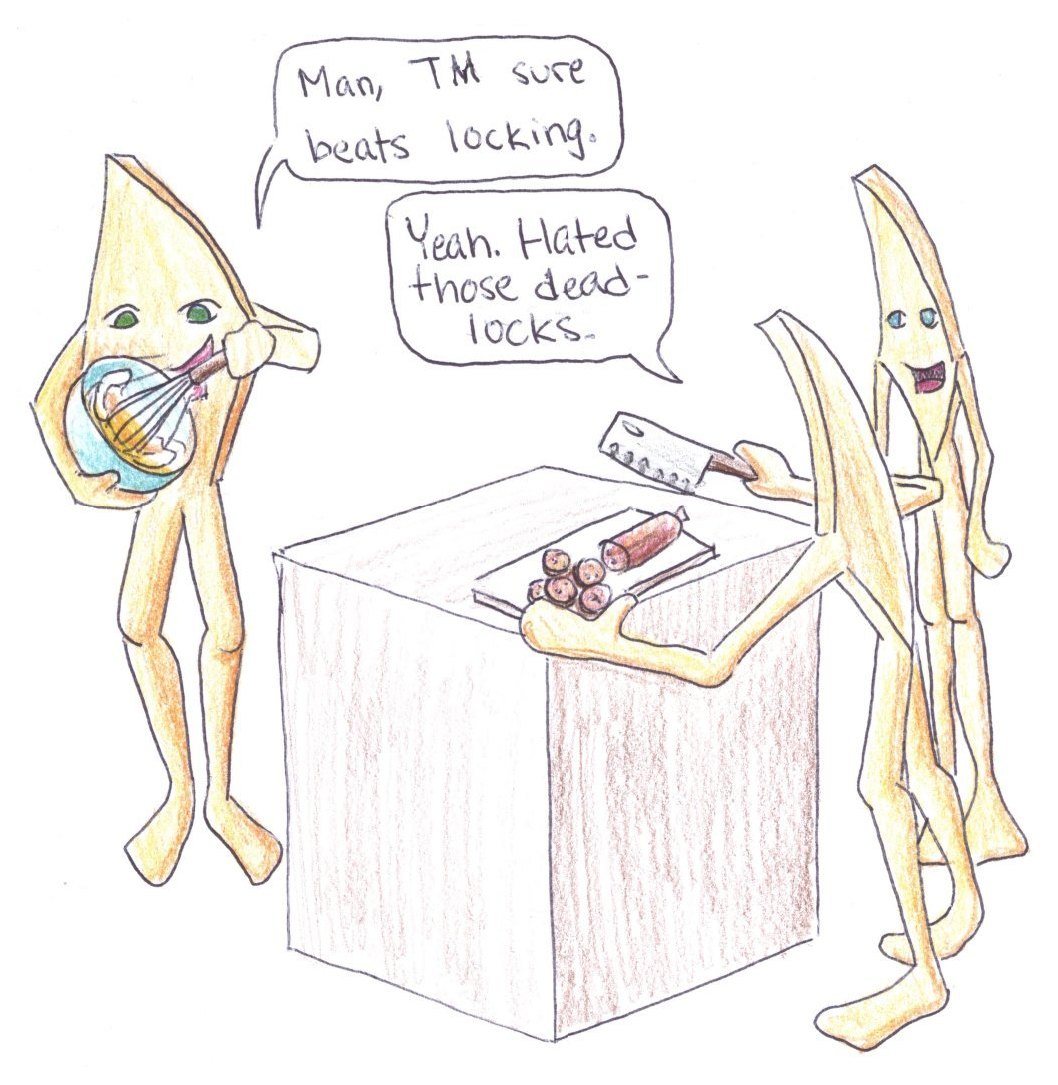
\includegraphics{cartoons/TM-the-vision}}
\caption{The STM Vision}
\ContributedBy{Figure}{fig:future:The STM Vision}{Melissa Broussard}
\end{figure}

\begin{figure}[tb]
\centering
\resizebox{3in}{!}{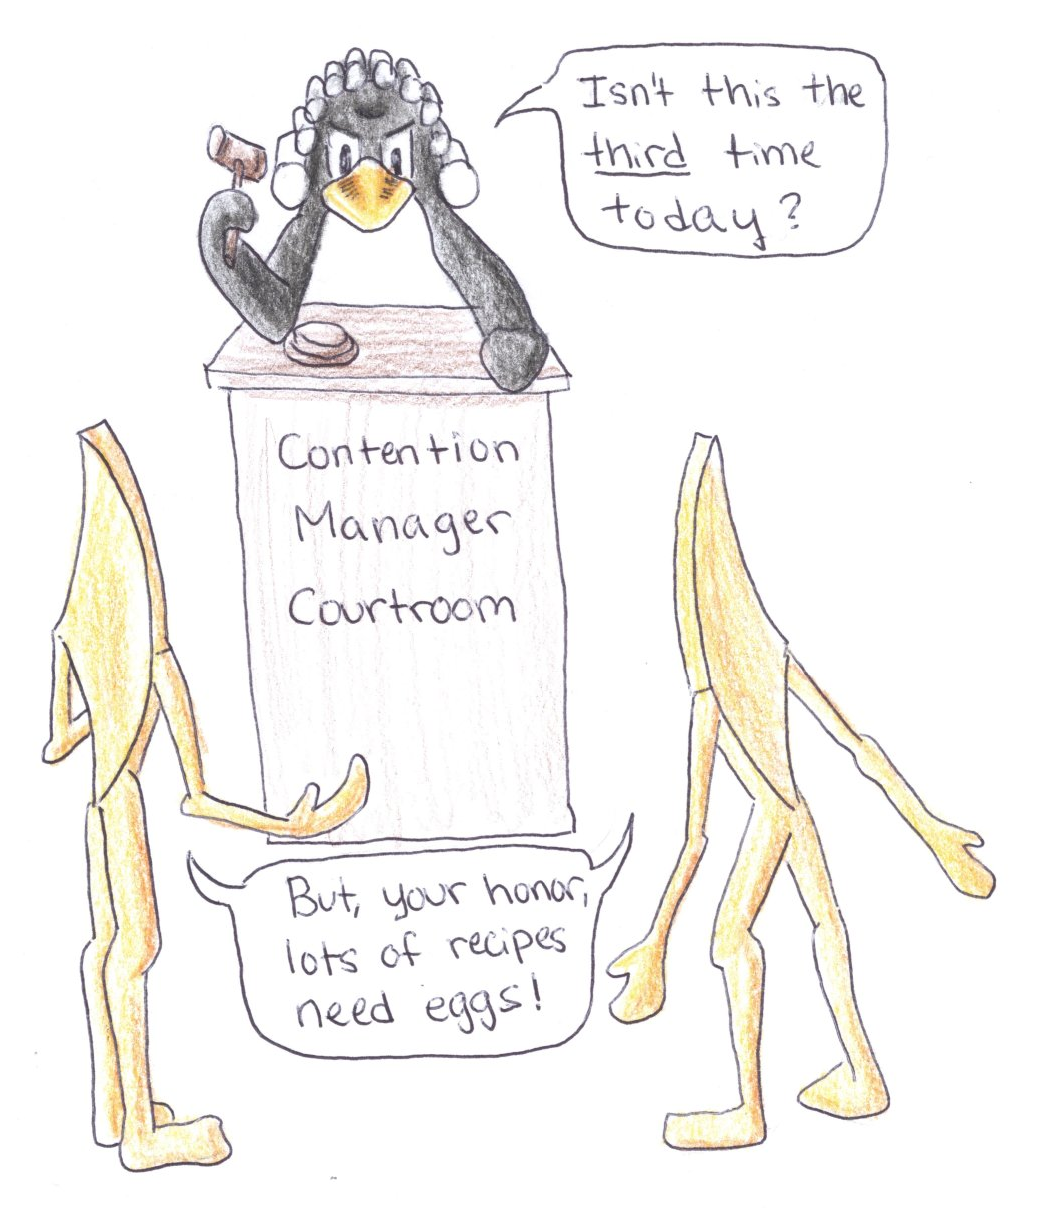
\includegraphics{cartoons/TM-the-reality-conflict}}
\caption{The STM Reality: Conflicts}
\ContributedBy{Figure}{fig:future:The STM Reality: Conflicts}{Melissa Broussard}
\end{figure}

\begin{figure}[tb]
\centering
\resizebox{3in}{!}{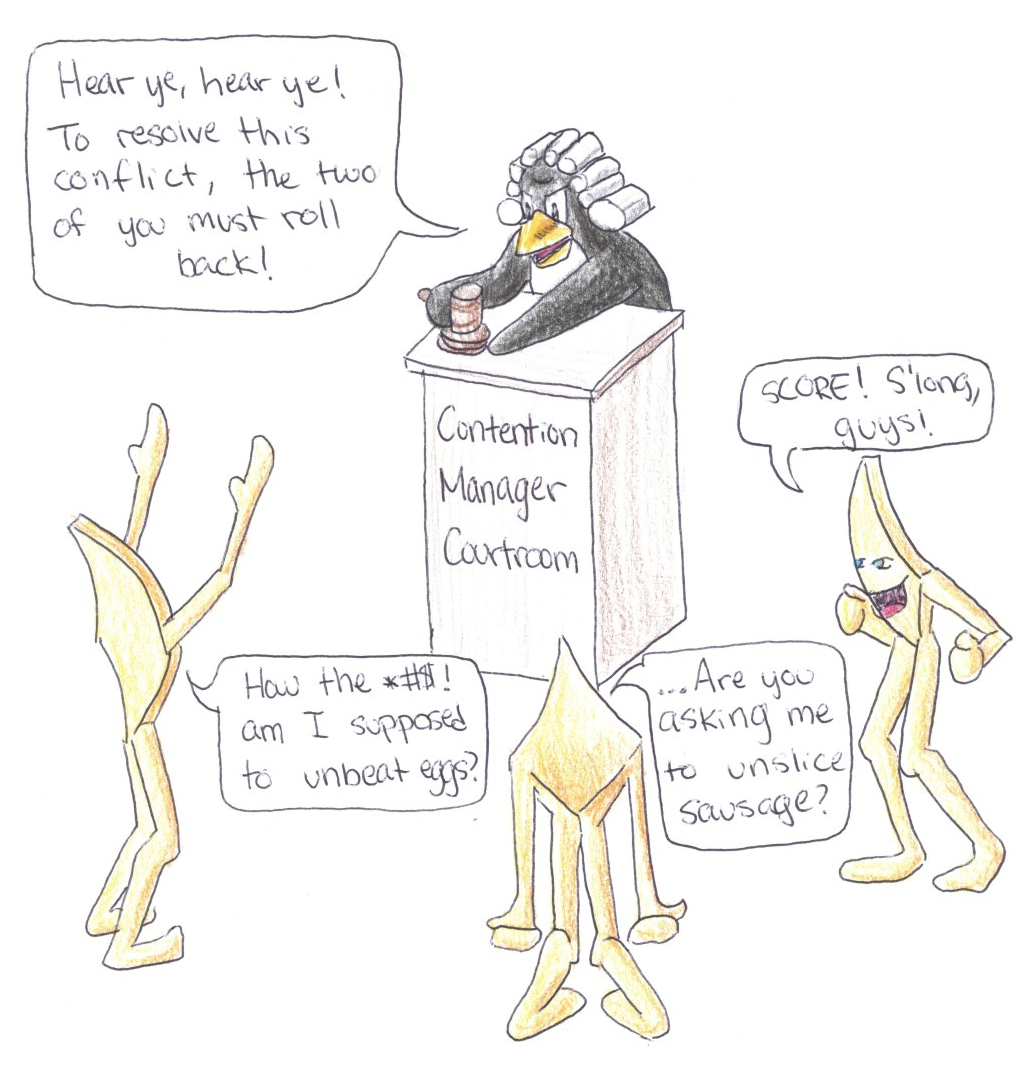
\includegraphics{cartoons/TM-the-reality-nonidempotent}}
\caption{The STM Reality: Irrevocable Operations}
\ContributedBy{Figure}{fig:future:The STM Reality: Irrevocable Operations}{Melissa Broussard}
\end{figure}

\begin{figure}[tb]
\centering
\resizebox{3in}{!}{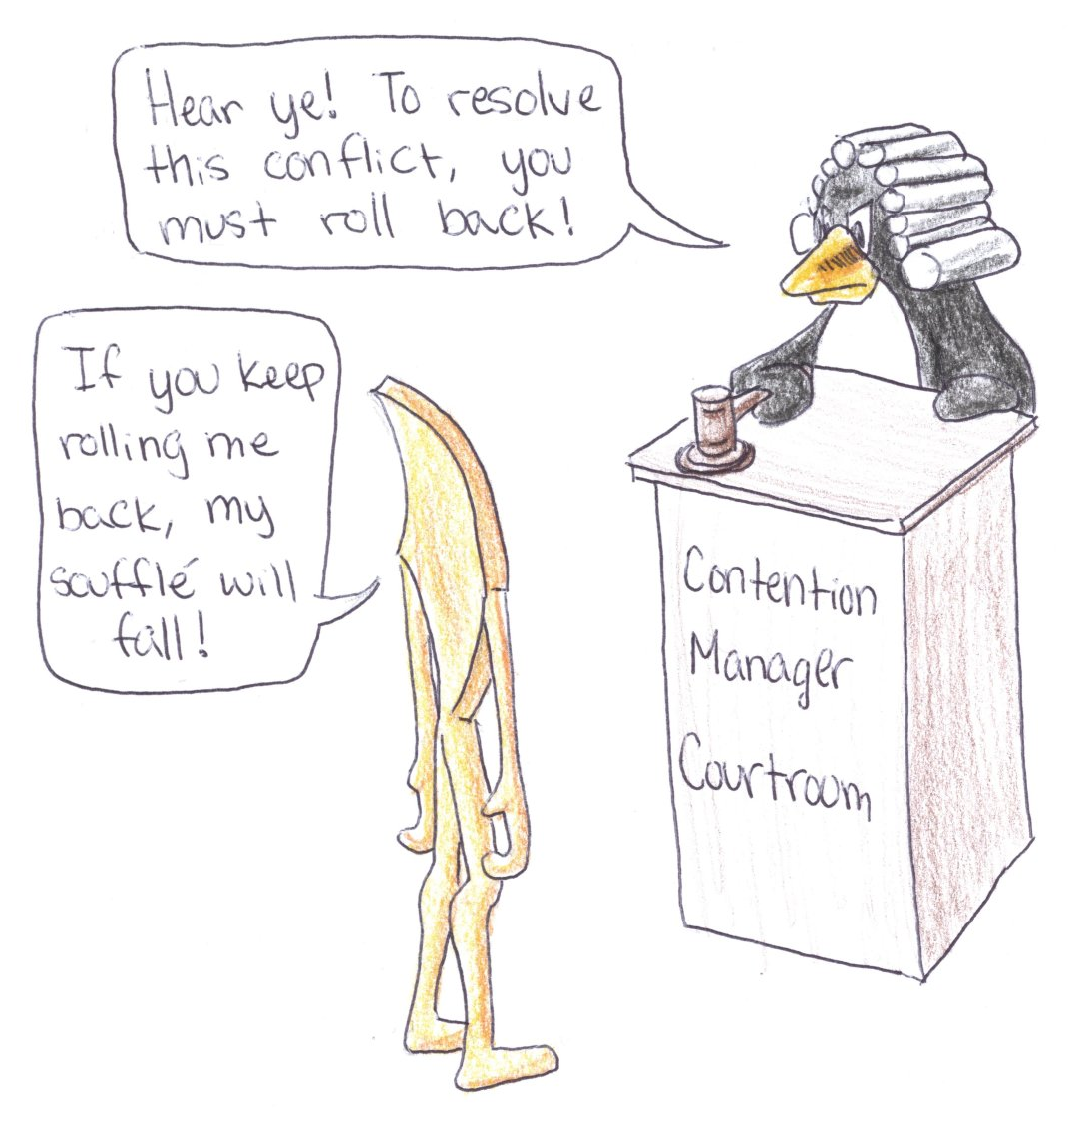
\includegraphics{cartoons/TM-the-reality-realtime}}
\caption{The STM Reality: Realtime Response}
\ContributedBy{Figure}{fig:future:The STM Reality: Realtime Response}{Melissa Broussard}
\end{figure}

But for the moment, the current state of STM
can best be summarized with a series of cartoons.
First,
Figure~\ref{fig:future:The STM Vision}
shows the STM vision.
As always, the reality is a bit more nuanced, as fancifully depicted by
Figures~\ref{fig:future:The STM Reality: Conflicts},
\ref{fig:future:The STM Reality: Irrevocable Operations},
and~\ref{fig:future:The STM Reality: Realtime Response}.

Recent advances in commercially available hardware have opened the door
for variants of HTM, which are addressed in the following section.

% @@@ Don Porter's user-level TM work for Linux.

% future/htm.tex

\section{Hardware Transactional Memory}
\label{sec:future:Hardware Transactional Memory}

As of early 2012, hardware transactional memory (HTM) is starting to emerge
into commercially available commodity computer systems.
This section makes a first attempt to find its place in the parallel
programmer's toolbox.

From a conceptual viewpoint, HTM uses processor caches and speculative
execution to make a designated group of statements (a ``transaction'')
take effect atomically
from the viewpoint of any other transactions running on other processors.
This transaction is initiated by a
begin-transaction machine instruction and completed by a commit-transaction
machine instruction.
There is typically also an abort-transaction machine instruction, which
squashes the speculation (as if the begin-transaction instruction and
all following instructions had not executed) and commences execution
at a failure handler.
The location of the failure handler is typically specified by the
begin-transaction instruction, either as an explicit failure-handler
address or via a condition code set by the instruction itself.
Each transaction executes atomically with respect to all other transactions.

HTM has a number of important benefits, including automatic
dynamic partitioning of data structures, reducing synchronization-primitive
cache misses, and supporting a fair number of practical applications.

However, it always pays to read the fine print, and HTM is no exception.
A major point of this section is determining under what conditions HTM's
benefits outweigh the complications hidden in its fine print.
To this end, Section~\ref{sec:future:HTM Benefits WRT to Locking}
describes HTM's benefits and
Section~\ref{sec:future:HTM Weaknesses WRT Locking} describes its weaknesses.
This is the same approach used in earlier
papers~\cite{McKenney2007PLOSTM,PaulEMcKenney2010OSRGrassGreener},
but focused on HTM rather than TM as a whole.\footnote{
	And I gratefully acknowledge many stimulating
	discussions with the other authors, Maged Michael, Josh Triplett,
	and Jonathan Walpole, as well as with Andi Kleen.}

Section~\ref{sec:future:HTM Weaknesses WRT to Locking When Augmented} then describes
HTM's weaknesses with respect to the combination of synchronization
primitives used in the Linux kernel (and in some user-space applications).
Section~\ref{sec:future:Where Does HTM Best Fit In?} looks at where HTM
might best fit into the parallel programmer's toolbox, and
Section~\ref{sec:future:Potential Game Changers} lists some events that might
greatly increase HTM's scope and appeal.
Finally, Section~\ref{sec:future:Conclusions}
presents concluding remarks.

\subsection{HTM Benefits WRT to Locking}
\label{sec:future:HTM Benefits WRT to Locking}

The primary benefits of HTM are
(1)~its avoidance of the cache misses that are often incurred by
other synchronization primitives,
(2)~its ability to dynamically partition
data structures,
and (3)~the fact that it has
a fair number of practical applications.
I break from TM tradition by not listing ease of use separately
for two reasons.
First, ease of use should stem from HTM's primary benefits,
which this section focuses on.
Second, there has been considerable controversy surrounding attempts to
test for raw programming
talent~\cite{RichardBornat2006SheepGoats,SaeedDehnadi2009SheepGoats}
and even around the use of small programming exercises in job
interviews~\cite{RegBraithwaite2007FizzBuzz}.
This indicates that we really do not have a grasp on what makes
programming easy or hard.
Therefore, this section focuses on the three benefits listed above,
each in one of the following sections.

\subsubsection{Avoiding Synchronization Cache Misses}
\label{sec:future:Avoiding Synchronization Cache Misses}

Most synchronization mechanisms are based on data structures that are
operated on by atomic instructions.
Because these atomic instructions normally operate by first causing
the relevant cache line to be owned by the CPU that they are running on,
a subsequent execution
of the same instance of that synchronization primitive on some other
CPU will result in a cache miss.
These communications cache misses severely degrade both the performance and
scalability of conventional synchronization
mechanisms~\cite[Section 4.2.3]{Anderson97}.

In contrast, HTM synchronizes by using the CPU's cache, avoiding the need
for a synchronization data structure and resultant cache misses.
HTM's advantage is greatest in cases where a lock data structure is
placed in a separate cache line, in which case, converting a given
critical section to an HTM transaction can reduce that critical section's
overhead by a full cache miss.
These savings can be quite significant for the common case of short
critical sections, at least for those situations where the elided lock
does not share a cache line with an oft-written variable protected by
that lock.

\QuickQuiz{}
	Why would it matter that oft-written variables shared the cache
	line with the lock variable?
\QuickQuizAnswer{
	If the lock is in the same cacheline as some of the variables
	that it is protecting, then writes to those variables by one CPU
	will invalidate that cache line for all the other CPUs.
	These invalidations will
	generate large numbers of conflicts and retries, perhaps even
	degrading performance and scalability compared to locking.
} \QuickQuizEnd

\subsubsection{Dynamic Partitioning of Data Structures}
\label{sec:future:Dynamic Partitioning of Data Structures}

A major obstacle to the use of some conventional synchronization mechanisms
is the need to statically partition data structures.
There are a number of data structures that are trivially
partitionable, with the most prominent example being hash tables,
where each hash chain constitutes a partition.
Allocating a lock for each hash chain then trivially parallelizes
the hash table for operations confined to a given chain.\footnote{
	And it is also easy to extend this scheme to operations accessing
	multiple hash chains by having such operations acquire the
	locks for all relevant chains in hash order.}
Partitioning is similarly trivial for arrays, radix trees, and a few
other data structures.

However, partitioning for many types of trees and graphs is quite
difficult, and the results are often quite complex~\cite{Ellis80}.
Although it is possible to use two-phased locking and hashed arrays
of locks to partition general data structures, other techniques
have proven preferable~\cite{DavidSMiller2006HashedLocking},
as will be discussed in
Section~\ref{sec:future:HTM Weaknesses WRT to Locking When Augmented}.
Given its avoidance of synchronization cache misses,
HTM is therefore a very real possibility for large non-partitionable
data structures, at least assuming relatively small updates.

\QuickQuiz{}
	Why are relatively small updates important to HTM performance
	and scalability?
\QuickQuizAnswer{
	The larger the updates, the greater the probability of conflict,
	and thus the greater probability of retries, which degrade
	performance.
} \QuickQuizEnd

\subsubsection{Practical Value}
\label{sec:future:Practical Value}

Some evidence of HTM's practical value has been demonstrated in a number
of hardware platforms, including
Sun Rock~\cite{DaveDice2009ASPLOSRockHTM} and
Azul Vega~\cite{CliffClick2009AzulHTM}.
It is reasonable to assume that practical benefits will flow from the
more recent IBM Blue Gene/Q, Intel Haswell TSX, and AMD ASF systems.

Expected practical benefits include:

\begin{enumerate}
\item	Lock elision for in-memory data access and
	update~\cite{Martinez01a,Rajwar02a}.
\item	Concurrent access and small random updates to large non-partitionable
	data structures.
\end{enumerate}

However, HTM also has some very real shortcomings, which will be discussed
in the next section.

\subsection{HTM Weaknesses WRT Locking}
\label{sec:future:HTM Weaknesses WRT Locking}

The concept of HTM is quite simple: A group of accesses and updates to
memory occurs atomically.
However, as is the case with many simple ideas, complications arise
when you apply it to real systems in the real world.
These complications are as follows:

\begin{enumerate}
\item	Transaction-size limitations.
\item	Conflict handling.
\item	Aborts and rollbacks.
\item	Lack of forward-progress guarantees.
\item	Irrevocable operations.
\item	Semantic differences.
\end{enumerate}

Each of these complications is covered in the following sections,
followed by a summary.

\subsubsection{Transaction-Size Limitations}
\label{sec:future:Transaction-Size Limitations}

The transaction-size limitations of current HTM implementations
stem from the use of the processor caches to hold the data
affected by the transaction.
Although this allows a given CPU to make the transaction appear atomic to
other CPUs by executing the transaction within the confines of its cache,
it also means that any transaction that does not fit must be aborted.
Furthermore, events that change execution context, such as interrupts,
system calls, exceptions, traps, and context switches either must
abort any ongoing transaction on the CPU in question or must further
restrict transaction size due to the cache footprint of the other
execution context.

Of course, modern CPUs tend to have large caches, and the data required
for many transactions would fit easily in a one-megabyte cache.
Unfortunately, with caches, sheer size is not all that matters.
The problem is that most caches
can be thought of hash tables implemented in hardware.
However, hardware caches do not chain their buckets (which are normally
called \emph{sets}), but rather
provide a fixed number of cachelines per set.
The number of elements provided for each set in a given cache
is termed that cache's \emph{associativity}.

Although cache associativity varies, the eight-way associativity of
the level-0 cache on the laptop I am typing this on is not unusual.
What this means is that if a given transaction needed to touch
nine cache lines, and if all nine cache lines mapped to the same
set, then that transaction cannot possibly complete, never mind how
many megabytes of additional space might be available in that cache.
Yes, given randomly selected data elements in a given data structure,
the probability of that transaction being able to commit is quite
high, but there can be no guarantee.

There has been some research work to alleviate this limitation.
Fully associative \emph{victim caches} would alleviate the associativity
constraints, but there are currently stringent performance and
energy-efficiency constraints on the sizes of victim caches.
That said, HTM victim caches for unmodified cache lines can be quite
small, as they need to retain only the address:
The data itself can be written to memory or shadowed by other caches,
while the address itself is sufficient to detect a conflicting
write~\cite{RaviRajwar2012TSX}.

\emph{Unbounded transactional memory} (UTM)
schemes~\cite{CScottAnanian2006,KevinEMoore2006}
use DRAM as an extremely large victim cache, but integrating such schemes
into a production-quality cache-coherence mechanism is still an unsolved
problem.
In addition, use of DRAM as a victim cache may have unfortunate
performance and energy-efficiency consequences, particularly
if the victim cache is to be fully associative.
Finally, the ``unbounded'' aspect of UTM assumes that all of DRAM
could be used as a victim cache, while in reality
the large but still fixed amount of DRAM assigned to a given CPU
would limit the size of that CPU's transactions.
Other schemes use a combination of hardware and software transactional
memory~\cite{SanjeevKumar2006} and one could imagine using STM as a
fallback mechanism for HTM.

However, to the best of my knowledge, currently available systems do
not implement any of these research ideas, and perhaps for good reason.

\subsubsection{Conflict Handling}
\label{sec:future:Conflict Handling}

The first complication is the possibility of \emph{conflicts}.
For example, suppose that transactions~A and~B are defined as follows:

\vspace{5pt}
\begin{minipage}[t]{\columnwidth}
\begin{verbatim}
Transaction A       Transaction B

x = 1;              y = 2;
y = 3;              x = 4;
\end{verbatim}
\end{minipage}
\vspace{5pt}

Suppose that each transaction executes concurrently on its own processor.
If transaction~A stores to \co{x} at the same time that transaction~B
stores to \co{y}, neither transaction can progress.
To see this, suppose that transaction~A executes its store to \co{y}.
Then transaction~A will be interleaved within transaction~B, in violation
of the requirement that transactions execute atomically with respect to
each other.
Allowing transaction~B to execute its store to \co{x} similarly violates
the atomic-execution requirement.
This situation is termed a \emph{conflict}, which happens whenever two
concurrent transactions access the same variable where at least one of
the accesses is a store.
The system is therefore obligated to abort one or both of the transactions
in order to allow execution to progress.
The choice of exactly which transaction to abort is an interesting topic
that will very likely retain the ability to generate Ph.D. dissertations for
some time to come, see for
example~\cite{EgeAkpinar2011HTM2TLE}.\footnote{
	Liu's and Spear's paper entitled ``Toxic
	Transactions''~\cite{YujieLiu2011ToxicTransactions} is
	particularly instructive in this regard.}
For the purposes of this section, we can assume that the system makes
a random choice.

Another complication is conflict detection, which is comparatively
straightforward, at least in the simplest case.
When a processor is executing a transaction, it marks every cache line
touched by that transaction.
If the processor's cache receives a request involving a cache line that
has been marked as touched by the current transaction, a potential
conflict has occurred.
More sophisticated systems might try to order the current processors'
transaction to precede that of the processor sending the request,
and optimization of this process will likely also retain the ability
to generate Ph.D. dissertations for quite some time.
However this section assumes a very simple conflict-detection strategy.

However, for HTM to work effectively, the probability of conflict must
be suitably low, which in turn requires that the data structures
be organized so as to maintain a sufficiently low probability of conflict.
For example, a red-black tree with simple insertion, deletion, and search
operations fits this description, but a red-black
tree that maintains an accurate count of the number of elements in
the tree does not.\footnote{
	The need to update the count would result in additions to and
	deletions from the tree conflicting with each other, resulting
	in strong non-commutativity~\cite{HagitAttiya2011LawsOfOrder,Attiya:2011:LOE:1925844.1926442,PaulEMcKenney2011SNC}.}
For another example, a red-black tree that enumerates all elements in
the tree in a single transaction will have high conflict probabilities,
degrading performance and scalability.
As a result, many serial programs will require some restructuring before
HTM can work effectively.
In some cases, practitioners will prefer to take the extra steps
(in the red-black-tree case, perhaps switching to a partitionable
data structure such as a radix tree or a hash table), and just
use locking, particularly during the time before HTM is readily available
on all relevant
architectures~\cite{CliffClick2009AzulHTM}.

\QuickQuiz{}
	How could a red-black tree possibly efficiently enumerate all
	elements of the tree regardless of choice of synchronization
	mechanism???
\QuickQuizAnswer{
	In many cases, the enumeration need not be exact.
	In these cases, hazard pointers or RCU may be used to protect
	readers with low probability of conflict with any given insertion
	or deletion.
} \QuickQuizEnd

Furthermore, the fact that conflicts can occur brings failure handling
into the picture, as discussed in the next section.

\subsubsection{Aborts and Rollbacks}
\label{sec:future:Aborts and Rollbacks}

Because any transaction might be aborted at any time, it is important
that transactions contain no statements that cannot be rolled back.
This means that transactions cannot do I/O, system calls, or debugging
breakpoints (no single stepping in the debugger for HTM transactions!!!).
Instead, transactions must confine themselves to accessing normal
cached memory.
Furthermore, on some systems, interrupts, exceptions, traps,
TLB misses, and other events will also abort transactions.
Given the number of bugs that have resulted from improper handling
of error conditions, it is fair to ask what impact aborts and rollbacks
have on ease of use.

\QuickQuiz{}
	But why can't a debugger emulate single stepping by setting
	breakpoints at successive lines of the transaction, relying
	on the retry to retrace the steps of the earlier instances
	of the transaction?
\QuickQuizAnswer{
	This scheme might work with reasonably high probability, but it
	can fail in ways that would be quite surprising to most users.
	To see this, consider the following transaction:

	\vspace{5pt}
	\begin{minipage}[t]{\columnwidth}
	\small
\begin{verbatim}
  1 begin_trans();
  2 if (a) {
  3   do_one_thing();
  4   do_another_thing();
  5 } else {
  6   do_a_third_thing();
  7   do_a_fourth_thing();
  8 }
  9 end_trans();
\end{verbatim}
	\end{minipage}
	\vspace{5pt}

	Suppose that the user sets a breakpoint at line 3, which triggers,
	aborting the transaction and entering the debugger.
	Suppose that between the time that the breakpoint triggers
	and the debugger gets around to stopping all the threads, some
	other thread sets the value of \co{a} to zero.
	When the poor user attempts to single-step the program, surprise!
	The program is now in the else-clause instead of the then-clause.

	This is \emph{not} what I call an easy-to-use debugger.
} \QuickQuizEnd

Of course, aborts and rollbacks raise the question of whether HTM can
be useful for hard real-time systems.
Do the performance benefits of HTM outweigh the costs of the aborts
and rollbacks, and if so under what conditions?
Can transactions use priority boosting?
Or should transactions for high-priority threads instead preferentially
abort those of low-priority threads?
If so, how is the hardware efficiently informed of priorities?
The literature on real-time use of HTM is quite sparse, perhaps because
researchers are finding more than enough problems in getting
transactions to work well in non-real-time environments.

Because current HTM implementations might deterministically abort a
given transaction, software must provide fallback code.
This fallback code must use some other form of synchronization, for
example, locking.
If the fallback is used frequently, then all the limitations of locking,
including the possibility of deadlock, reappear.
One can of course hope that the fallback isn't used often, which might
allow simpler and less deadlock-prone locking designs to be used.
But this raises the question of how the system transitions from using
the lock-based fallbacks back to transactions.\footnote{
	The possibility of an application getting stuck in fallback
	mode has been termed the ``lemming effect'', a term that
	Dave Dice has been credited with coining.}
One approach is to use a test-and-test-and-set discipline~\cite{Martinez02a},
so that everyone holds off until the lock is released, allowing the
system to start from a clean slate in transactional mode at that point.
However, this could result in quite a bit of spinning, which might not
be wise if the lock holder has blocked or been preempted.
Another approach is to allow transactions to proceed in parallel with
a thread holding a lock~\cite{Martinez02a}, but this raises difficulties
in maintaining atomicity, especially if the reason that the thread is
holding the lock is because the corresponding transaction would not fit
into cache.

Finally, dealing with the possibility of aborts and rollbacks seems to
put an additional burden on the developer, who must correctly handle
all combinations of possible error conditions.

It is clear that users of HTM must put considerable validation effort
into testing both the fallback code paths and transition from fallback
code back to transactional code.

\subsubsection{Lack of Forward-Progress Guarantees}
\label{sec:future:Lack of Forward-Progress Guarantees}

Even though transaction size, conflicts, and aborts/rollbacks can all
cause transactions to abort, one might hope that sufficiently small and
short-duration transactions could be guaranteed to eventually succeed.
This would permit a transaction to be unconditionally retried, in the
same way that compare-and-swap (CAS) and load-linked/store-conditional
(LL/SC) operations are unconditionally retried in code that uses these
instructions to implement atomic operations.

Unfortunately, most currently available HTM implementation refuse to
make any
sort of forward-progress guarantee, which means that HTM cannot be
used to avoid deadlock on those systems.\footnote{
	HTM might well be used to reduce the probability of deadlock,
	but as long as there is some possibility of the fallback
	code being executed, there is some possibility of deadlock.}
Hopefully future implementations of HTM will provide some sort of
forward-progress guarantees.
Until that time, HTM must be used with extreme caution in real-time
applications.\footnote{
	As of mid-2012, there has been surprisingly little work on
	transactional memory's real-time characteristics.}

The one exception to this gloomy picture as of 2013 is upcoming versions
of the IBM mainframe, which provides a separate instruction that may be
used to start a special
\emph{constrained transaction}~\cite{ChristianJacobi2012MainframeTM}.
As you might guess from the name, such transactions must live within
the following constraints:

\begin{enumerate}
\item	Each transaction's data footprint must be contained within
	four 32-byte blocks of memory.
\item	Each transaction is permitted to execute at most 32 assembler
	instructions.
\item	Transactions are not permitted to have backwards branches
	(e.g., no loops).
\item	Each transaction's code is limited to 256 bytes of memory.
\item	If a portion of a given transaction's data footprint resides
	within a given 4K page, then that 4K page is prohibited from
	containing any of that transaction's instructions.
\end{enumerate}

These constraints are severe, but they nevertheless permit a wide variety
of data-structure updates to be implemented, including stacks, queues,
hash tables, and so on.
These operations are guaranteed to eventually complete, and are free of
deadlock and livelock conditions.

It will be interesting to see how hardware support of forward-progress
guarantees evolves over time.

\subsubsection{Irrevocable Operations}
\label{sec:future:Irrevocable Operations}

Another consequence of aborts and rollbacks is that HTM transactions
cannot accommodate irrevocable operations.
Current HTM implementations typically enforce this limitation by
requiring that all of the accesses in the transaction be to cacheable
memory (thus prohibiting MMIO accesses) and aborting transactions on
interrupts, traps, and exceptions (thus prohibiting system calls).

Note that buffered I/O can be accommodated by HTM transactions as
long as the buffer fill/flush operations occur extra-transactionally.
The reason that this works is that adding data to and removing data
from the buffer is revocable: Only the actual buffer fill/flush
operations are irrevocable.
Of course, this buffered-I/O approach has the effect of including the I/O
in the transaction's footprint, increasing the size of the transaction
and thus increasing the probability of failure.

\subsubsection{Semantic Differences}
\label{sec:future:Semantic Differences}

Although HTM can in many cases be used as a drop-in replacement for locking
(hence the name transactional lock
elision~\cite{DaveDice2008TransactLockElision}),
there are subtle differences in semantics.
A particularly nasty example involving coordinated lock-based critical
sections that results in deadlock or livelock when executed transactionally
was given by Blundell~\cite{Blundell2006TMdeadlock}, but a much simpler
example is the empty critical section.

In a lock-based program, an empty critical section will guarantee
that all processes that had previously been holding that lock have
now released it.
This idiom was used by the 2.4 Linux kernel's networking stack to
coordinate changes in configuration.
But if this empty critical section is translated to a transaction,
the result is a no-op.
The guarantee that all prior critical sections have terminated is
lost.
In other words, transactional lock elision preserves the data-protection
semantics of locking, but loses locking's time-based messaging semantics.

\QuickQuiz{}
	But why would \emph{anyone} need an empty lock-based critical
	section???
\QuickQuizAnswer{
	See the answer to \QuickQuizARef{\QlockingQemptycriticalsection} in
	Section~\ref{sec:locking:Exclusive Locks}.

	However, it is claimed that given a strongly atomic HTM
	implementation without forward-progress guarantees, any
	memory-based locking design based on empty critical sections
	will operate correctly in the presence of transactional
	lock elision.
	Although I have not seen a proof of this statement, there
	is a straightforward rationale for this claim.
	The main idea is that in a strongly atomic HTM implementation,
	the results of a given transaction are not visible until
	after the transaction completes successfully.
	Therefore, if you can see that a transaction has started,
	it is guaranteed to have already completed, which means
	that a subsequent empty lock-based critical section will
	successfully ``wait'' on it---after all, there is no waiting
	required.

	This line of reasoning does not apply to weakly atomic
	systems (including many STM implementation), and it also
	does not apply to lock-based programs that use means other
	than memory to communicate.
	One such means is the passage of time (for example, in
	hard real-time systems) or flow of priority (for example,
	in soft real-time systems).

	Locking designs that rely on priority boosting are of particular
	interest.
} \QuickQuizEnd

\QuickQuiz{}
	Can't transactional lock elision trivially handle locking's
	time-based messaging semantics
	by simply choosing not to elide empty lock-based critical sections?
\QuickQuizAnswer{
	It could do so, but this would be both unnecessary and
	insufficient.

	It would be unnecessary in cases where the empty critical section
	was due to conditional compilation.
	Here, it might well be that the only purpose of the lock was to
	protect data, so eliding it completely would be the right thing
	to do.
	In fact, leaving the empty lock-based critical section would
	degrade performance and scalability.

	On the other hand, it is possible for a non-empty lock-based
	critical section to be relying on both the data-protection
	and time-based and messaging semantics of locking.
	Using transactional lock elision in such a case would be
	incorrect, and would result in bugs.
} \QuickQuizEnd

\QuickQuiz{}
	Given modern hardware~\cite{PeterOkech2009InherentRandomness},
	how can anyone possibly expect parallel software relying
	on timing to work?
\QuickQuizAnswer{
	The short answer is that on commonplace commodity hardware,
	synchronization designs based on any sort of fine-grained
	timing are foolhardy and cannot be expected to operate correctly
	under all conditions.

	That said, there are systems designed for hard real-time use
	that are much more deterministic.
	In the (very unlikely) event that you are using such a system,
	here is a toy example showing how time-based synchronization can
	work.
	Again, do \emph{not} try this on commodity microprocessors,
	as they have highly nondeterministic performance characteristics.

	This example uses multiple worker threads along with a control
	thread.
	Each worker thread corresponds to an outbound data feed, and
	records the current time (for example, from the
	\co{clock_gettime()} system call) in a per-thread
	\co{my_timestamp} variable after executing each unit
	of work.
	The real-time nature of this example results in the following
	set of constraints:

	\begin{enumerate}
	\item	It is a fatal error for a given worker thread to fail
		to update its timestamp for a time period of more than
		\co{MAX_LOOP_TIME}.
	\item	Locks are used sparingly to access and update global
		state.
	item	Locks are granted in strict FIFO order within
		a given thread priority.
	\end{enumerate}

	When worker threads complete their feed, they must disentangle
	themselves from the rest of the application and place a status
	value in a per-thread \co{my_status} variable that is initialized
	to $-1$.
	Threads do not exit; they instead are placed on a thread pool
	to accommodate later processing requirements.
	The control thread assigns (and re-assigns) worker threads as
	needed, and also maintains a histogram of thread statuses.
	The control thread runs at a real-time priority no higher than
	that of the worker threads.

	Worker threads' code is as follows:

	\vspace{5pt}
	\begin{minipage}[t]{\columnwidth}
	\scriptsize
\begin{verbatim}
  1   int my_status = -1;  /* Thread local. */
  2 
  3   while (continue_working()) {
  4     enqueue_any_new_work();
  5     wp = dequeue_work();
  6     do_work(wp);
  7     my_timestamp = clock_gettime(...);
  8   }
  9 
 10   acquire_lock(&departing_thread_lock);
 11 
 12   /*
 13    * Disentangle from application, might
 14    * acquire other locks, can take much longer
 15    * than MAX_LOOP_TIME, especially if many
 16    * threads exit concurrently.
 17    */
 18   my_status = get_return_status();
 19   release_lock(&departing_thread_lock);
 20 
 21   /* thread awaits repurposing. */
\end{verbatim}
	\end{minipage}
	\vspace{5pt}

	The control thread's code is as follows:

	\vspace{5pt}
	\begin{minipage}[t]{\columnwidth}
	\scriptsize
\begin{verbatim}
  1   for (;;) {
  2     for_each_thread(t) {
  3       ct = clock_gettime(...);
  4       d = ct - per_thread(my_timestamp, t);
  5       if (d >= MAX_LOOP_TIME) {
  6         /* thread departing. */
  7         acquire_lock(&departing_thread_lock);
  8         release_lock(&departing_thread_lock);
  9         i = per_thread(my_status, t);
 10         status_hist[i]++; /* Bug if TLE! */
 11       }
 12     }
 13     /* Repurpose threads as needed. */
 14   }
\end{verbatim}
	\end{minipage}
	\vspace{5pt}

	Line~5 uses the passage of time to deduce that the thread
	has exited, executing lines~6-10 if so.
	The empty lock-based critical section on lines~7 and~8
	guarantees that any thread in the process of exiting
	completes (remember that locks are granted in FIFO order!).

	Once again, do not try this sort of thing on commodity
	microprocessors.
	After all, it is difficult enough to get right on systems
	specifically designed for hard real-time use!
} \QuickQuizEnd

One important semantic difference between locking and transactions
is the priority boosting that is used to avoid priority inversion
in lock-based real-time programs.
One way in which priority inversion can occur is when a
low-priority thread holding a lock
is preempted by a medium-priority CPU-bound thread.
If there is at least one such medium-priority thread per CPU, the
low-priority thread will never get a chance to run.
If a high-priority thread now attempts to acquire the lock,
it will block.
It cannot acquire the lock until the low-priority thread releases it,
the low-priority thread cannot release the lock until it gets a chance
to run, and it cannot get a chance to run until one of the medium-priority
threads gives up its CPU.
Therefore, the medium-priority threads are in effect blocking the
high-priority process, which is the rationale for the name ``priority
inversion.''

\begin{figure}[tbp]
{ \scriptsize
\begin{verbbox}
  1 void boostee(void)
  2 {
  3   int i = 0;
  4 
  5   acquire_lock(&boost_lock[i]);
  6   for (;;) {
  7     acquire_lock(&boost_lock[!i]);
  8     release_lock(&boost_lock[i]);
  9     i = i ^ 1;
 10     do_something();
 11   }
 12 }
 13 
 14 void booster(void)
 15 {
 16   int i = 0;
 17 
 18   for (;;) {
 19     usleep(1000); /* sleep 1 ms. */
 20     acquire_lock(&boost_lock[i]);
 21     release_lock(&boost_lock[i]);
 22     i = i ^ 1;
 23   }
 24 }
\end{verbbox}
}
\centering
\theverbbox
\caption{Exploiting Priority Boosting}
\label{fig:future:Exploiting Priority Boosting}
\end{figure}

One way to avoid priority inversion is \emph{priority inheritance},
in which a high-priority thread blocked on a lock temporarily donates
its priority to the lock's holder, which is also called \emph{priority
boosting}.
However, priority boosting can be used for things other than avoiding
priority inversion, as shown in
Figure~\ref{fig:future:Exploiting Priority Boosting}.
Lines~1-12 of this figure show a low-priority process that must
nevertheless run every millisecond or so, while lines~14-24 of
this same figure show a high-priority process that uses priority
boosting to ensure that \co{boostee()} runs periodically as needed.

The \co{boostee()} function arranges this by always holding one of
the two \co{boost_lock[]} locks, so that lines~20-21 of
\co{booster()} can boost priority as needed.

\QuickQuiz{}
	But the \co{boostee()} function in
	Figure~\ref{fig:future:Exploiting Priority Boosting}
	alternatively acquires its locks in reverse order!
	Won't this result in deadlock?
\QuickQuizAnswer{
	No deadlock will result.
	To arrive at deadlock, two different threads must each
	acquire the two locks in oppposite orders, which does not
	happen in this example.
	However, deadlock detectors such as
	lockdep~\cite{JonathanCorbet2006lockdep}
	will flag this as a false positive.
} \QuickQuizEnd

This arrangement requires that \co{boostee()} acquire its first
lock on line~5 before the system becomes busy, but this is easily
arranged, even on modern hardware.

Unfortunately, this arrangement can break down in presence of transactional
lock elision.
The \co{boostee()} function's overlapping critical sections become
one infinite transaction, which will sooner or later abort,
for example, on the first time that the thread running
the \co{boostee()} function is preempted.
At this point, \co{boostee()} will fall back to locking, but given
its low priority and that the quiet initialization period is now
complete (which after all is why \co{boostee()} was preempted),
this thread might never again get a chance to run.

And if the \co{boostee()} thread is not holding the lock, then
the \co{booster()} thread's empty critical section on lines~20 and~21 of
Figure~\ref{fig:future:Exploiting Priority Boosting}
will become an empty transaction that has no effect, so that
\co{boostee()} never runs.
This example illustrates some of the subtle consequences of
transactional memory's rollback-and-retry semantics.

Given that experience will likely uncover additional subtle semantic
differences, application of HTM-based lock elision to large programs
should be undertaken with caution.
That said, where it does apply, HTM-based lock elision can eliminate
the cache misses associated with the lock variable, which has resulted
in tens of percent performance increases in large real-world software
systems as of early 2015.
We can therefore expect to see substantial use of this technique on
hardware supporting it.

\QuickQuiz{}
	So a bunch of people set out to supplant locking, and they
	mostly end up just optimizing locking???
\QuickQuizAnswer{
	At least they accomplished something useful!
	And perhaps there will be additional HTM progress over time.
} \QuickQuizEnd

\subsubsection{Summary}
\label{sec:future:HTM Weaknesses WRT Locking: Summary}

% future/HTMtable.tex
% SPDX-License-Identifier: CC-BY-SA-3.0

\begin{table*}[p]
\centering
% \scriptsize
\small
\begin{tabular}{p{1.0in}||c|p{2.0in}||c|p{2.0in}}
& \multicolumn{2}{c||}{Locking} & \multicolumn{2}{c}{Hardware Transactional Memory} \\
\hline
\hline
Basic Idea
	& \multicolumn{2}{p{2.2in}||}{
	  Allow only one thread at a time to access a given set of objects.}
		& \multicolumn{2}{p{2.2in}}{
		  Cause a given operation over a set of objects to execute
		  atomically.} \\
\hline
\hline
Scope
	& $+$
	& Handles all operations.
		& $+$
		& Handles revocable operations. \\
\cline{4-5}
	& &
		& $-$
		& Irrevocable operations force fallback (typically
		  to locking). \\
\hline
Composability
	& $\Downarrow$
	& Limited by deadlock.
		& $\Downarrow$
		& Limited by irrevocable operations, transaction size,
		  and deadlock (assuming lock-based fallback code). \\
\hline
Scalability \& Performance
	& $-$
	& Data must be partitionable to avoid lock contention.
		& $-$
		& Data must be partionable to avoid conflicts. \\
\cline{2-5}
	& $\Downarrow$
	& Partioning must typically be fixed at design time.
		& $+$
		& Dynamic adjustment of partitioning carried out
		  automatically down to cacheline boundaries. \\
\cline{4-5}
	&
	&
		& $-$
		& Partitioning required for fallbacks (less important
		  for rare fallbacks). \\
\cline{2-5}
	& $\Downarrow$
	& Locking primitives typically result in expensive cache misses
	  and memory-barrier instructions.
		& $-$
		& Transactions begin/end instructions typically do not
		  result in cache misses, but do have memory-ordering
		  consequences. \\
\cline{2-5}
	& $+$
	& Contention effects are focused on acquisition and release, so
	  that the critical section runs at full speed.
		& $-$
		& Contention aborts conflicting transactions, even
		  if they have been running for a long time. \\
\cline{2-5}
	& $+$
	& Privatization operations are simple, intuitive, performant,
	  and scalable.
		& $-$
		& Privatized data contributes to transaction size. \\
\hline
Hardware Support
	& $+$
	& Commodity hardware suffices.
		& $-$
		& New hardware required (and is starting to become
		  available). \\
\cline{2-5}
	& $+$
	& Performance is insensitive to cache-geometry details.
		& $-$
		& Performance depends critically on cache geometry. \\
\hline
Software Support
	& $+$
	& APIs exist, large body of code and experience, debuggers operate
	  naturally.
		& $-$
		& APIs emerging, little experience outside of DBMS,
		  breakpoints mid-transaction can be problematic. \\
\hline
Interaction With Other Mechanisms
	& $+$
	& Long experience of successful interaction.
		& $\Downarrow$
		& Just beginning investigation of interaction. \\
\hline
Practical Apps
	& $+$
	& Yes.
		& $+$
		& Yes. \\
\hline
Wide Applicability
	& $+$
	& Yes.
		& $-$
		& Jury still out, but likely to win significant use. \\
\end{tabular}
\caption{Comparison of Locking and HTM (``$+$'' is Advantage, ``$-$'' is Disadvantage, ``$\Downarrow$'' is Strong Disadvantage)}
\label{tab:future:Comparison of Locking and HTM}
\end{table*}


Although it seems likely that HTM will have compelling use cases,
current implementations have serious transaction-size limitations,
conflict-handling complications, abort-and-rollback issues, and
semantic differences that will require careful handling.
HTM's current situation relative to locking is summarized in
Table~\ref{tab:future:Comparison of Locking and HTM}.
As can be seen, although the current state of HTM alleviates some
serious shortcomings of locking,\footnote{
	In fairness, it is important to emphasize that locking's shortcomings
	do have well-known and heavily used engineering solutions, including
	deadlock detectors~\cite{JonathanCorbet2006lockdep}, a wealth
	of data structures that have been adapted to locking, and
	a long history of augmentation, as discussed in
	Section~\ref{sec:future:HTM Weaknesses WRT to Locking When Augmented}.
	In addition, if locking really were as horrible as a quick skim
	of many academic papers might reasonably lead one to believe,
	where did all the large lock-based parallel programs (both
	FOSS and proprietary) come from, anyway?}
it does so by introducing a significant
number of shortcomings of its own.
These shortcomings are acknowledged by leaders in the TM
community~\cite{AlexanderMatveev2012PessimisticTM}.\footnote{
	In addition, in early 2011, I was invited to deliver a critique of
	some of the assumptions underlying transactional
	memory~\cite{PaulEMcKenney2011Verico}.
	The audience was surprisingly non-hostile, though perhaps they
	were taking it easy on me due to the fact that I was heavily
	jet-lagged while giving the presentation.}

In addition, this is not the whole story.
Locking is not normally used by itself, but is instead typically
augmented by other synchronization mechanisms,
including reference counting, atomic operations, non-blocking data structures,
hazard pointers~\cite{MagedMichael04a,HerlihyLM02},
and read-copy update (RCU)~\cite{McKenney98,McKenney01a,ThomasEHart2007a,PaulEMcKenney2012ELCbattery}.
The next section looks at how such augmentation changes the equation.

\subsection{HTM Weaknesses WRT to Locking When Augmented}
\label{sec:future:HTM Weaknesses WRT to Locking When Augmented}

% future/HTMtableRCU.tex
% SPDX-License-Identifier: CC-BY-SA-3.0

\begin{table*}[p]
\centering
\small\OneColumnHSpace{-.8in}
%\raggedright
\begin{tabular}{p{1.0in}||c|p{2.0in}||c|p{2.0in}}
& \multicolumn{2}{c||}{Locking with RCU or Hazard Pointers} & \multicolumn{2}{c}{Hardware Transactional Memory} \\
\hline
\hline
Basic Idea
	& \multicolumn{2}{p{2.2in}||}{
	  Allow only one thread at a time to access a given set of objects.}
		& \multicolumn{2}{p{2.2in}}{
		  Cause a given operation over a set of objects to execute
		  atomically.} \\
\hline
\hline
Scope
	& $+$
	& Handles all operations.
		& $+$
		& Handles revocable operations. \\
\cline{4-5}
	& &
		& $-$
		& Irrevocable operations force fallback (typically
		  to locking). \\
\hline
Composability
	& $+$
	& Readers limited only by grace-period-wait operations.
		& $\Downarrow$
		& Limited by irrevocable operations, transaction size,
		  and deadlock. \\
\cline{2-3}
	& $-$
	& Updaters limited by deadlock.  Readers reduce deadlock.
		&
		& (Assuming lock-based fallback code.) \\
\hline
Scalability \& Performance
	& $-$
	& Data must be partitionable to avoid lock contention among
	  updaters.
		& $-$
		& Data must be partionable to avoid conflicts. \\
\cline{2-3}
	& $+$
	& Partitioning not needed for readers.
		&
		& \\
\cline{2-5}
	& $\Downarrow$
	& Partioning for updaters must typically be fixed at design time.
		& $+$
		& Dynamic adjustment of partitioning carried out
		  automatically down to cacheline boundaries. \\
\cline{2-5}
	& $+$
	& Partitioning not needed for readers.
		& $-$
		& Partitioning required for fallbacks (less important
		  for rare fallbacks). \\
\cline{2-5}
	& $\Downarrow$
	& Updater locking primitives typically result in expensive cache
	  misses and memory-barrier instructions.
		& $-$
		& Transactions begin/end instructions typically do not
		  result in cache misses, but do have memory-ordering
		  consequences. \\
\cline{2-5}
	& $+$
	& Update-side contention effects are focused on acquisition and
	  release, so that the critical section runs at full speed.
		& $-$
		& Contention aborts conflicting transactions, even
		  if they have been running for a long time. \\
\cline{2-3}
	& $+$
	& Readers do not contend with updaters or with each other.
		&
		& \\
\cline{2-5}
	& $+$
	& Read-side primitives are typically wait-free with low
	  overhead.  (Lock-free for hazard pointers.)
		& $-$
		& Read-only transactions subject to conflicts and rollbacks.
		  No forward-progress guarantees other than those supplied
		  by fallback code. \\
\cline{2-5}
	& $+$
	& Privatization operations are simple, intuitive, performant,
	  and scalable when data is visible only to updaters.
		& $-$
		& Privatized data contributes to transaction size. \\
\cline{2-3}
	& $-$
	& Privitization operations are expensive (though still intuitive
	  and scalable) for reader-visible data.
		&
		& \\
\hline
Hardware Support
	& $+$
	& Commodity hardware suffices.
		& $-$
		& New hardware required (and is starting to become
		  available). \\
\cline{2-5}
	& $+$
	& Performance is insensitive to cache-geometry details.
		& $-$
		& Performance depends critically on cache geometry. \\
\hline
Software Support
	& $+$
	& APIs exist, large body of code and experience, debuggers operate
	  naturally.
		& $-$
		& APIs emerging, little experience outside of DBMS,
		  breakpoints mid-transaction can be problematic. \\
\hline
Interaction With Other Mechanisms
	& $+$
	& Long experience of successful interaction.
		& $\Downarrow$
		& Just beginning investigation of interaction. \\
\hline
Practical Apps
	& $+$
	& Yes.
		& $+$
		& Yes. \\
\hline
Wide Applicability
	& $+$
	& Yes.
		& $-$
		& Jury still out, but likely to win significant use. \\
\end{tabular}
\caption{Comparison of Locking (Augmented by RCU or Hazard Pointers) and HTM (``$+$'' is Advantage, ``$-$'' is Disadvantage, ``$\Downarrow$'' is Strong Disadvantage)}
\label{tab:future:Comparison of Locking (Augmented by RCU or Hazard Pointers) and HTM}
\end{table*}


Practitioners have long used reference counting, atomic operations,
non-blocking data structures, hazard pointers, and RCU to avoid some
of the shortcomings of locking.
For example, deadlock can be avoided in many cases by using reference
counts, hazard pointers, or RCU to protect data structures,
particularly for read-only critical
sections~\cite{MagedMichael04a,HerlihyLM02,MathieuDesnoyers2012URCU,DinakarGuniguntala2008IBMSysJ,ThomasEHart2007a}.
These approaches also reduce the need to partition data
structures, as was see in Chapter~\ref{chp:Data Structures}.
RCU further provides contention-free wait-free read-side
primitives~\cite{MathieuDesnoyers2012URCU}.
Adding these considerations to
Table~\ref{tab:future:Comparison of Locking and HTM}
results in the updated comparison between augmented locking and HTM
shown in
Table~\ref{tab:future:Comparison of Locking (Augmented by RCU or Hazard Pointers) and HTM}.
A summary of the differences between the two tables is as follows:

\begin{enumerate}
\item	Use of non-blocking read-side mechanisms alleviates deadlock issues.
\item	Read-side mechanisms such as hazard pointers and RCU can operate
	efficiently on non-partitionable data.
\item	Hazard pointers and RCU do not contend with each other or with
	updaters, allowing excellent performance and scalability for
	read-mostly workloads.
\item	Hazard pointers and RCU provide forward-progress guarantees
	(lock freedom and wait-freedom, respectively).
\item	Privatization operations for hazard pointers and RCU are
	straightforward.
\end{enumerate}

Of course, it is also possible to augment HTM,
as discussed in the next section.

\subsection{Where Does HTM Best Fit In?}
\label{sec:future:Where Does HTM Best Fit In?}

Although it will likely be some time before HTM's area of applicability
can be as crisply delineated as that shown for RCU in
Figure~\ref{fig:defer:RCU Areas of Applicability} on
page~\pageref{fig:defer:RCU Areas of Applicability}, that is no reason not to
start moving in that direction.

HTM seems best suited to update-heavy workloads involving relatively
small changes to disparate portions of relatively large in-memory
data structures running on large multiprocessors,
as this meets the size restrictions of current HTM implementations while
minimizing the probability of conflicts and attendant aborts and
rollbacks.
This scenario is also one that is relatively difficult to handle given
current synchronization primitives.

Use of locking in conjunction with HTM seems likely to overcome HTM's
difficulties with irrevocable operations, while use of RCU or
hazard pointers might alleviate HTM's transaction-size limitations
for read-only operations that traverse large fractions of the data
structure.
Current HTM implementations unconditionally abort an update transaction
that conflicts with an RCU or hazard-pointer reader, but perhaps future
HTM implementations will interoperate more smoothly with these
synchronization mechanisms.
In the meantime, the probability of an update conflicting with a
large RCU or hazard-pointer read-side critical section should be
much smaller than the probability of conflicting with the equivalent
read-only transaction.\footnote{
	It is quite ironic that strictly transactional mechanisms are
	appearing in shared-memory systems at just about the time
	that NoSQL databases are relaxing the traditional
	database-application reliance on strict transactions.}
Nevertheless, it is quite possible that a steady stream of RCU or
hazard-pointer readers might starve updaters due to a corresponding
steady stream of conflicts.
This vulnerability could be eliminated (perhaps at significant
hardware cost and complexity) by giving extra-transactional
reads the pre-transaction copy of the memory location being loaded.

The fact that HTM transactions must have fallbacks might in some cases
force static partitionability of data structures back onto HTM.
This limitation might be alleviated if future HTM implementations
provide forward-progress guarantees, which might eliminate the need
for fallback code in some cases, which in turn might allow HTM to
be used efficiently in situations with higher conflict probabilities.

In short, although HTM is likely to have important uses and applications,
it is another tool in the parallel programmer's toolbox, not a replacement
for the toolbox in its entirety.

\subsection{Potential Game Changers}
\label{sec:future:Potential Game Changers}

Game changers that could greatly increase the need for HTM include
the following:

\begin{enumerate}
\item	Forward-progress guarantees.
\item	Transaction-size increases.
\item	Improved debugging support.
\item	Weak atomicity.
\end{enumerate}

These are expanded upon in the following sections.

\subsubsection{Forward-Progress Guarantees}
\label{sec:future:Forward-Progress Guarantees}

As was discussed in
Section~\ref{sec:future:Lack of Forward-Progress Guarantees},
current HTM implementations lack forward-progress guarantees, which requires
that fallback software be available to handle HTM failures.
Of course, it is easy to demand guarantees, but not always easy
to provide them.
In the case of HTM, obstacles to guarantees can include cache size and
associativity, TLB size and associativity, transaction duration and
interrupt frequency, and scheduler implementation.

Cache size and associativity was discussed in
Section~\ref{sec:future:Transaction-Size Limitations},
along with some research intended to work around current limitations.
However, HTM forward-progress guarantees would
come with size limits, large though these limits might one day be.
So why don't current HTM implementations provide forward-progress
guarantees for small transactions, for example, limited to the
associativity of the cache?
One potential reason might be the need to deal with hardware failure.
For example, a failing cache SRAM cell might be handled by deactivating
the failing cell, thus reducing the associativity of the cache and
therefore also the maximum size of transactions that can be guaranteed
forward progress.
Given that this would simply decrease the guaranteed transaction size,
it seems likely that other reasons are at work.
Perhaps providing forward progress guarantees on production-quality
hardware is more difficult than one might think, an entirely plausible
explanation given the difficulty of making forward-progress guarantees
in software.
Moving a problem from software to hardware does not necessarily make
it easier to solve.

Given a physically tagged and indexed cache, it is not enough for the
transaction to fit in the cache.
Its address translations must also fit in the TLB.
Any forward-progress guarantees must therefore also take TLB size
and associativity into account.

Given that interrupts, traps, and exceptions abort transactions in current
HTM implementations, it is necessary that the execution duration of
a given transaction be shorter than the expected interval between
interrupts.
No matter how little data a given transaction touches, if it runs too
long, it will be aborted.
Therefore, any forward-progress guarantees must be conditioned not only
on transaction size, but also on transaction duration.

Forward-progress guarantees depend critically on the ability to determine
which of several conflicting transactions should be aborted.
It is all too easy to imagine an endless series of transactions, each
aborting an earlier transaction only to itself be aborted by a later
transactions, so that none of the transactions actually commit.
The complexity of conflict handling is
evidenced by the large number of HTM conflict-resolution policies
that have been proposed~\cite{EgeAkpinar2011HTM2TLE,YujieLiu2011ToxicTransactions}.
Additional complications are introduced by extra-transactional accesses,
as noted by Blundell~\cite{Blundell2006TMdeadlock}.
It is easy to blame the extra-transactional accesses for all of these
problems, but the folly of this line of thinking is easily demonstrated
by placing each of the extra-transactional accesses into its own
single-access transaction.
It is the pattern of accesses that is the issue, not whether or not they
happen to be enclosed in a transaction.

Finally, any forward-progress guarantees for transactions also
depend on the scheduler, which must let the thread executing the
transaction run long enough to successfully commit.

So there are significant obstacles to HTM vendors offering forward-progress
guarantees.
However, the impact of any of them doing so would be enormous.
It would mean that HTM transactions would no longer need software
fallbacks, which would mean that HTM could finally deliver on the
TM promise of deadlock elimination.

And as of late 2012, the IBM Mainframe announced an HTM
implementation that includes \emph{constrained transactions}
in addition to the usual best-effort HTM
implementation~\cite{ChristianJacobi2012MainframeTM}.
A constrained transaction starts with the \co{tbeginc} instruction
instead of the \co{tbegin} instruction that is used for best-effort
transactions.
Constrained transactions are guaranteed to always complete (eventually),
so if a transaction aborts, rather than branching to a fallback path
(as is done for best-effort transactions), the hardware instead restarts
the transaction at the \co{tbeginc} instruction.

The Mainframe architects needed to take extreme measures to deliver on
this forward-progress guarantee.
If a given constrained transaction repeatedly fails, the CPU
might disable branch prediction, force in-order execution, and even
disable pipelining.
If the repeated failures are due to high contention, the CPU might
disable speculative fetches, introduce random delays, and even
serialize execution of the conflicting CPUs.
``Interesting'' forward-progress scenarios involve as few as two CPUs
or as many as one hundred CPUs.
Perhaps these extreme measures provide some insight as to why other CPUs
have thus far refrained from offering constrained transactions.

As the name implies, constrained transactions are in fact severely constrained:

\begin{enumerate}
\item	The maximum data footprint is four blocks of memory,
	where each block can be no larger than 32 bytes.
\item	The maximum code footprint is 256 bytes.
\item	If a given 4K page contains a constrained transaction's code,
	then that page may not contain that transaction's data.
\item	The maximum number of assembly instructions that may be executed
	is 32.
\item	Backwards branches are forbidden.
\end{enumerate}

Nevertheless, these constraints support a number of important data structures,
including linked lists, stacks, queues, and arrays.
Constrained HTM therefore seems likely to become an important tool in
the parallel programmer's toolbox.

\subsubsection{Transaction-Size Increases}
\label{sec:future:Transaction-Size Increases}

Forward-progress guarantees are important, but as we saw, they will
be conditional guarantees based on transaction size and duration.
It is important to note that even small-sized guarantees will be
quite useful.
For example,
a guarantee of two cache lines is sufficient for a stack, queue, or dequeue.
However, larger data structures require larger guarantees, for example,
traversing a tree in order requires a guarantee equal to the number
of nodes in the tree.

Therefore, increasing the size of the guarantee also increases the
usefulness of HTM, thereby increasing the need for CPUs to either
provide it or provide good-and-sufficient workarounds.

\subsubsection{Improved Debugging Support}
\label{sec:future:Improved Debugging Support}

Another inhibitor to transaction size is the need to debug the transactions.
The problem with current mechanisms is that a single-step exception
aborts the enclosing transaction.
There are a number of workarounds for this issue, including emulating
the processor (slow!), substituting STM for HTM (slow and slightly
different semantics!),
playback techniques using repeated retries to emulate forward
progress (strange failure modes!), and
full support of debugging HTM transactions (complex!).

Should one of the HTM vendors produce an HTM system that allows
straightforward use of classical debugging techniques within
transactions, including breakpoints, single stepping, and
print statements, this will make HTM much more compelling.
Some transactional-memory researchers are starting to recognize this
problem as of 2013, with at least one proposal involving hardware-assisted
debugging facilities~\cite{JustinGottschlich2013TMdebug}.
Of course, this proposal depends on readily available hardware gaining such
facilities.

\subsubsection{Weak Atomicity}
\label{sec:future:Weak Atomicity}

Given that HTM is likely to face some sort of size limitations for the
foreseeable future, it will be necessary for HTM to interoperate
smoothly with other mechanisms.
HTM's interoperability with read-mostly mechanisms such as hazard pointers
and RCU would be improved if extra-transactional reads did not
unconditionally abort transactions with conflicting writes---instead,
the read could simply be provided with the pre-transaction value.
In this way, hazard pointers and RCU could be used to allow HTM to handle
larger data structures and to reduce conflict probabilities.

This is not necessarily simple, however.
The most straightforward way of implementing this requires an additional
state in each cache line and on the bus, which is a non-trivial added
expense.
The benefit that goes along with this expense is permitting
large-footprint readers without the risk of starving updaters due
to continual conflicts.

\subsection{Conclusions}
\label{sec:future:Conclusions}

Although current HTM implementations appear to be poised to deliver real
benefits, they also have significant shortcomings.
The most significant shortcomings appear to be
limited transaction sizes,
the need for conflict handling, the need for aborts and rollbacks,
the lack of forward-progress guarantees,
the inability to handle irrevocable operations,
and subtle semantic differences
from locking.

Some of these shortcomings might be alleviated in future implementations,
but it appears that there will continue to be a strong need to make
HTM work well with the many other types of synchronization mechanisms,
as noted earlier~\cite{McKenney2007PLOSTM,PaulEMcKenney2010OSRGrassGreener}.

In short, current HTM implementations appear to be welcome and useful
additions to the parallel programmer's toolbox, and much interesting
and challenging work is required to make use of them.
However, they cannot be
considered to be a magic wand with which to wave away all parallel-programming
problems.


\section{Functional Programming for Parallelism}
\label{sec:future:Functional Programming for Parallelism}

1980 년대 초에 제가 처음으로 함수형 프로그래밍 수업을 들었을 때, 교수님은
side-effect-free 한 함수형 프로그래밍 스타일은 사소한 병렬화와 분석에 잘
맞는다고 이야기했습니다.
30년이 지나서도 이 말은 여전히 남아있습니다만, 프로그램은 상태도 I/O 도 갖지
않아야만 한다고 이야기한 이 교수님의 또하나의 말과는 달리 병렬 함수형 언어를
사용하는 주류 업체는 적습니다.
Erlang 과 같은 함수형 언어들의 틈새 사용예가 존재하고, 일부 다른 함수형
언어들에 멀티쓰레드 지원이 추가되었습니다만, 주류 업체의 언어 사용은
(일반적으로 OpenMP, MPI, 또는 Fortran 의 경우, coarrays 와 연동되는) C, C++,
Java, 그리고 Fortran 과 같은 절차형 언어의 것으로 남아있습니다.

이 상황은 기본적으로 ``분석이 목표라면, 분석을 하기 전에 절차형 언어를 함수형
언어로 변환하는게 어떨까?'' 하는 질문을 이끌어냅니다.
이 접근방법에 대해서는 물론 여러가지 반대의견들이 있는데, 여기선 세개만 나열해
보자면 다음과 같습니다:
\iffalse

When I took my first-ever functional-programming class in the early 1980s,
the professor asserted that the side-effect-free functional-programming
style was well-suited to trivial parallelization and analysis.
Thirty years later, this assertion remains, but mainstream production
use of parallel functional languages is minimal, a state of affairs
that might well stem from this professor's additional assertion that
programs should neither maintain state nor do I/O.
There is niche use of functional languages such as Erlang, and
multithreaded support has been added to several other functional languages,
but mainstream production usage remains the province of procedural
languages such as C, C++, Java, and Fortran (usually augmented with
OpenMP, MPI, or, in the case of Fortran, coarrays).

This situation naturally leads to the question ``If analysis is the goal,
why not transform the procedural language into a functional language before
doing the analysis?''
There are of course a number of objections to this approach, of which
I list but three:
\fi

\begin{enumerate}
\item	절차적 언어들은 종종 글로벌 변수들을 많이 사용하곤 하는데, 이 변수들은
	다른 함수들, 또는, 더 나쁘게도, 여러 쓰레드들에서 접근될 수 있습니다.
	Haskell 의 \emph{monad} 는 단일 쓰레드의 글로벌 상태를 다루기 위해
	만들어졌고, 글로벌 상태로의 복수 쓰레드에서의 접근은 함수적
	모델에 대한 추가적 위반을 필요로 함을 알아두세요.
\item	멀티쓰레드를 지원하는 절차적 언어들은 종종 락, 어토믹 오퍼레이션,
	트랜잭션과 같은, 함수형 모델에 대한 위반을 추가하는 동기화 기능들을
	종종 사용합니다.
\item	절차적 언어들은, 예를 들면 하나의 함수에의 같은 호출에 두개의 서로 다른
	인자에 같은 구조체로의 포인터를 넘김으로써 함수 인자들을 \emph{alias}
	할 수 있습니다.
	이는 함수가 알지 못한채로 그 구조체를 두개의 서로 다른 (그리고 겹칠 수
	있는) 코드 흐름을 통해 수정하는 결과를 초래할 수 있는데, 이는 분석을
	상당히 복잡하게 만듭니다.
\iffalse

\item	Procedural languages often make heavy use of global variables,
	which can be updated independently by different
	functions, or, worse yet, by multiple threads.
	Note that Haskell's \emph{monads} were invented to deal with
	single-threaded global state, and that multi-threaded access to
	global state requires additional violence to the functional model.
\item	Multithreaded procedural languages often use synchronization
	primitives such as locks, atomic operations, and transactions,
	which inflict added violence upon the functional model.
\item	Procedural languages can \emph{alias} function arguments,
	for example, by passing a pointer to the same structure via two
	different arguments to the same invocation of a given function.
	This can result in the function unknowingly updating that
	structure via two different (and possibly overlapping) code
	sequences, which greatly complicates analysis.
\fi
\end{enumerate}

물론, 글로벌 상태, 동기화 기능들, aliasing 의 중요성으로 인해, 영리한 함수형
프로그래밍 전문가들은 함수형 프로그래밍 모델을 그것들에 조화시키기 위한
방법들을 여럿 제안했고, monads 는 그런 것들 중 하나에 불과합니다.

또다른 접근방법은 병렬 절차적 프로그램을 함수형 프로그램으로 변환하고, 그 결과
나온 프로그램을 분석하는데에 함수형 프로그래밍 도구들을 사용하는 것입니다.
하지만 모든 실제 컴퓨팅은 유한한 시간 간격동안 유한한 입력과 함께 동작하는
커다란 finite-state machine 이라는 점을 놓고 보면, 이보다 훨씬 잘 할 수 있을 법
합니다.
이는, 모든 실제 프로그램은 비록 실용적이지 못할만큼 커다란 것이라 할지라도
하나의 수식으로 변환될 수 있음을 의미합니다~\cite{VijayDSilva2012-sas}.
\iffalse

Of course, given the importance of global state, synchronization
primitives, and aliasing, clever functional-programming experts have
proposed any number of attempts to reconcile the function programming
model to them, monads being but one case in point.

Another approach is to compile the parallel procedural program into
a functional program, then to use functional-programming tools to analyze
the result.
But it is possible to do much better than this, given that any real
computation is a large finite-state machine with finite input that
runs for a finite time interval.
This means that any real program can be transformed into an expression,
possibly albeit an impractically large one~\cite{VijayDSilva2012-sas}.
\fi

하지만, 여러개의 병렬 알고리즘의 낮은 단계의 알맹이들이 현대의 컴퓨터들의
메모리에 들어가기에 알맞을 만큼 충분히 작은 크기의 수식으로 변환될 수 있습니다.
만약 그런 수식이 단정문과 결합된다면, 해당 단정문이 들어맞는지 알아보는 것은
충족 가능성 문제가 됩니다.
충족 가능성 문제는 NP-complete 하긴 하지만, 이 문제들은 전체 상태 공간을
만들어내는데 필요한 것보다는 훨씬 적은 시간 안에 풀이될 수 있는 경우가
많습니다.
또한, 이 풀이에 걸리는 시간은 그 아래 깔려있는 메모리 모델과는 조금만 의존적인
것으로 나타나서, 완화된 순서 규칙의 시스템에서 수행되는 알고리즘 역시 검사될 수
있습니다~\cite{JadeAlglave2013-cav}.

일반적인 접근방법은 프로그램을 single-static-assignment (SSA) 형태로 변환시켜서
하나의 변수로의 각각의 값 할당이 그 변수의 별개의 버전을 만들도록 하는
것입니다.
이는 모든 동작중인 쓰레드로부터의 값 할당에 적용되어서, 그로부터 말미암은
표현은 검사하고자 하는 코드의 모든 가능한 수행경로를 담고 있게 됩니다.
단정문의 추가는 입력과 초기 값들의 어떤 조합이든 단정문이 틀리게 되는 경우를
만들 수 있는지에 대한 질문, 즉 앞에서 이야기한 충족 가능성 여부에 대한 질문을
수반 합니다.
\iffalse

However, a number of the low-level kernels of parallel algorithms transform
into expressions that are small enough to fit easily into the memories
of modern computers.
If such an expression is coupled with an assertion, checking to see if
the assertion would ever fire becomes a satisfiability problem.
Even though satisfiability problems are NP-complete, they can often
be solved in much less time than would be required to generate the
full state space.
In addition, the solution time appears to be only weakly dependent on
the underlying memory model, so that algorithms running on weakly ordered
systems can also be checked~\cite{JadeAlglave2013-cav}.

The general approach is to transform the program into single-static-assignment
(SSA) form, so that each assignment to a variable creates a separate
version of that variable.
This applies to assignments from all the active threads, so that the
resulting expression embodies all possible executions of the code
in question.
The addition of an assertion entails asking whether any combination of
inputs and initial values can result in the assertion firing, which,
as noted above, is exactly the satisfiability problem.
\fi

여기서 있을법한 반대의견 중 하나는, 임의의 루프 구조에 대해서는 제대로 처리를
하지 못한다는 점입니다.
하지만, 많은 경우에 이는 루프를 유한한 횟수만큼 풀어놓는 것으로 처리될 수
있습니다.
또한, 아마도 일부 루프는 귀납법으로는 비난을 면치 못하게 될것이 증명될 겁니다.
\iffalse

One possible objection is that it does not gracefully handle arbitrary
looping constructs.
However, in many cases, this can be handled by unrolling the loop a
finite number of times.
In addition, perhaps some loops will also prove amenable to collapse
via inductive methods.
\fi

또하나의 있을법한 반대의견은 스핀락은 임의의 긴 루프에 관계되고, 유한 횟수
루프를 풀어놓는 방법은 해당 스핀락의 모든 동작을 담지는 못할 것이라는 점입니다.
이 반대의견은 쉽게 극복될 수 있음이 드러났습니다.
전체 스핀락을 모델링하는 대신에, 락을 얻으려 시도하며, 만약 즉시 락을 얻지
못한다면 abort 하도록 하는 trylock 을 모델링 하는 것입니다.
이렇게 되면 단정문은 락이 곧바로 얻을 수 없어서 abort 되는 스핀락에 대해서는
단정문 실패가 되지 않도록 수정되어야 합니다.
논리 수식은 시간과는 무관하기 때문에, 모든 가능한 동시성 동작들은 이 방법을
통해 담아질 수 있을 겁니다.
\iffalse

Another possible objection is that spinlocks involve arbitrarily long
loops, and any finite unrolling would fail to capture the full behavior
of the spinlock.
It turns out that this objection is easily overcome.
Instead of modeling a full spinlock, model a trylock that attempts to
obtain the lock, and aborts if it fails to immediately do so.
The assertion must then be crafted so as to avoid firing in cases
where a spinlock aborted due to the lock not being immediately available.
Because the logic expression is independent of time, all possible
concurrency behaviors will be captured via this approach.
\fi

마지막 반대의견은 이 테크닉은 리눅스 커널을 만드는 수백만 줄의 코드로 이루어진
것과 같은 실제 전체 크기의 소프트웨어 작품을 다루기에는 적합치 않을 것이라는
것입니다.
이건 그럴 수도 있습니다만, 리눅스 커널 내의 그보다 훨씬 작은 병렬 기능들 각각을
제대로 검증하는 것도 상당히 가치있는 것이라는 사실은 그대로 남아있습니다.
그리고 실제로 연구자들은 이 방법을 리눅스 커널의 Tree RCU 구현을 포함한 (RCU 의
덜 심오한 속성들 중 하나를 검증하는 것이기는 하지만) 단순하지 않은 실제 세계의
코드에
적용했습니다~\cite{LihaoLiang2016VerifyTreeRCU,MichalisKokologiannakis2017NidhuggRCU}.

이 테크닉이 얼마나 넓게 적용될 수 있을 것인지를 볼 필요가 있습니다만, 이는
formal verification 분야의 더 ㅎ으미로운 혁신들 중 하나입니다.
함수형 프로그래밍 대변자들이 이야기하는, 피할 수 없는 함수형 프로그래밍의 지배
시대가 올수도 있겠지만, 이 오래도록 끌려온 방법론이 formal-verification 에서의
신뢰성 있는 경쟁이 보이기 시작하는 것은 분명한 사건입니다.
따라서 피할 수 없는 함수형 프로그래밍의 지배 시대에 대해 의심을 가질 이유는
있습니다.
\iffalse

A final objection is that this technique is unlikely to be able to handle
a full-sized software artifact such as the millions of lines of code making
up the Linux kernel.
This is likely the case, but the fact remains that exhaustive validation
of each of the much smaller parallel primitives within the Linux kernel
would be quite valuable.
And in fact the researchers spearheading this approach have applied it
to non-trivial real-world code, including the Tree RCU implementation in
the Linux
kernel~\cite{LihaoLiang2016VerifyTreeRCU,MichalisKokologiannakis2017NidhuggRCU}.

It remains to be seen how widely applicable this technique is, but
it is one of the more interesting innovations in the field of
formal verification.
And it might be more well-received than the traditional advice of
writing all programs in functional form.
Although it might well be that the functional-programming advocates
are at long last correct in their assertion of the inevitable
dominance of functional programming, it is clearly the case
that this long-touted methodology is starting to see credible
competition on its formal-verification home turf.
There is therefore continued reason to doubt the inevitability of
functional-programming dominance.
\fi

% future/QC.tex (7ab78678da33efd03a237070761df1ca888bee48)

\section{Quantum Computing}
\label{sec:future:Quantum Computing}

양자 컴퓨팅 (QC) 에 대한 아이디어는 수십년 전으로 거슬러
갑니다만~\cite{RichardPFeynman1959RoomAtBottom,Bennett:1973:LRC:1664562.1664568,RichardFeynman1986QuantumMechanicalComputers},
양자 컴퓨터를 구축하기 위한 기술은 최근 들어서야
나타났습니다~\cite{KamranKarimi2011D-WaveAdiabatic,IBM2016QuantumExperience}.
그러나 전통적 기술에 대한 언론에 비해서조차도 대단한 일은 만들지
못했습니다~\cite{Economist2017QuantumComputingTechnologyQuarterly}.
이 섹션은 IBM 의 Quantum Experience 웹사이트~\cite{IBM2016QuantumExperience} 과
외부의 문헌에 대한 리뷰에 기반해서 이 기술의 상태에 대한 간략한 개괄을
제공합니다.
이 개괄은 비록 QC 가 애타는 가능성을 약속하긴 하지만, 급격하게 개선되고 있는
고전적 컴퓨팅 기술과 발견들 등을 포함해서 극복해야 하는 많은 문제들이 존재함을
이야기합니다.

이 섹션은 2017년 초의 관점에서의 양자 컴퓨팅에 대한 개괄을 제공합니다.
이는 양자 계산에만 집중함을 알아두시기 바랍니다.
양자 통신과 양자 암호화는 훨씬 진보되었으며, 실제로 쓰이고 있으며, 이 섹션의
범위 밖입니다.
\iffalse

The ideas behind quantum computing (QC) go back
decades~\cite{RichardPFeynman1959RoomAtBottom,Bennett:1973:LRC:1664562.1664568,RichardFeynman1986QuantumMechanicalComputers},
but the technology to construct quantum computers has appeared
only recently~\cite{KamranKarimi2011D-WaveAdiabatic,IBM2016QuantumExperience}.
It has nevertheless generated considerable excitement,
even outside of the traditional technical
press~\cite{Economist2017QuantumComputingTechnologyQuarterly}.
This section gives a brief overview of the state of this
technology, based on use of IBM's Quantum Experience
website~\cite{IBM2016QuantumExperience} and on a superficial
literature review.
This overview indicates that although QC promises some
tantalizing possibilities, there are significant challenges
that it must overcome, including rapidly improving classic-computing
techniques and heuristics.

This section gives an overview of quantum computing from the perspective
of early 2017.
Note that this is concerned only with quantum computation.
Quantum communication and quantum cryptography are far more
advanced, are used in practice, and are beyond the scope of
this section.
\fi

Section~\ref{sec:future:Quantum Computing Players}
은 QC 시스템들에 대한 작업을 하고 있는 더 뛰어난 회사들에 대한 개괄을
제공합니다.
Section~\ref{sec:future:Quantum Computing Progress}
은 오늘날의 QC 하드웨어 트렌드들의 짧은 평가를 보입니다.
Section~\ref{sec:future:Quantum Computing Challenges}
은 QC 가 실제로 널리 쓰이기 위해서는 극복해야 하는 몇가지 도전사항들을
분석합니다.
Section~\ref{sec:future:Outlook} 은 QC 가 ``세계를 집어삼키기'' 위해 어떤 일이
있어야 할지 예측해 봅니다.
마지막으로,
Section~\ref{sec:future:QC Summary and Conclusions}
에서는 요약과 몇가지 결론을 냅니다.
\iffalse

Section~\ref{sec:future:Quantum Computing Players}
gives an overview of some of the more prominent companies working
with QC systems.
Section~\ref{sec:future:Quantum Computing Progress}
presents a brief evaluation of QC hardware trends to date.
Section~\ref{sec:future:Quantum Computing Challenges}
analyzes several challenges that QC must surmount in order to achieve
widespread use in practice.
Section~\ref{sec:future:Outlook} speculates on what must happen for QC
to ``take over the world''.
Finally,
Section~\ref{sec:future:QC Summary and Conclusions}
presents a summary and a few conclusions.
\fi

\subsection{Quantum Computing Players}
\label{sec:future:Quantum Computing Players}

이 섹션은 QC 방면의 상업적 선수들 일부에 대한 개괄을 제공합니다.

D-Wave Systems~\cite{D-WaveSystemsHomePage} 는 d-wave
superconductor~\cite{MHSAmin2000D-Wave-superconductor} 에 기반한 양자 컴퓨팅
시스템을 2011년에 공개했습니다~\cite{WikipediaD-WaveSystems}.
이 시스템은 굉장히 이야기되고
연구되었습니다~\cite{KamranKarimi2011D-WaveAdiabatic}.
D-Wave 가 정말로 양자 특성을 보여주는지에 대해선 많은 질문이
있었습니다만~\cite{SeungWooShin2014IsDwaveQuantum}, 최근의 조짐은 양자 효과가
정말로 존재한다는 것입니다~\cite{PhysRevA.91.042314,PhysRevX.4.021041}.
D-Wave 에게는 여러 고객들과 협력사들이
있습니다~\cite{JeffreyBurt2014Google-QC-Chip,PatrickHarris2015QC-Google-NASA-DWave,ToddRWeiss2013Google-QC-AI-Lab}.
또한, D-Wave 는 2017년에 존재하는 2,048-qubit 을 가진, 많은 수의 quantum bits
또는 \emph{qubits}~\cite{WikipediaD-WaveSystems} 의 상업적 기계를 가진, 이
영역에서의 패배한 적 없는
챔피언입니다~\cite{AgamShah2016D-Wave-2000-qubit,BradJones2017D-Wave2000Sale}..
그렇다고는 하나, 이 시스템들은 범용적 qubit 들을 갖추지는 못했고 최적화 문제에
특화된 qubit 들만을 갖췄습니다.
\iffalse

This section provides an overview of several of the commercial
players in the QC arena.

D-Wave Systems~\cite{D-WaveSystemsHomePage}
released a quantum computing system
in 2011~\cite{WikipediaD-WaveSystems}, based on a d-wave
superconductor~\cite{MHSAmin2000D-Wave-superconductor}.
This system has been heavily discussed and
studied~\cite{KamranKarimi2011D-WaveAdiabatic}.
There has been some question as to whether D-Wave really exhibits quantum
properties~\cite{SeungWooShin2014IsDwaveQuantum}, but more recent
indications are that quantum effects really are
present~\cite{PhysRevA.91.042314,PhysRevX.4.021041}.
D-Wave has a number of customers and
collaborators~\cite{JeffreyBurt2014Google-QC-Chip,PatrickHarris2015QC-Google-NASA-DWave,ToddRWeiss2013Google-QC-AI-Lab}.
In addition, D-Wave is the undisputed champion in the area of commercially
available machines with large numbers of quantum bits, or
\emph{qubits}~\cite{WikipediaD-WaveSystems},
with a 2,048-qubit system delivered in
2017~\cite{AgamShah2016D-Wave-2000-qubit,BradJones2017D-Wave2000Sale}.
That said, these systems do not feature general-purpose qubits, but
rather qubits that are specialized to optimization problems.
\fi

D-Wave 와의 협업에 더해서, Google 은 UCSB 와 QC
메모리~\cite{JaikumarVijayan2015Google-UCSB-QC-Memory} 를 포함해서 QC
하드웨어에 대해 작업을 해왔습니다.

Intel 은 Google, NASA, 그리고 USRA 와의 제휴 하에 \$50M 를
투자했습니다~\cite{StaceyHigginbotham2015Intel-QC-invest-50M}.

Microsoft 와 UCSB 는 2004 년부터 QC 에 대해 협업을
해왔고~\cite{PedroHernandez2014MicrosoftStationQ-QC} Microsoft 는 최근에 새로운
Quantum 사단~\cite{PedroHernandez2016Microsoft-QC} 를 형성했습니다.
일부는 Microsoft 가 QC programming language 의 리더가 될거라 여깁니다.
Microsoft 는 quatum chemistry 가 QC 의 킬러 애플리케이션이 될거라
믿습니다~\cite{TomSimonite2017QC-MS-Chemistry}.
\iffalse

In addition to its collaboration with D-Wave, Google has been working
with UCSB on QC hardware, including
QC memory~\cite{JaikumarVijayan2015Google-UCSB-QC-Memory}.

Intel is investing \$50M in quantum computing in partnership
with Google, NASA, and USRA~\cite{StaceyHigginbotham2015Intel-QC-invest-50M}.

Microsoft and UCSB have been collaborating on QC since
2004~\cite{PedroHernandez2014MicrosoftStationQ-QC}
and Microsoft has recently formed a new Quantum
division~\cite{PedroHernandez2016Microsoft-QC}, which is reported to
be focusing on topological
qubits~\cite{PeterBright2018UsoftTopoQubit,WikipediaTopologicalQuantumComputer}.
Some regard Microsoft to be the leader in QC programming languages.
Microsoft believes that quantum chemistry will be the killer app
for QC~\cite{TomSimonite2017QC-MS-Chemistry}.
\fi

IBM 은 1973 년의 QC computation 의 열역학 가역성에 대한 Bennett 의
작업~\cite{Bennett:1973:LRC:1664562.1664568} 과 1980 년의 Josephson
기술~\cite{1980:1663086} 에 집중한 IBM Journal of Research and Development 를
포함해서 오랜기간의 양자에 대한 작업 기록을 갖고 있습니다.
IBM 은 scanning tunneling microscopy~\cite{Binnig1982SurfaceSTM} 과 Don Eigler
에 의해 원자 단위에서 ``IBM'' 을 쓰기 위해
사용된~\cite{MalcolmWBrowne1990AFM-IBM} atomic force
microscope~\cite{1986PhRvL..56..930B} 와 함께 이 기본 작업을 계속하고
있습니다~\cite{Binnig1982SurfaceSTM}.
\iffalse

Rigetti~\cite{Rigetti2018QC}
and Alibaba~\cite{ZenSoo2018AlibabaQC}
have also announce QC offerings.

IBM has a long record of quantum work, including Bennett's
1973 work on the thermodynamic reversibility of QC
computation~\cite{Bennett:1973:LRC:1664562.1664568} and a 1980 issue
of IBM Journal of Research and Development focusing on Josephson
technology~\cite{1980:1663086}.
IBM continued this groundbreaking work with scanning tunneling
microscopy~\cite{Binnig1982SurfaceSTM}
and the atomic force microscope~\cite{1986PhRvL..56..930B},
which was famously used by Don Eigler to spell ``IBM'' on the atomic
scale~\cite{MalcolmWBrowne1990AFM-IBM}.
\fi

더 최근에 IBM 은 D-Wave 의 것보다 적은 qubit 을 갖지만 D-Wave 와 달리 범용
qubit 에 집중한 quantum-computing 하드웨어에
집중했습니다~\cite{BradJones2017IBM-QC-Announce,RobertHackett2017IBM-QC-Announce,AgamShah2017IBM-QC-50-qubit,DarioGill2017IBM-Universal-QC}.
이에 더해서, IBM 은 Yel Universal 의 transmon~\cite{WikipediaTransMon}
작업~\cite{PhysRevA.76.042319} 에 기반한 자신의 QC
하드웨어~\cite{IBM2016QuantumExperience,ArsTechnica2016IBMQuantumExperience,MikeVizard2017IBM-QC-Cloud}
를 공개적으로 사용 가능하게 내놓은 첫 사례입니다.
이 작업은 일관성 시간을 수십 마이크로세컨드로 증가시키도록
확장되었습니다~\cite{PhysRevLett.107.240501,PhysRevLett.111.080502,PhysRevB.86.100506}.
IBM 의 공개적으로 사용가능한 QC 하드웨어는 제한된 얽힘을 갖는 다섯개의 qubit
만을 제공함에도 불구하고 첫해에만 40,000 명의 서로 다른 사용자들에 의해 275,000
개의 실험들을 수행했습니다.
2017 년 5월에 이르러, 16개, 17개 qubit 시스템들이 IBM 에서 사용 가능하며, 9월에
Intel 은 17개 부분적 qubit 시스템의 프로토타입을
공개했고~\cite{Intel2017devlivers17qubit} (이 프로토타입은 2018년 초에 테스트를
통과했습니다~\cite{RyanFMandelbaum2018IntelQC}),
10월에 IBM 은 자신들이 50개 qubit 프로토타입을 구축했다고
밝혔습니다~\cite{WillKnight2017IBM50qubits}.
2018년 초, Intel 은 49-qubit QC 칩~\cite{JeremyHsu2018Intel50qubitsCES} 을
소개했고, IBM 은 50-bit QC 시스템~\cite{NickSummers2018IBM50qubitsCES} 을
전시했습니다.

짧게 말해서, QC 는 상당한 짜릿함을 만들어내고 있고 상당한 투자를 받고 있습니다.
아직 알려지지 않은 QC 선수가 주요한 game-changing breakthrough 를 이끌 가능성도
상당히 있습니다.
그 사이에, 다음 섹션은 QC 영역에서의 기술적 진행 내용을 알아봅니다.
\iffalse

More recently, IBM has been focusing on quantum-computing hardware with
fewer qubits than that of D-Wave, but unlike D-Wave focuses on
general-purpose
qubits~\cite{BradJones2017IBM-QC-Announce,RobertHackett2017IBM-QC-Announce,AgamShah2017IBM-QC-50-qubit,DarioGill2017IBM-Universal-QC}.
In addition, IBM is the first to allow public access to its QC
hardware~\cite{IBM2016QuantumExperience,ArsTechnica2016IBMQuantumExperience,MikeVizard2017IBM-QC-Cloud},
which is based on transmon~\cite{WikipediaTransMon} work at
Yale University~\cite{PhysRevA.76.042319}.
This work has been extended
to increase coherence times into the tens of
microseconds~\cite{PhysRevLett.107.240501,PhysRevLett.111.080502,PhysRevB.86.100506}.
IBM's publicly available QC hardware was used by about 40,000 different
users running 275,000 experiments within its first
year~\cite{SeanMichaelKerner2017IBM-QC-API},
despite offering only five qubits having constrained entanglement.
As of May 2017, sixteen- and seventeen-qubit systems are available
from IBM, in September Intel delivered a test prototype of
a seventeen-partial-qubit silicon system~\cite{Intel2017delivers17qubit}
(which passed tests in early
2018~\cite{RyanFMandelbaum2018IntelQC}),
and in October IBM announced that it has constructed a fifty-qubit
prototype~\cite{WillKnight2017IBM50qubits}.
In early 2018, Intel introduced a 49-qubit QC
chip~\cite{JeremyHsu2018Intel50qubitsCES}
and IBM displayed a 50-bit QC
system~\cite{NickSummers2018IBM50qubitsCES}.

In short, QC is generating great excitement and receiving substantial
investment.
It is quite possible that a yet-as-unknown QC player will drive a
major game-changing breakthrough.
In the meantime, the next section evaluates technical progress in the
QC arena.
\fi

\subsection{Quantum Computing Progress}
\label{sec:future:Quantum Computing Progress}

QC 시스템들은 여러 기술적 분야에서 Moore 의 법칙과 같은 스타일의 상당한 진보를
만들어 왔습니다.
\iffalse

QC systems have been making substantial Moore's-Law-style progress
in a number of technical areas.
\fi

\begin{table}
\renewcommand*{\arraystretch}{1.2}
\rowcolors{1}{}{lightgray}
\centering\small
\begin{tabular}{lrS[table-format = 4.0]S[table-format = 1.1]}
\toprule
System
	& Availability
		& \multicolumn{1}{r}{Qubits}
			& \multicolumn{1}{r}{\parbox[b]{.5in}{Years per\\Doubling}} \\
\midrule
D-Wave One
	& May 2011
		& 128
			& 1.4 \\
D-Wave Two
	& May 2013
		& 512
			& 1.9 \\
D-Wave 2X
	& Aug 2015
		& 1152
			& 1.7 \\
D-Wave 2000Q
	& Jan 2017
		& 2048
			& \multicolumn{1}{c}{$-$} \\
\bottomrule
\end{tabular}
\caption{D-Wave Qubit Growth Rate}
\label{tab:future:D-Wave Qubit Growth Rate}
\end{table}

예를 들어서, Table~\ref{tab:future:D-Wave Qubit Growth Rate} 은 D-Wave 의
시스템들, 발매된 날짜, qubit 의 갯수, 그리고 그 해로부터 현재까지 qubit 갯수를
두배로 늘리는데 걸린 시간을 보입니다.
이 데이터는 극단적으로 제한된 데이터이긴 하지만 qubit 에 있어서의 Moore 의 법칙
같은 성장세를 보입니다.
뒤따르는 논의에서는 (낙관적인) 긴 시점에서의 qubit 양을 두배로 늘리는데 걸리는
1.4 년의 시간을 사용할 겁니다.
하지만 IBM Quantum Experience 의 2016 년 5월에 제공한 내용은 5개의 qubit 만을
갖습니다만, 2017년 5월에 내놓은 것은 16개의 qubit 을 갖습니다.
이 5개 qubit 과 16개 qubit 사이의 시간 간격은 qubit 을 두배로 만드는데 걸리는
시간은 8 \emph{달} 이 안걸림을 의미합니다만, IBN 이 이 추세를 유지할지는
계속해서 지켜보아야 할겁니다만, 2018년 1월 Consumer Electronics Show (CES)
에서의 50-qubit 시스템 전시는 중요한 포인트입니다.
한편으로는, 만약 QC 가 고전적 컴퓨팅에 의해 만들어진 기술을 잘 사용할 수
있다면, qubit 의 갯수가 갑자기 수십수백배로 들어날 가능성도 있습니다.
또한, 2017년 10월 IBM 은 50개 qubit 의 시스템 프로토타입을 만들었다고
발표했는데~\cite{WillKnight2017IBM50qubits}, 이는 불과 다섯달 전에 만들어진
16개 qubit 시스템의 세배 많은 qubit 입니다.
따라서 qubit 갯수에 대한 현재의 폭발적 성장은 언젠가 시간이 오기전까지는 유지될
가능성이 큽니다.
불행히도, 각 qubit 은 각자의 신호 생성기에 연결되어야만 하는데, 이는 백만개
qubit 시스템은 또한 백만개의 신호 생성기를 가질 것이지만, 또한 백만개 전선을
필요로 하는데, 이것들 각각이 공간을 차지하고 quantum 컴퓨터에 열을 생성시킬
겁니다.
따라서 백만-qubit 시스템은 아마도 나노스케일
오실레이터~cite{EricCHannah2007BuckyballAtomicClock,AndriiDegeler2015BuckyballAtomicClock,KyriakosPorfyrakis2017BuckyballAtomicClock}
또는 칩수준 어토믹 클락~\cite{WikipediaChipScaleAtomicClock}
가 연관되는 작은, 저전력의, 열을 적게 발산하는, 높은 정확성의
신호 생성기의 상당한 발전 전까지는 기다려야 할 겁니다.

또다른 방법은 물론 주어진 문제를 해결하는데에 필요한 qubit 의 갯수를 줄이는
것일 겁니다~\cite{SergeyBravyi2017-QC-SimulateFermionicHamiltonians}.
하지만, Section~\ref{sec:future:Error Rate} 에서 보게 되겠지만, quantum error
correction 의 필요는 필요한 qubit 의 갯수를 늘립니다.
\iffalse

For example, Table~\ref{tab:future:D-Wave Qubit Growth Rate} shows D-Wave's systems,
availability dates, numbers of qubits, and years per doubling
from that year to the present.
This data hints at a Moore's-Law-like growth in qubits, albeit from
an extremely limited data set.
Further discussion will use the (optimistic) long-term qubit
doubling duration of 1.4 years.
IBM Quantum Experience's May 2016 offering had but five qubits, but its
May 2017 offering has sixteen qubits.
The interval between the five-qubit and sixteen-qubit systems represents
a qubit doubling duration of less than eight \emph{months},
but it remains to be seen whether IBM can sustain this pace,
though the displaying of a 50-qubit system at the January 2018
Consumer Electronics Show (CES) is a data point in favor.
% bc -l: 12*l(2)/l(16/5)
% bc -l: 7*l(2)/l(50/16) = 4.25828003905821307361
On the other hand, if QC can make good use of the process technology
developed for classic computing, there is some possibility that the number
of qubits might increase quite suddenly by many orders of magnitude.
In addition, as of October 2017 IBM announced that it has prototyped
a system with fifty qubits~\cite{WillKnight2017IBM50qubits}, which
is more than triple the sixteen-qubit system made available only five
months prior.
It is therefore quite possible that the current exponential growth
in numbers of qubits might persist for some time to come.
Unfortunately, each qubit must be connected to its own signal generator,
which means that a million-qubit system would also have not only a million
signal generators, but also a million wires, each of which would be
consuming space and conducting heat into the quantum computer.
Million-qubit systems will thus likely await significant advances
in small, low-power, low-temperature, and high-accuracy signal generators,
perhaps involving nanoscale
oscillators~\cite{EricCHannah2007BuckyballAtomicClock,AndriiDegeler2015BuckyballAtomicClock,KyriakosPorfyrakis2017BuckyballAtomicClock}
or chip-scale atomic
clocks~\cite{WikipediaChipScaleAtomicClock}.

Another approach is of course to instead reduce number of qubits required for a
given problem~\cite{SergeyBravyi2017-QC-SimulateFermionicHamiltonians}.
However, as will be seen in Section~\ref{sec:future:Error Rate}, the need for
quantum error correction increases the number of qubits required.
\fi

\begin{figure}[tb]
\centering
\resizebox{3in}{!}{\rotatebox{270}{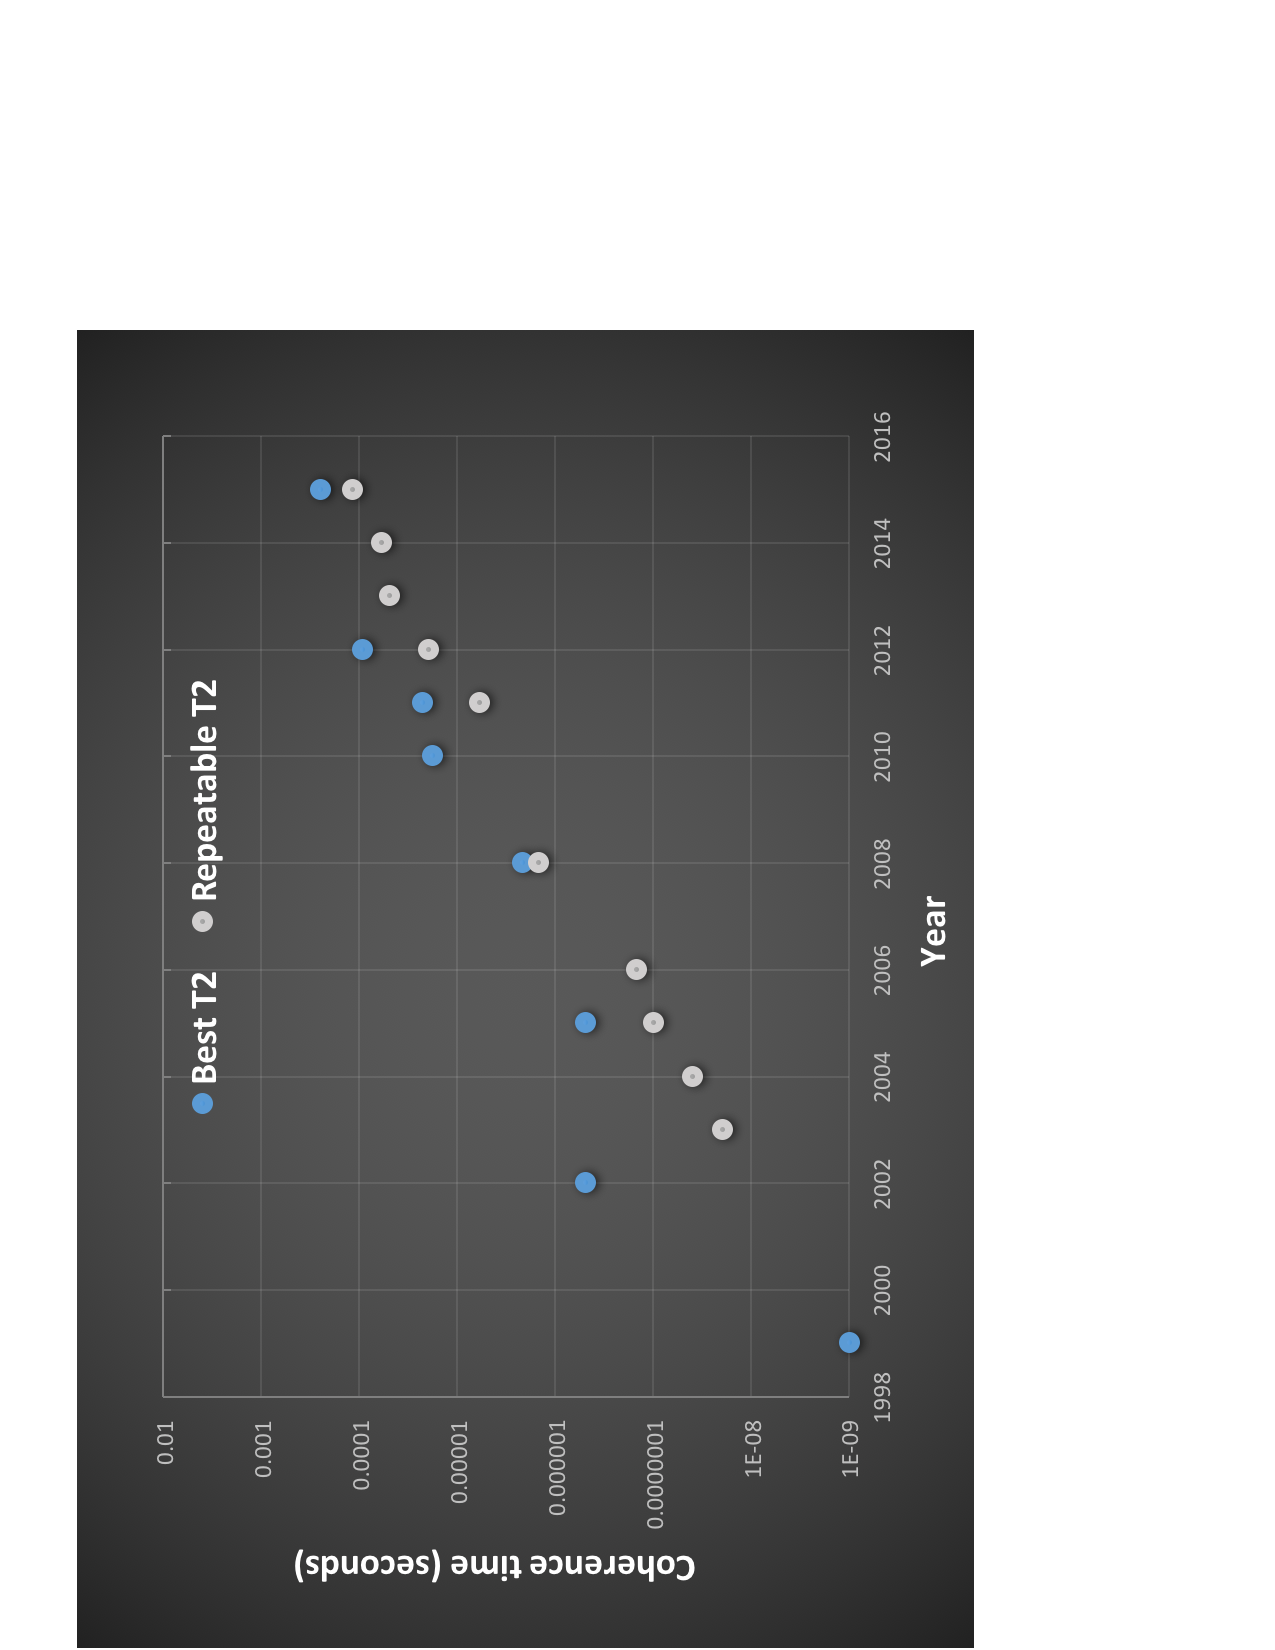
\includegraphics{future/T2h1lc19xmqrdlsor}}}
\caption{Coherence Time Trend}
\label{fig:future:Coherence Time Trend}
\end{figure}

QC 의 발전에 있어서의 또다른 핵심 요소는 decoherence time 입니다.
QC decoherence 는 qubit 들이 불안정하며 시간의 흐름에 따라 붕괴하게 된다는
사실에서 기인합니다.
물론, 이는 전례없는 것은 아닙니다: 무엇보다도, classical computing 의 어디에나
존재하는 dynamic RAM 은 주기적으로 재충전 되어야만 합니다.
하지만, 누군가가 qubit 들을 재충전 할 수 있는 실용적인 방법을 내놓기
전까지는~\cite{GiorgioColangelo2017QC-SpinAngleAmplitude},
decoherence time 을 늘리는 것이 quantum 알고리즘이 더 많은 처리를 할 수 있도록
해줄 겁니다.
Superconducting qubit 을 위한 coherence time 은
Figure~\ref{fig:future:Coherence Time Trend}~\cite{IBM2016QuantumExperience}
에 보인 것처럼 매년 두배가 될겁니다.
이 트렌드를 외삽해 보면 10년 내로 10초의 coherence time 이 가능해 질 것으로, 더
복잡하고 긴시간 동작하는 QC 알고리즘들이 실용적 영역으로 들어올 수 있게 할
것이고 또한 복잡한 error-correction 방법들의 필요를 줄일 것이라 예쌍할 수
있습니다.
\iffalse

Another key element of QC progress is decoherence time.
QC decoherence results from the fact that qubits are fragile, and
decay over time.
Of course, this is not unprecedented: After all, classical computing's
ubiquitous dynamic RAM must be periodically refreshed.
However, until someone comes up with a practical way to refresh
qubits~\cite{GiorgioColangelo2017QC-SpinAngleAmplitude},
increasing decoherence time allows a quantum algorithm to do more
processing.
Coherence time for superconducting qubits seems to be doubling every year,
as shown in
Figure~\ref{fig:future:Coherence Time Trend}~\cite{IBM2016QuantumExperience}.
Extrapolating this trend suggests that 10-second coherence times might
be available in ten years time, which would bring more complex and
long-running QC algorithms into the realm of practicality, and might
also reduce the need for complex error-correction schemes.
\fi

마지막으로, entangle 될 수 있는 qubit 의 갯수 (그리고 entanglement 기간을)
늘리는 것은 Shor's integer-factorization
알고리즘~\cite{Shor:1997:PAP:264393.264406,Kendon:2006:ERS:2011698.2011704} 과
같은 양자 알고리즘들에 중요합니다.
Murphy 의 법칙은 entangle 될 수 있는 qubit 의 갯수를 늘리는 것은 decoherence
time 을 줄일 것이라 이야기 합니다만, 시간이 지나봐야 알 수 있을
겁니다\footnote{
	그래서 여러분은 이 entangle 이 어떻게 동작할지 모르겠나요?
	글쎄요, 어차피 모두 모릅니다~\cite{ScottAaronson2018QuantumInterp}.}

Quantum-state readout 은 더 정확해 질 것이라는 애타는 힌트가
있습니다만~\cite{GiorgioColangelo2017QC-SpinAngleAmplitude}, 이런 기술들이 QC
에 적용될 것인가에 대해서는(sensing 과 분광학에서와는 대조적으로) 확실치
않습니다.
\iffalse

Finally, increasing the number of qubits that can be
entangled (and the duration of the entanglement) is important for
quantum algorithms such as Shor's integer-factorization
algorithm~\cite{Shor:1997:PAP:264393.264406,Kendon:2006:ERS:2011698.2011704}.
Murphy's Law would suggest that increasing the number of qubits that
can be entangled would also decrease decoherence time, but time will
tell.\footnote{
	So you don't understand how entanglement actually functions?
	Well, neither does anyone else~\cite{ScottAaronson2018QuantumInterp}.}

There are some tantalizing hints that quantum-state readout might become
more accurate~\cite{GiorgioColangelo2017QC-SpinAngleAmplitude},
but it is not yet clear that these techniques apply to QC
(as opposed to sensing and spectroscopy).
\fi

연구자들은 최근들어 수십 microkelvins 에서의 gaseous 상태의 3,000 개 rubidium
원자들 entangle 하는데에
성공했습니다만~\cite{RobertMcConnell2015QC-Entangle3000Atoms}, 이게 현재로써는
non-gasuous qubit 집합으로 구성되는 QC 시스템에 어떻게 적용될 수 있을지는
확실치 않습니다.
그러나, 현재의 보고서들은 entanglement 가능성의 합리적인 외삽을 가능하게 할만큼
충분한 데이터를 제공하고 있지 않습니다.\footnote{
	보고서의 문제라기보다는 아마도 편집자의 문제일 가능성이 큽니다.}
QC 에 연관된 추세는 모호해 보입니다.

이런 모든 진보들에도 불구하고, QC 는 다음 섹션의 주제이기도 한 상당한 문제에
직면해 있습니다.
\iffalse

Researchers recently achieved entanglement of 3,000
rubidium atoms in gaseous state at a few tens of
microkelvins~\cite{RobertMcConnell2015QC-Entangle3000Atoms},
though it is unclear how this could be adapted for use in
a QC system, which currently feature highly structured non-gaseous
collections of qubits.
Nevertheless, the current literature does not appear to provide enough
data to permit reasonable extrapolation of entanglement capabilities.\footnote{
	Which is quite possibly the fault of the editor rather than that
	of the literature.}
Trends regarding QC operation times seem to be similarly obscure.

Despite all this progress, QC face significant challenges, which are
the subject of the next section.
\fi

\subsection{Quantum Computing Challenges}
\label{sec:future:Quantum Computing Challenges}

QC 에서의 발전은 흥분되고 보기 좋았습니다만, 이 시스템들은 여전히 관습적
컴퓨팅의 표준에서는 상당히 조잡합니다.
IBM 의 Scott Crowder 가 말했듯, ``1940년대의
반복입니다''~\cite{BradJones2017IBM-QC-Crowder}.
비교를 위해 보자면, 가장 오래된 온전한 컴퓨터인 University of Melbourne 의
1949년도 CSIRAC~\cite{CSIRACMuseumVictoria,CSIRACUniversityMelbourne} 는 1\,KHz
의 코어 클락 주파수로 동작했고, 30\,kW 의 전력을 소모했으며, 3 metric ton 의
무게에, 2,000 개의 진공관 튜브로 구성되었고, 수은 지연선 (Acoustic Mercury
Delay Line) 으로 구현한 768 word 의 RAM 을 가졌습니다.
그리고 마지막의 두가지 요소는 왜 이게 ``운영가능한'' 게 아니라 ``온전한''
것인지에 대한 이유로, 기계적 수은도 600-volt 의 노출된 전선도 2017 년도엔
선호할 만해 보이지 않기 때문입니다.\footnote{
	둘 다 1960년대 초에는 받아들일 만 했습니다.
	2060년대의 주민들은 2017년도의 평범한 실례의 숫자들에 마찬가지로
	끔찍해할 것임에 의심의 여지가 없습니다.}
따라서 한때 CSIRAC 의 메인 메모리로 동작했던 강철관은 수은이 텅빈채이고 전선은
전류를 머금고 있지 않습니다.
더 나아가서, CSIRAC 이후로, 관들은 트랜지스터에 대체되어 구식이 되었고
트랜지스터 역시 결국은 집적회로의 여러 세대들로 인해 구식이 되었습니다.
수은 지연선은 유리 지연선으로 대체되어 구식이 되었고, 유리 지연선은 자기 코어
메모리로, 자기 코어 메모리는 반도체 DRAM 으로 대체되어왔고, DRAM 은 곧
non-volatile RAM (NVRAM) 으로 대체될 것으로 보입니다.
\iffalse


Progress on QC has been exciting and good to see, but these systems are
still quite crude by the standards of conventional computing.
As Scott Crowder of IBM put it,
``It's the 1940s again''~\cite{BradJones2017IBM-QC-Crowder}.
For purposes of comparison, the oldest intact computer, the
University of Melbourne's 1949
CSIRAC~\cite{CSIRACMuseumVictoria,CSIRACUniversityMelbourne},
ran at a core clock frequency of 1\,kHz, consumed 30\,kW of power,
weighs three metric tons,
is constructed of 2,000 vacuum tubes, and has 768 words of RAM
implemented with acoustic mercury delay lines.
And these last are two reasons why it is ``intact'' rather than
``operational'', given that
neither metallic mercury nor exposed 600-volt wiring are
looked upon favorably in 2017.\footnote{
	Both were considered to be perfectly acceptable as late as the
	early 1960s.
	Which is OK.
	The denizens of the 2060s will be no doubt be equally horrified
	by any number of unremarkable 2017 practices.}
The steel tubes that once served as CSIRAC's main memory are therefore
empty of mercury and the wiring is therefore free of current.
Furthermore, since CSIRAC, tubes have been obsoleted by discrete
transistors which were in turn obsoleted by multiple generations of
integrated circuits.
Mercury delay lines were obsoleted by glass delay lines which were
obsoleted by magnetic core memory which were obsoleted by
semiconductor DRAM, which might be on its way to being obsoleted
by non-volatile RAM (NVRAM).
\fi

그러나, CSIRAC 는 처음으로 게임을 하고 음악을 재생할 수 있는 첫번째 컴퓨터였던
것으로 알려져 있습니다.
비슷하게, 우린 미래의 QC 시스템들이 현재의 프로토타입들과는 상당히 다를 것이라
예상할 수 있지만, CSIRAC 와 마찬가지로, 현재의 QC 프로토타입들이 상당한
마일스톤을 찍을 것이라 기대해 볼 수 있습니다.

개선이 필요한 QC 분야를 더 들여다보기 위해,
Section~\ref{sec:future:Programming Model} 는 QC 프로그래밍 모델에 (그리고 일부
영역에 수수께끼를 풀려는 노력으로) 생기는 도전적 문제들을 들여다보고,
Section~\ref{sec:future:Error Rate} 에서는 qubit error rate 을 둘러싼 도전적
문제들을 보고,
Section~\ref{sec:future:Thermodynamics} 에서는 항상 불편한 열역학의 법칙에 의해
생기는 전력 효율성 문제를 이야기하며,
Section~\ref{sec:future:Heuristics} 에서는 고전적 컴퓨터들과 heuristic 의
조합과의 경쟁적 도전사항들에 대해 간략히 알아보고
Section~\ref{sec:future:Quantum Simulation} 에서 고전적 컴퓨터들에서의 QC
시뮬레이션을 알아보고,
Section~\ref{sec:future:Mathematical Advances} 에서는 수학자들로부터 나올 수
있는 경쟁적 도전사항들에 대한 힌트를 알아봅니다.
\iffalse

Nevertheless, the CSIRAC is believed to be the first computer to
play a game and to play music.
Similarly, we should expect future QC systems to look much different
than current prototypes, but we nevertheless have reason to hope that,
like CSIRAC, current QC prototypes will achieve notable milestones.

To shine some light on QC areas needing improvement,
Section~\ref{sec:future:Programming Model} looks at challenges posed by the QC
programming model (and attempts to demystify some aspects),
Section~\ref{sec:future:Error Rate} looks at challenges surrounding qubit
error rates,
Section~\ref{sec:future:Thermodynamics} presents energy-efficiency challenges
posed by the ever-inconvenient Laws of Thermodynamics,
Section~\ref{sec:future:Heuristics} gives an overview of competitive
challenges from the combination of classical computers and heuristics,
Section~\ref{sec:future:Quantum Simulation} looks at simulation of QC
systems on classical computers,
and
Section~\ref{sec:future:Mathematical Advances} hints at possible competitive
challenges from mathematicians.
\fi

\subsubsection{Programming Model}
\label{sec:future:Programming Model}

\begin{figure}[tb]
\centering
\resizebox{2.2in}{!}{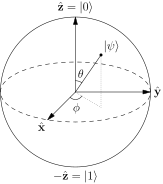
\includegraphics{future/Bloch_Sphere}}
\caption{Qubit as Bloch Sphere}
\label{fig:future:Qubit as Bloch Sphere}
\end{figure}

QC 프로그래밍 모델은 classic-computing 경험을 가진 개발자들을 위해 최대한
맞춰져 있습니다.
이 섹션의 나머지 부분에서는 qubit, quantum entanglement, 그리고 QC 하드웨어와
classic computer 하드웨어 사이의 과계에 대해 다룹니다.
\iffalse

The QC programming model is at best an acquired taste for developers
with classic-computing experience.
The remainder of this section covers qubits,
quantum entanglement,
and
the likely relationship between QC hardware and classic computer hardware.
\fi

\paragraph{Qubit}

Qubit 은 classic-computing 의 bit 과 비슷한 종류의 것인데, 단지 그런 종류일
뿐입니다.
Qubit 의 특성은:
\iffalse

A qubit is sort of like a classic-computing bit, but only sort of.
A qubit is said to:
\fi

\begin{enumerate}
\item	Figure~\ref{fig:future:Qubit as Bloch Sphere} 에 보인 것과 같이, Block
	sphere 로 나타내어집니다.
\item	측정될 때에 0 ($\ket{0}$) 또는 1 ($\ket{1}$) 로 붕괴되는데, 어느 값으로
	붕괴될지에 대한 확률은 $\ket{0}$ 과 $\ket{1}$ 로부터의 상대적 거리를
	Z-축으로 투영한 값의 함수로 계산됩니다.
	따라서, 이 Bloch sphere 의 수식에서의 qubit 은 1 또는 0 으로 측정될
	50\,\% 의 확률을 갖고 있으며, 45\textdegree-북쪽 위도의 qubit 은 1 로
	측정될 확률 14\,\% 와 0 으로 측정될 확률 86\,\% 를 갖습니다.
	이 상황은 기본적으로 개발자들이 sphere 보다는 실선을---또는
	classic-computing bit 을---선호하게 합니다.
\item	(측정 오퍼레이션에 더해서) Bloch sphere 위에서의 순환만을 지원합니다.
\iffalse

\item	Be represented by a Bloch sphere, as shown in
	Figure~\ref{fig:future:Qubit as Bloch Sphere}.
\item	Collapse to a zero ($\ket{0}$) or a one ($\ket{1}$) if measured,
	with probability being a function of the relative distance from
	$\ket{0}$ and $\ket{1}$, but projected onto the Z\=/axis.
	Thus, a qubit on the equator of the Bloch sphere has a 50\,\%
	probability of being measured as a one or as a zero, while
	a qubit on the 45\textdegree-north latitude would have
	a 14\,\% chance of being measured as one and 86\,\% chance
	of being measured as zero.
	This situation naturally causes developers to prefer a line
	segment---or a classic-computing bit---over a sphere.
\item	Support only rotations on the Bloch sphere (in addition to
	the measurement operation).
\fi
\end{enumerate}

Block sphere 의 필요는 주로 현재 qubit 을 나타내는, 물리적 실체들에서 현재
행해질 수 있는 quantum-mechanical 오퍼레이션ㄷ르의 제약인 \#3 에 의한 것입니다.

IBM 의 Quantum Experience 에 의해 지원되는 기본적인 non-entangling
오퍼레이터들은 다음과 같습니다:
\iffalse

It appears that the need for a Bloch sphere is mainly dictated by \#3,
the limitations on the quantum-mechanical operations currently available
on the physical entities that represent qubits.

The basic non-entangling operators supported by IBM's Quantum Experience
are as follows:
\fi

\begin{description}
\item[\qop{H}\,:]
	X-Z 축으로 Block-sphere 를 180\degree{} ($\uppi$ radian), 즉 X-Z 축의
	45\degree{} 선만큼 회전시킵니다.  이는 $\ket{0}$ 를 X-축의 양의 부분이
	Bloch sphere 와 만나는 지점까지 회전시키고, $\ket{1}$ 를 X-축의 음의
	부분이 Bloch sphere 와 만나는 지점까지 회전시킵니다.
	어느 경우든, 우린 50\,\% 1이고 50\,\% 0인 qubit 을 얻게 됩니다.
	\iffalse

	Rotate 180\degree{} ($\uppi$ radians) about the Bloch-sphere
	X-Z axis, that is, about the 45\degree{} line on the
	X-Z plane.  This rotates $\ket{0}$ to the point at which the
	positive X\=/axis intersects the Bloch sphere, and rotates $\ket{1}$
	to the point at which the negative X\=/axis intersects the Bloch
	sphere.
	Either way, we get a qubit that is 50\,\% one and 50\,\% zero.
	\fi
\item[\qop{S}\,:]
	Bloch-sphere 를 Z-축으로 90\degree{} ($\frac{\uppi}{2}$ radian) 만큼
	회전시켜서 $\ket{0}$ 나 $\ket{1}$ 상태의 qubit 에는 아무 변화도
	일으키지 않습니다.
	\iffalse

	Rotate 90\degree{} ($\frac{\uppi}{2}$ radians) about the
	Bloch-sphere Z\=/axis, which has no effect on qubits in the
	$\ket{0}$ or $\ket{1}$ states.
	\fi
\item[\qop{S}$^{\bm{\dagger}}$:]
	Bloch-sphere 를 Z-축으로 $-90\degree$ ($-\frac{\uppi}{2}$ radian) 만큼
	회전시켜서, $\ket{0}$ 나 $\ket{1}$ 상태의 qubit 에는 아무 변화도
	일으키지 않습니다.
	이 오퍼레이터는 \qop{S} 의 반대입니다.
	\iffalse

	Rotate $-90\degree$ ($-\frac{\uppi}{2}$ radians) about the
	Bloch-sphere Z\=/axis, which has no effect on qubits in the
	$\ket{0}$ or $\ket{1}$ states.
	This operator is the inverse of \qop{S}.
	\fi
\item[\qop{T}\,:]
	Bloch-sphere 를 Z-축으로 45\degree{} ($\frac{\uppi}{4}$ radian)
	회전시켜서, $\ket{0}$ 나 $\ket{1}$ 상태의 qubit 에는 아무 변화도
	일으키지 않습니다.
	\iffalse

	Rotate 45\degree{} ($\frac{\uppi}{4}$ radians) about the
	Bloch-sphere Z\=/axis, which has no effect on qubits in the
	$\ket{0}$ or $\ket{1}$ states.
	\fi
\item[\qop{T}$^{\bm{\dagger}}$:]
	Bloch-sphere 를 Z-축으로 $-45\degree{}$ ($-\frac{\uppi}{4}$ radian)
	회전시켜서, $\ket{0}$ 나 $\ket{1}$ 상태의 qubit 에는 아무 변화도
	일으키지 않습니다.
	이 오퍼레이터는 \qop{T} 의 반대입니다.
	\iffalse

	Rotate $-45\degree$ ($-\frac{\uppi}{4}$ radians) about the
	Bloch-sphere Z\=/axis, which has no effect on qubits in the
	$\ket{0}$ or $\ket{1}$ states.
	This operator is the inverse of \qop{T}.
	\fi
\item[\qop{X}\,:]
	Bloch-sphere 를 X-축으로 180\degree{} ($\uppi$ radian) 만큼 회전시켜서
	$\ket{0}$ 를 $\ket{1}$ 로, 그리고 그 반대로도 만듭니다.
	\iffalse

	Rotate 180\degree{} ($\uppi$ radians) about the Bloch-sphere
	X\=/axis, which takes $\ket{0}$ to $\ket{1}$ and vice versa.
	\fi
\item[\qop{Y}\,:]
	Bloch-sphere 를 Y-축으로 180\degree{} ($\uppi$ radian) 회전시켜서 역시
	$\ket{0}$ 를 $\ket{1}$ 로, 그리고 그 반대로도 만듭니다.
	\iffalse

	Rotate 180\degree{} ($\uppi$ radians) about the Bloch-sphere
	Y\=/axis, which also takes $\ket{0}$ to $\ket{1}$ and vice versa.
	\fi
\item[\qop{Z}\,:]
	Bloch-sphere 를 Z-축으로 180\degree{} ($\uppi$ radian) 회전시켜서
	$\ket{0}$ 나 $\ket{1}$ 상태의 qubit 에는 아무 변화도 일으키지 않습니다.
	\iffalse

	Rotate 180\degree{} ($\uppi$ radians) about the Bloch-sphere
	Z\=/axis, which has no effect on qubits in the $\ket{0}$ or
	$\ket{1}$ states.
	\fi
\end{description}

\begin{figure}[tb]
\centering
\resizebox{2.5in}{!}{\rotatebox{270}{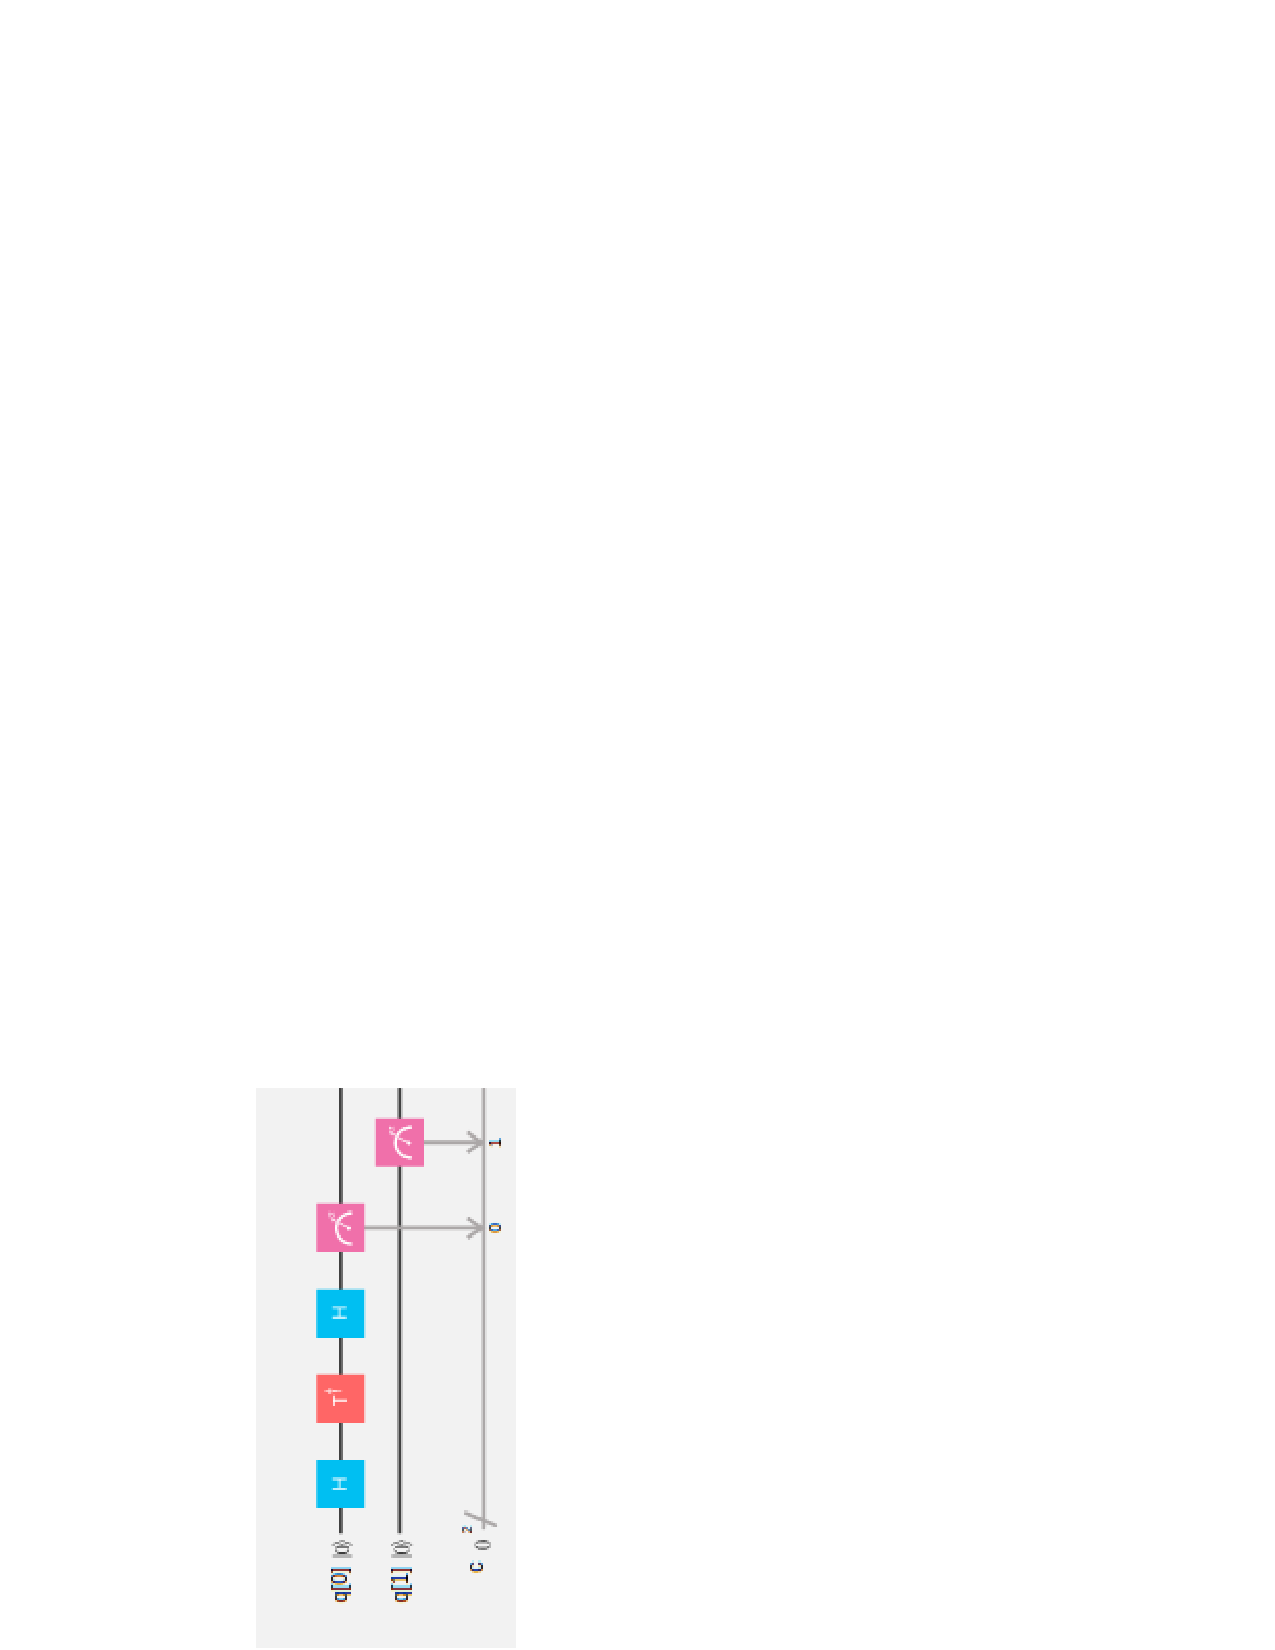
\includegraphics{future/QC-FormConstant.pdf}}}
\caption{QC Program as Quantum Experience Score}
\label{fig:future:QC Program as Quantum Experience Score}
\end{figure}

측정은 qubit z-좌표에 기반해서 1 이나 0 으로 붕괴되도록 만듭니다.
0 으로 붕괴할 확률은 다음과 같습니다:
\iffalse

Measurement causes the qubit to collapse to either one or zero, based
on the z-coordinate of the qubit.
The probability of collapse to zero is:
\fi

\begin{equation}
	\frac{1+z}{2}
\end{equation}

비슷하게, 1 로 붕괴할 확률은 다음과 같습니다:
\iffalse

Similarly, the probability of collapse to one is:
\fi

\begin{equation}
	\frac{1-z}{2}
\end{equation}

따라서, qubit 을 생각하는 한가지 (제한된) 방법은 qubit 을 붕괴 가능성에 기반해
0 과 1 을 포함한 그 사이 값의 소수라고 생각하는 겁니다.
상숟르은 $\ket{0}$ qubit 으로 시작해서 \qop{H}, \qop{S}, 그리고 \qop{T}
오퍼레이션들을 적용하는 것으로 만들어질 수 있습니다.
예를 들어, 상수 $0.14$ 는 \qop{H}, \qop{T}$^\dagger$, 그리고 또다른 \qop{H} 를
$\ket{0}$ qubit 에
Figure~\ref{fig:future:QC Program as Quantum Experience Score} 에 보인 것처럼
적용함으로써 작은 immediate 필드를 갖는 classic 컴퓨터들에서 상수를 만들때와
완전 다르지는 않은 방식으로 만들어질 수 있습니다.
하지만, IBM Q quantum 오퍼레이션들은 50-60~나노세컨드 정도를 소모하므로, 이
오퍼레이션들은 대략 150-180~나노세컨드 정도를 소모할겁니다.
두자리 숫자의 결과를 측정하는데에는 오퍼레이션들이 100 회 정도 반복될 것을
필요로 해서 준비하고 측정하는 시간을 무시하더라도 15-18 마이크로세컨드 정도를
소모할 겁니다.
그만큼의 시간동안, classic-computing floating-point 연산은 10자리 숫자의
정확도로 작은 행렬을 뒤집을 수도 있습니다.

만약 이게 QC 가 제공하는 전부였다면, QC 는 느리고 매우 저품질을 갖는 아날로그
컴퓨터가 되었을 겁니다.
디지털 컴퓨터들은 몇십년 전에 아날로그 컴퓨터를 구식으로 만들었다는 것을 놓고
볼 때, 이 비유는 많은 개발자들이 QC 를 무시하고 그대신 classic-computing
floating point 를 사용하도록 이끌 수 있을 겁니다.
하지만, QC 는 다음 섹션에서 다룰 강력한 기능들을 제공합니다.
\iffalse

Thus, one (limited) way to think of a qubit is as a fixed-point number
ranging between zero and one, inclusive, based on these probabilities
of collapse.
Constants may be formed by starting with (say) a $\ket{0}$ qubit and
applying sequences of \qop{H}, \qop{S}, and \qop{T} operations.
For example, the constant $0.14$ can be formed by applying an
\qop{H}, \qop{T}$^\dagger$, and another \qop{H}
operation on a $\ket{0}$ qubit as shown in
Figure~\ref{fig:future:QC Program as Quantum Experience Score},
in a manner not entirely unlike constant formation on classic
computers with small immediate fields.
However, given that IBM Q quantum operations consume on the
order of 50-60~nanoseconds, this series of operations would
consume around 150-180~nanoseconds.
To measure the result to two digits would require the operation to
be repeated on the order of 100 times, consuming 15-18~microseconds,
ignoring setup and measurement time.
During that time, classic-computing floating-point arithmetic could not
only invert a modest matrix, it could also do so with more than
ten digits of precision.

If this was all that QC provided, QC would be a rather slow and very
low-quality analog computer.
Given that digital computers obsoleted analog computers some decades back,
this analogy might lead many developers to ignore QC and to
use classic-computing floating point instead.
However, QC provides a powerful capability covered in the next section.
\fi

\paragraph{Entanglement}

\begin{figure}[tb]
\centering
\resizebox{3in}{!}{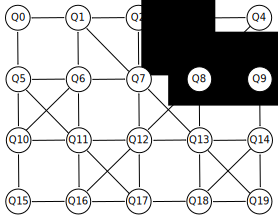
\includegraphics{future/QS1_1}}
\caption{IBM Twenty-Qubit Chip}
\label{fig:future:IBM Twenty-Qubit Chip}
\end{figure}

QC 는 한쌍의 qubit 들을 \emph{entangle} 시키는 \qop{CNOT} 또는
\emph{controlled-NOT} 오퍼레이터를 갖습니다.
\qop{CNOT} 의 다른 사용은 두개의 qubit 들을 Bloch-sphere vector 에 의해 정의된
같은 값, 다른 값, 또는 (대충 말해서) 특정 값들의 조합을 갖도록 만들 수
있습니다.
Entanglement 는 잠재적으로 QC 가 커다란 최적화 문제를 매우 효과적으로 처리할 수
있게 할 수도 있는, entangle 된 변수들 사이의 관계에 제약을 구현하는데에 사용될
수 있습니다.
그러나, 현재의 QC 시스템들은 어떤 qubit 들의 짝이 바로 entangle 될 수 있는지에
대해 제약을 두고 있는데,
Figure~\ref{fig:future:IBM Twenty-Qubit Chip} 에 보인 IBM 의 20-qubit
시스템~\cite{IBMResearch2018QCsystems} 의 토폴로지로 예시화 되어 있습니다.
이 그림에서, 화살표로 연결된 qubit 들은 entangle 될 수 있어서, Q0 는 Q1 과 Q5
와 entangle 될 수 있지만, Q6 와는 entangle 될 수 없습니다.
이 그림에서의 모든 화살표는 양방향입니다만,
Section~\ref{sec:future:Error Rate} 에서 보여지겠지만, 단방향 화살표를 갖는
다이어그램의 QC 시스템도 존재합니다.
\iffalse

QC has the \qop{CNOT} or \emph{controlled-NOT} operator that
\emph{entangles} the pair of qubits operated on.
Different uses of \qop{CNOT} can force the two qubits to have the same
value, opposite values, or other combinations of values (roughly speaking)
defined by a Bloch-sphere vector.
Entanglement can be used to implement constraints
on the relationships of the entangled variables to each other, which
could potentially make QC handle large optimization problems very
efficiently.
That said, current QC systems place constraints on which pairs of
qubits can be directly entangled, as exemplified by the topology
of IBM's 20-qubit system~\cite{IBMResearch2018QCsystems}, which is shown in
Figure~\ref{fig:future:IBM Twenty-Qubit Chip}.
In this figure, qubits connected by arrows can be entangled, so that
Q0 may be entangled with Q1 and Q5, but not with Q6.
All the arrows in this figure are bidirectional, but, as will be seen in
Section~\ref{sec:future:Error Rate},
there are QC systems whose diagrams would have unidirectional arrows.
\fi

여러개의 \qop{CNOT} 오퍼레이션들은 (이론상) 임의의 갯수의 qubit 들을 entangle
할 수 있는데, 이는 서로 다른 요소간의 관계를 표현하는 매우 많은
classic-computing 데이터 구조들을 이 요소들을 나타내는 qubit 들의 entanglement
로 대체할 수 있습니다.
이론 상으로, 이는 계산 복잡도를 상당히 줄일 수 있는데, Shor 의 integer
factorization 을 위한 polynomial-time
algorithm~\cite{Shor:1997:PAP:264393.264406} 이 가장 잘 알려진 예입니다.
실용적으로는, 이런 종류의 계산은 QC 하드웨어에 상당한 개선이 있길 필요로
합니다만, 그런 개선에 대한 기대를 할 이유가
있습니다~\cite{RobertMcConnell2015QC-Entangle3000Atoms}.
많은 개발자들이 QC 프로그래밍 언어의 발전을 희망할 것인데, 예를 들어, 하나의
qubit 에서 하나 이상의 quatum operation 을 하는 언어 요소를 원할 테지만, 현재의
최고 수준의 QC 는 quantum operation 들이 소중하고 주의깊게 절약되어야 한다고
이야기 합니다.
한편, 흰머리가 성성한 우리들은 classic-computing 인스트럭션들과 메모리가
조심스럽게 절약되어야 했던 젊은날의 길었던 시간들에 대한 향수를 느낄수 있을
겁니다.
\iffalse

Multiple \qop{CNOT} operations can (in theory) entangle arbitrarily
large numbers of qubits, which could replace very large numbers of
classic-computing data structures representing relationships between
different entities with entanglement of the qubits
representing these entities.
In theory, this could greatly reduce computational complexity, with
Shor's polynomial-time algorithm for integer
factorization~\cite{Shor:1997:PAP:264393.264406}
being perhaps the best-known example.
In practice, this sort of computation will require substantial
improvements in QC hardware, though there is reason to hope
for such improvement~\cite{RobertMcConnell2015QC-Entangle3000Atoms}.
Many developers might also hope for advances in QC programming languages,
for example, language constructs that do more than a single quantum
operation on a single qubit, however, the current state of the
QC art dictates that quantum operations are precious and must
be carefully conserved.
On the other hand, those of us with ample grey hair might actually
feel a tinge of nostalgia for those long-lost years of our youth when
classic-computing instructions and memory had to be just as carefully
conserved.
\fi

\paragraph{QC as Computational Accelerator}

적은 수의 qubit 들과 그 qubit 들에 사용할 수 있는 제한된 종류의
오퍼레이션들만을 가지고, 현재의 QC 하드웨어는 현대의 운영 체제, 현대의
소프트웨어 스택과 유사한 것은 어떤 것도 돌릴 수가 없을 것이 분명합니다.
Quantum 운영 체제들에 대한 기대가 있음에도 불구하고, QC 하드웨어는 그보다는
GPGPU 나 FPGA 와 유사하게 가속기로 보급될 가능성이
큽니다~\cite{HenryCorriganGibbs2017QCOS}.
이 상황은 이제는 고대의 유물이 되었고 이미 한참 전부터 CPU 칩에 내장된 외장형
인터럽트 컨트롤러, 부동소수점 가속기, 벡터 유닛 등과 비슷한 상황입니다.
반면에, Section~\ref{sec:future:Thermodynamics} 에서 보게 되겠지만, QC
하드웨어가 전통적 CPU 에 내장될 가능성은 별로 없는데, 미래의 QC 하드웨어가 훨씬
높은 온도에서 동작할 수 있게 되기 전까지는 그렇습니다.
\iffalse

Given the small number of qubits and limited types of operations available
on those qubits, current QC hardware is clearly not going to run anything
resembling a modern operating system, let alone a modern software stack.
Instead, QC hardware would more likely be deployed as an accelerator,
similar to a GPGPU or FPGA,
interesting speculation about quantum operating systems
notwithstanding~\cite{HenryCorriganGibbs2017QCOS}.
This situation is similar to the now-ancient external interrupt
controllers, floating-point accelerators, and vector units that have
long since been pulled onto the CPU chip.
In contrast, as we will see in Section~\ref{sec:future:Thermodynamics}, 
it is very unlikely that QC hardware will be pulled into conventional
CPUs, at least not unless future QC hardware runs at much higher
temperatures.
\fi

가까운 미래에, 많은 종류의 QC 연산에 정밀한 한계점들이 존재하게 될겁니다.
많은 문제에 있어서 이것은 괜찮습니다.
무엇보다도 일단 입력 데이터가 두자리 정확도밖에 없다면, 출력 데이터도 두자리
정확도밖에 없더라도 괜찮을 것입니다.
만약 추가적인 정확도가 필요하다면, QC 시스템은 두자리에 대해서 최초 계산을
하고, 이 결과를 classic computation 이 시작하는 데이터로 사용할 수 있게 해줄 수
있을 겁니다.
이는 classic-computing 알고리즘들이 해답에 수렴하는데에는 매우 느리지만 해답
근처까지는 매우 빨리 가는 문제들에 대해서는 매우 유용한 전략임이
증명되었습니다~\cite{JakubKurzak2007MixedPrecision}.
QC 는 classic cimputing 이 너무 느린 영역을 처리하는데에 사용될 수 있을 것이며,
classic computing 은 QC 가 너무 부적합한 영역의 계산에 사용될 수 있을 겁니다.

문제들을 classic computing 과 QC 하드웨어 사이로 나누는 것이 상당한 속도
향상으로 귀결되는 결과가 기대됩니다만, 이게 프로그래밍 모델을 상당히 복잡화
시킨다는 점은 부정할 수 없을 겁니다.
\iffalse

In the near term, there are likely to be strict precision limitations
on many types of QC computations.
For many problems this is OK.
After all if the input data is only precise to two digits, it should
be OK for the output data to be precise to only two digits.
If additional precision is required, the QC system can do the
initial computation to two digits, and this result can be used
as the starting point for a classic computation.
This has proven a useful tactic for problems whose classic-computing
algorithms converge very slowly far from the solution, but very
quickly near the solution~\cite{JakubKurzak2007MixedPrecision}.
QC would be used to handle the portion of the computation for which
classic computing is too slow, and classic computing would be used
for the portion of the computation for which QC is too inaccurate.

It is hoped that splitting the problem over classic computing and
QC hardware will result in great speedups, but there can be no denying
that it greatly complicates the programming model.
\fi

아마도 미래의 어느 시점에서는 QC 시스템으로부터 superposition 과 entanglement
를 포함한 상태를 추출하고 나중에 이를 다시 로딩하는게 가능해질 겁니다.
이게 가능해지기 전까지는, 커다란 QC 시스템을 더 작은 부분들로 나누고 각
부분들은 다른 어플리케이션에 사용되는 경우를 제외하고는, QC 시스템은
context-switch 될 수 없는 특정 목적 전용 가속기일 뿐일겁니다.
물론, 이런 종류의 특정 목적 전용 하드웨어 접근법은 batch 컴퓨팅 모델이 적합한
분야에 있어서는 딱 적합합니다.

QC 에 대해서 더 많은 정보를 원하는 개발자들은 QC 교재들과 IBM 의 Quatum
Experience~\cite{IBM2016QuantumExperience} 을 참조하시기 바랍니다.
QC 와 classic computing 사이의 더 많은 비교는
Section~\ref{sec:future:Heuristics} 과 ~\ref{sec:future:Outlook} 에 있습니다.
\iffalse

Perhaps some time in the future it will be possible to extract
state, including superposition and entanglement, from a QC system,
and then reload it at a later time.
Until this is possible, QC systems are dedicated accelerators
that cannot be context-switched, except perhaps by partitioning
a large QC system into smaller pieces, each piece being used by
a different application.
Of course, these sorts of dedicated-hardware approaches are perfectly
acceptable in situations for which a batch (rather than timesliced)
computing model is suitable.

Developers wishing more information on QC should refer to QC textbooks
and IBM's Quantum Experience~\cite{IBM2016QuantumExperience}.
Additional comparisons between QC and classic computing may be
found in Sections~\ref{sec:future:Heuristics} and~\ref{sec:future:Outlook}.
\fi

\subsubsection{Error Rate}
\label{sec:future:Error Rate}

Quatum effect 는 Heisenberg 의 불확정성
이론~\cite{WeinerHeisenberg1927Uncertain} (또는 덜 알려졌지만 더 놀라운, Bell
의 이론~\cite{JohnSBell1964EPRparadox}) 으로 잘 알려져 있듯이 미묘하고 에러가
발생할 수 있습니다.
따라서 에러 수정 코드가
제안되었습니다~\cite{ADCorcoles2015QuantumErrorDetection}.
다른 연구자들은 QC 에러율을 줄이기 위해 노력하고
있습니다~\cite{PhysRevB.77.180502,PhysRevLett.107.240501,PhysRevLett.111.080502,PhysRevB.86.100506,KristanTemme2016QC-error-mitigation}.
이 연구는 decoherence time 이 100~마이크로세컨드에 근접하는 결과를 내놓았고,
decoherence time 은 Section~\ref{sec:future:Quantum Computing Progress} 에서
논의되었듯 극적으로 증가되고 있습니다.
하지만, 100-마이크로세컨드 decoherence time 이 QC 시스템에 있어서는 놀랍지만
DRAM 에서 일반적으로 명시되는 64-밀리세컨드 refresh time 과 비교하면 전혀
훌륭하지 않습니다.\footnote{
	그리고 이 refresh time 은 보수적으로 잡은 시간입니다. DRAM 은
	일반적으로 1-10~\emph{초} 까지도 충전상태를 유지할 수 있습니다.}
\iffalse

Quantum effects are subtle and subject to errors, as has been
well-known all the way back to
Heisenberg's uncertainty priniciple~\cite{WeinerHeisenberg1927Uncertain}
(or less well-known, but even more mind-bendingly,
Bell's theorem~\cite{JohnSBell1964EPRparadox}).
Error-correcting codes have therefore been
proposed~\cite{ADCorcoles2015QuantumErrorDetection}.
Other researchers are instead working to reduce QC error
rates~\cite{PhysRevB.77.180502,PhysRevLett.107.240501,PhysRevLett.111.080502,PhysRevB.86.100506,KristanTemme2016QC-error-mitigation}.
This work has resulted in decoherence times approaching 100~microseconds,
and decoherence times are increasing dramatically, as discussed in
Section~\ref{sec:future:Quantum Computing Progress}.
However, although a 100-microseconds decoherence time is impressive for
a QC system, it does not look at all good compared to the 64-millisecond
refresh times normally specified for DRAM.\footnote{
	And these refresh times are set conservatively.
	DRAMs can typically hold charge for 1-10~\emph{seconds}.}
\fi

또한, IBM~Q quatum 오퍼레이션들이 50-60~나노세컨드를 소모한다는 걸 놓고 보면,
하나의 qubit 에 대해 이 qubit 이 decohere 하기전까지 행할 수 있는
오퍼레이션들이 많지 않습니다.
예를 들어, 10,000 quantum 오퍼레이션들을 필요로 하는 알고리즘을 하나의 qubit 을
가지고 행하려면 QC 의 수십, 수백배의 발전이 필요합니다.

이 상황은 coherence time 을 늘리기 위한 추가적 연구를 하게 하는 동력이 되었고,
2013년의 한 논문은 coherence time 을 39~\emph{분} 까지 늘려
보였습니다~\cite{KamyarSaeedi2018QC-39-minutes}.
불행히도, 이 연구에 사용된 quantum state 는 atomic nuclei 에 연관되어 있어
상태를 읽고 쓰는데에 여러 nuclear magnetic resonance (NMR) 기계를 필요로 하고,
이 읽기와 쓰기는 액체 헬륨의 온도인 4\,K 에서 행해집니다.
하지만, 읽기와 쓰기사이에, 샘플의 온도는 이 quantum state 에 영향을 끼치지
않고도 연장되 기간동안 실내 온도까지 높여질 수 있습니다.
\iffalse

Furthermore, given that IBM~Q quantum operations consume on the order of
50-60~nanoseconds, it is not possible to carry out very many
operations on a given qubit before it decoheres.
For example, an algorithm requiring 10,000 quantum operations on
a single qubit must wait for order-of-magnitude advances in
the QC state of the art.

This situation should motivate additional research into extending
coherence times, and in fact a 2013 paper demonstrated coherence
times of more than
39~\emph{minutes}~\cite{KamyarSaeedi2018QC-39-minutes}.
Unfortunately, the quantum states used by this work involve atomic nuclei,
which in turn require bulky nuclear magnetic resonance (NMR) machinery
to read and write state, and the reading and the writing takes place
at 4\,K, that is, at the temperature of liquid helium.
However, between reading and writing, the temperature of the sample may
be raised to room temperature for extended periods without affecting
the quantum state.
\fi

이 NMR 요구사항이 많이 나쁘지않다면, 많은 quantum 알고리즘들이 entanglement 를
필요로 합니다~\cite{PeterWSchor2001QuantumAlgorithms}.
불행히도, NMR 시스템들은 nuclear spin 들을 정렬하기 위해 강한 자력장을
사용하며, 우린 한 nucleus 의 과하게 약한 자기장이 근처의 nucleus 에 강력하게
상호작용할 것이라 예상할 수 없으며, 전자구름들과는 더욱 그럴 것이라 예상할 수
없습니다.\footnote{
	Nuclei 의 자기장은 이 nuclear Overhauser 효과를 통해 직접적으로
	상호작용할 수 \emph{있습니다}만~\cite{PhysRev.92.411}, 이 효과는 단순히
	역제곱 법칙을 따르는게 아니라 역육제곱 법칙을 따릅니다!}
지금은 photon 들이 전자 구름들을 쉽게 침투할 수 있는 고에너지 nuclear state
전환을 사용할 수 있습니다.
불행히도, 이런 photon 들은 ``감마선'' 이라고도 불리며, CSIRAC 의
mercury-delay-line 메모리에 사용된 수은으로 채워진 강철 튜브에서 그랬던 것과
같은 정도의 안전성 평판을 갖습니다.
더 나쁜 것은, 이런 감마선은 이 손상을 받는 물질의 결정 격자와 완전히 정렬된
방향으로 가해져야 한다는 것입니다.
긍정적인 면으로는, 이 결정의 반대 방향에 추진력을 빨아들일 수 있는 (그리고
방사능에 안전한) 마법같은 방법이 있다면, 이 방향잡힌 감마선을 많은 공상과학
소설에서 등장하는 감마선 레이저를 만드는데 사용할 수 있을 겁니다.
감마선 레이저는 의심의 여지 없이 무척 나쁜 아이디어지만, 또한 상당히 멋진 나쁜
아이디어이기도 하다는데 반론도 없습니다.\footnote{
	이봐요, 누군가가 cobalt-60 샘플을 가지고 NMR 을 사용해 그 atomic nuclei
	를 완전히 정렬시킨다면 그걸 가지고 무슨 일을
	벌이겠어요!~\cite{1957PhRv..105.1413W}}
\iffalse

If the NMR requirement was not bad enough, many quantum algorithms require
entanglement~\cite{PeterWSchor2001QuantumAlgorithms}.
Unfortunately, NMR systems use strong magnetic fields to align
nuclear spins, and we cannot expect the exceedingly weak magnetic
field of one nucleus to interact strongly with an adjacent nucleus,
especially not with the electron clouds in the way.\footnote{
	The magnetic fields of nuclei \emph{can} interact directly
	via the nuclear Overhauser effect~\cite{PhysRev.92.411},
	but this effect follows not merely the inverse square law,
	but instead an inverse sixth power law!}
Now, it is possible to use higher-energy nuclear state transition,
whose photons are easily able to penetrate electron clouds.
Unfortunately, these photons are also called ``gamma rays'', which enjoy
the same sterling safety reputation enjoyed by the mercury-filled steel
tubes that served as CSIRAC's mercury-delay-line memory.
Worse yet, these gamma rays must be emitted in directions precisely
aligning with the crystal lattice of whatever material is subjected
to this punishment.
On the plus side, given some magical (and radiation-proof) way to absorb
momentum at opposite faces of this crystal, one might use these highly
directional gamma rays to construct the gamma-ray laser that appears in
so many science-fiction stories.
A gamma-ray laser is no doubt an spectacularly bad idea, but there is no
denying that it is also an spectacularly cool bad idea.\footnote{
	Hey, what would happen if someone took a sample of
	cobalt-60 and used an NMR to perfectly align all of its
	atomic nuclei!~\cite{1957PhRv..105.1413W}}
\fi

실수하지 말하야 하는게, 이 39-분의 coherence time 은 상당한 업적입니다만,
nanoscale NMR system~\cite{HJMamin2013QC-nanoscale-NMR} 과 고도로 방향 잡을 수
있고 제어할 수 있는 감마선이 없다면, 이 방법에 기반한 효과적인 컴퓨터를 만드는
것은 상상하기 힘듭니다.

이 극단적인 비실용성은 받아들여지기 어렵고, 상대적으로 따뜻한 운영 온도가
중요한데,
Section~\ref{sec:future:Thermodynamics} 에서 이야기 합니다.
\iffalse

Make no mistake, this 39-minute coherence time is an impressive
achievement, but in the absence
of nanoscale NMR systems~\cite{HJMamin2013QC-nanoscale-NMR} and
highly directional and highly controlled gamma rays, it is
hard to imagine creating an efficient computer based on this approach.
The extreme impracticality notwithstanding, the relatively warm operating
temperatures are important, as discussed in
Section~\ref{sec:future:Thermodynamics}.
\fi

QC 를 위한 nuclear quantum state 의 사용이 공상 과학의 영역에 있는한, 우린 더
불안정한 qubit 들과 에러 교정 기법을 사용해야만 합니다.
한가지 접근법은 여러개의 물리적 qubit 들을 하나의 논리적 qubit 을 표현하는데
사용하고 DRAM 의 것을 연상시키는 형태로 상태를 지속적으로 refresh 해주는
것입니다~\cite{DanielThomasSankPhD}.
Qubit 이 많아지면 에러 발생률은 더 낮아져야만 해서, 수백개의 qubit 을 필요로
하는 알고리즘들에서는 $10^{-8}$ 의 확률의 에러 발생률이
필요합니다~\cite{DanielThomasSankPhD} (비록 일부 QC 연구자들은 $10^{-4}$ 만큼
높은 에러율에도 만족하겠지만요).
\iffalse

As long as use of nuclear quantum states for QC resides in the
realm of science fiction, we must use more fragile qubits
and error correction.
One approach is use of multiple physical qubits to represent
a single logical qubit, continuously refreshing state in an
manner reminiscent of DRAM~\cite{DanielThomasSankPhD}.
The more qubits, the lower the error rate must be, with error
rates on the order of $10^{-8}$ required for algorithms using
a few hundred qubits~\cite{DanielThomasSankPhD} (though some
QC researchers would be satisfied with error rates as high as
$10^{-4}$).
\fi

\begin{figure}[tb]
\centering
\resizebox{3in}{!}{\includegraphics{future/ibmqx2-labeled}}
\caption{IBM Five-Qubit Chip}
\label{fig:future:IBM Five-Qubit Chip}
\end{figure}

\begin{table*}[tbh]
\renewcommand*{\arraystretch}{1.1}
\small
\centering
\subfloat[Single-Qubit Gate Properties]{
\begin{tabular}{@{}ll*{5}{S[table-format=2.3]}@{}}
	\toprule
	& & \multicolumn{5}{c}{Qubit} \\
	\cmidrule{3-7}
	& & \multicolumn{1}{c}{Q\textsubscript{0}} &
		\multicolumn{1}{c}{Q\textsubscript{1}} &
			\multicolumn{1}{c}{Q\textsubscript{2}} &
				\multicolumn{1}{c}{Q\textsubscript{3}} &
					\multicolumn{1}{c@{}}{Q\textsubscript{4}} \\
	\cmidrule(r){1-2} \cmidrule{3-7}
	Qubit Operator & Error Rate (\%) &
	 0.197 &
		 0.129 &
			 0.197 &
				 0.163 &
					 0.094 \\
	& Fidelity (\%) &
	99.803 &
		99.871 &
			99.803 &
				99.837 &
					99.906 \\
	\cmidrule(r){1-2} \cmidrule{3-7}
	Qubit Readout & Error Rate (\%) &
	 4.50 &
		 3.60 &
			 2.00 &
				 1.60 &
					 2.50 \\
	& Fidelity (\%) &
	95.50 &
		96.40 &
			98.00 &
				98.40 &
					97.50 \\
	\bottomrule
\end{tabular}
}

\OneColumnHSpace{-0.15in}%
\subfloat[Multi-Qubit Gate Properties]{
\begin{tabular}{@{}ll*{6}{S[table-format=2.2]}@{}}
	\toprule
	& & \multicolumn{6}{c}{Entanglement Connection} \\
	\cmidrule{3-8}
	& & \multicolumn{1}{c}{CX0\_1} &
			\multicolumn{1}{c}{CX1\_2} &
				\multicolumn{1}{c}{CX0\_2} &
					\multicolumn{1}{c}{CX3\_2} &
						\multicolumn{1}{c}{CX4\_2} &
							\multicolumn{1}{c@{}}{CX3\_4} \\
	\cmidrule(r){1-2} \cmidrule{3-8}
	\multirow{2}{1in}{Qubit Entanglement (\qop{CNOT})} & Error Rate (\%) &
		 3.46 &
			 4.07 &
				 3.26 &
					 2.76 &
						 2.23 &
							 2.66 \\
	& Fidelity (\%) &
		 96.54 &
			95.93 &
				96.74 &
					97.24 &
						97.77 &
							97.34 \\
	\bottomrule
\end{tabular}
}
\caption{Error Rates For IBM Five-Qubit Chip}
\label{tab:future:Error Rates For IBM Five-Qubit Chip}
\end{table*}

불행히도, 현재의 에러율은 그 근처에도 가지 못합니다.
예를 들어,
Figure~\ref{fig:future:IBM Five-Qubit Chip} 에 보인 ``ibmqx2'' 양자 시스템의
경우\footnote{
	2018년 2월 13일 자로 측정된 결과입니다}
qubit 들
(Q\textsubscript{0}, 
Q\textsubscript{1}, 
Q\textsubscript{2}, 
Q\textsubscript{3}, 그리고
Q\textsubscript{4})
그리고 그것들 사이의 entanglement 연결
(CX0\_1,
CX1\_2,
CX0\_2,
CX3\_2,
CX4\_2, 그리고
CX3\_4)
의 에러율이
Table~\ref{tab:future:Error Rates For IBM Five-Qubit Chip} 에 보여진 것과
같습니다.
Gate per-operation fidelity 는 $10^{-4}$ 쓰레스홀드의 10분의 1밖에 되지 않고,
일부 qubit 들은 99.9\% fidelity 를 넘습니다 (이 오퍼레이션들의 리스트를 보려면
Section~\ref{sec:future:Programming Model} 을 참고하세요).
하지만, qubit 의 값을 읽어내는 것은 95\% 에서 98\% 사이 fidelity 에서도 상당히
더 에러에 취약합니다.
이 fidelity 들이 일부 QC 프로그램들을 실행하기에는 충분하겠지만, 앞서 이야기된
희망되는 에러율, $10^{-4}$ 는 너무 먼 목표이고, 이를 달성하기 위해선 상당한
작업과 시간을 필요로 할 겁니다.

Table~\ref{tab:future:Error Rates For IBM Five-Qubit Chip}
에 요약한 시스템은 대칭적이지 않음 역시 알아두시기 바랍니다.
예를 들어, qubit Q\textsubscript{0} 는 qubit Q\textsubscript{1} 과 entangle 될
수 있지만, 그 반대는 아닙니다.

실제로, 2018년 초에 이르러 qubit 을 추가하는건 에러율이 크게 줄지 않는한 QC
능력을 증가시키지 못할 것으로 일부는 믿고
있습니다~\cite{IBMResearch2018QuantumVolume,TheEconomist2018QualityOverQuantity}.
\iffalse

Unfortunately, current error rates are nowhere near either threshold.
For example, for the quantum system ``ibmqx2''\footnote{
	As calibrated on February 13, 2018.}
shown in
Figure~\ref{fig:future:IBM Five-Qubit Chip},
the error rates for the qubits
(Q\textsubscript{0}, 
Q\textsubscript{1}, 
Q\textsubscript{2}, 
Q\textsubscript{3}, and
Q\textsubscript{4})
and the entanglement connections between them
(CX0\_1,
CX1\_2,
CX0\_2,
CX3\_2,
CX4\_2, and
CX3\_4),
are shown in
Table~\ref{tab:future:Error Rates For IBM Five-Qubit Chip}.
The gate per-operation fidelity is only about an order of magnitude
off of the $10^{-4}$ threshold, and some qubits in face exceed 99.9\,\%
fidelity (see Section~\ref{sec:future:Programming Model} for a list of
the operations).
However, reading out the value of a qubit is considerably more
error-prone, with fidelities ranging from 95\,\% to 99\,\%.
Furthermore, entangling a pair of qubits is even more error-prone,
with fidelities ranging from 95\,\% to 98\,\%.
Although these fidelities are sufficient to execute some QC programs, the
aforementioned desired error rates of $10^{-4}$ (let alone $10^{-8}$) are a
long way off, and will likely take considerable work and time to achieve.

Note well that the system summarized in
Table~\ref{tab:future:Error Rates For IBM Five-Qubit Chip}
is not symmetric.
For example, qubit Q\textsubscript{0} can be entangled with
qubit Q\textsubscript{1}, but not vice versa.

In fact, as of early 2018 some believe that adding qubits will not
increase QC capability unless error rates decrease
sharply~\cite{IBMResearch2018QuantumVolume,TheEconomist2018QualityOverQuantity}.
\fi

\subsubsection{Thermodynamics}
\label{sec:future:Thermodynamics}

QC computation 은 열역학적으로 가역적이어고, 매우 적은 열을
발생시킵니다~\cite{Bennett:1973:LRC:1664562.1664568,RichardFeynman1986QuantumMechanicalComputers}.
일 말은 이론적으로, quantum 컴퓨터는 $kT \ln 2$ 의 Landauer
limit~\cite{Landauer:1961:IHG:1661184.1661186} 을 피할 수 있다는 말로, 여기서
$k$ 는 Boltzmann 상수이고 $T$ 는 Kelvin 지수로의 온도입니다.
Boltzmann 상수가 $1.38 \times 10^{-23}$\,J/K 이고, IBM 의 Quantum Experience
하드웨어가 동작하는 오도가 0.015\,K 임을 감안하면 이 한계는 실제로 매우
낮습니다: $1.43 \times 10^{-25}$\,J.

하지만, 그 열역학적 가역성으로 인해, QC 는 그보다도 낮은 한계를 적용받습니다:
\iffalse

QC computation is thermodynamically reversible, generating
very little waste heat~\cite{Bennett:1973:LRC:1664562.1664568,RichardFeynman1986QuantumMechanicalComputers}.
This means that in theory, quantum computers can avoid the
Landauer limit~\cite{Landauer:1961:IHG:1661184.1661186}
of $kT \ln 2$, where $k$ is the Boltzmann constant and $T$ is the
temperature in degrees Kelvin.
Given that the Boltzmann constant is $1.38 \times 10^{-23}$\,J/K,
and given the 0.015\,K operating temperatures that IBM's Quantum Experience
hardware runs at, this limit is indeed low: $1.43 \times 10^{-25}$\,J.

However, because of its thermodynamic reversibiltiy,
QC is governed by an even lower limit:
\fi

\begin{equation}
	\upDelta E \geq \frac{\hbar}{2 \upDelta t}
\end{equation}

여기서 $\upDelta E$ 는 qubit 을 변화시키는데 필요한 에너지를 Joule 단위로
나타낸 것이고, $\upDelta t$ 는 qubit 을 변화시키는데 필요한 시간을 초단위로
나타낸
것이며, $\hbar$ 는 Planck 의 상수로, $6.62 \times 10^{-34}$\,J$\cdot$s 입니다.
IBM 의 Quantum Experience 하드웨어의 50-나노세컨드 스위칭 타임에서, 이 제한은
$5.52 \times 10^{-27}$\,J, 로, Landauer 제한보다 10배 이상 적습니다.

이 두개의 제한들은 모두 놀라울 정도로 작아서, 미친듯이 에너지 효율적인
computation 에 대한 약속을 보장합니다만, 실용적인 면에서는, 일이 그렇게 잘
돌아가지 않습니다.
예를 들어, quantum state 의 초기화와 측정에 의해, 감마 방사선의 이온화에, 열
전도에, 대류에, 그리고 QC 의 실내 온도 방사로 인해, 그리고 quantum error
교정으로 인해, 이 error 교정이 복사된 qubit 들로 구현되는가 아니면 QC
프로그램의 동일한 수행으로 구현되는가에 따라 추가적인 열이 발생할 겁니다.
불행히도, 얼만큼의 열이 발생되는가만이 중요한게 아니고, 이 열이 발생되는 온도
역시 중요합니다.
\iffalse

Here $\upDelta E$ is the energy required to change the qubit in Joules,
$\upDelta t$ is the time taken to change the qubit in seconds, and
$\hbar$ is Planck's constant, which is $6.62 \times 10^{-34}$\,J$\cdot$s.
For the 50-nanosecond switching times of IBM's Quantum Experience
hardware, this limit is $5.52 \times 10^{-27}$\,J, more than an order
of magnitude less than the Landauer limit.

Both of these limits are incredibly small, which holds out the promise
of insanely energy-efficient computation, except that
in practice, things don't work quite so nicely.
For example, additional waste heat will be generated
by initialization and measurement of the quantum state;
by ionizing radiation;
by thermal conduction, convection, and radiation from
the QC's room-temperature surroundings;
and
by the need for quantum error correction, whether that error correction
is implemented by duplicate qubits or by duplicate runs of the QC
program.
Unfortunately, it is not just the amount of heat generated that is
important, but also the temperature at which this heat is generated.
\fi

\newcommand{\TLo}{T_\mathrm{L}}
\newcommand{\THi}{T_\mathrm{H}}
\newcommand{\CPf}{C_\mathrm{P}}

냉장고가 열을 낮은 온도 ($\TLo$) 에서 높은 온도 ($\THi$) 로 이동시키는 능력의
열역학적 온도 한계는 성능의 계수 ($\CPf$) 로 주어집니다:
\iffalse

The thermodynamic theoretical limit on the ability of a refrigerator
to transport heat from a low temperature ($\TLo$) to a high temperature
($\THi$) is given by the coefficient of performance ($\CPf$):
\fi

\begin{equation}
	\CPf = \frac{\TLo}{\THi - \TLo}
\end{equation}

\begin{table}
\rowcolors{1}{}{lightgray}
\renewcommand*{\arraystretch}{1.25}
\centering\footnotesize
\begin{tabular}{p{1.7in}p{0.95in}}
\toprule
Law of Thermodynamics
	& English Translation \\
\midrule
Energy is conserved.
	& Can't win! \\
Entropy increases in closed systems.
	& Can't break even! \\
Entropy approaches a constant value as temperature approaches absolute zero.
	& Can't leave the game! \\
\bottomrule
\end{tabular}
\caption{The Three Laws of Thermodynamics}
\label{tab:future:The Three Laws of Thermodynamics}
\end{table}

이 수식은 도무지 불편한 열역학의 법칙에 연관되어 있으며,
Table~\ref{tab:future:The Three Laws of Thermodynamics} 에 그 관계가 그려져
있습니다.

IBM~Q 를 위한 명목상의 온도는 15~millikelvins 로, 낮은 $\TLo$ 라 이야기 되기
충분할 겁니다.
$\THi$ 가 293\,K (실내 온도) 이고, $\CPf$ 는 $0.000051$ 이라 가정해 봅시다.
이는 곧 $0.000051$~와트의 손실열을 15~millikelvin IBM~Q 로부터 실내온도로
이동시키는데에 냉방기에 \emph{최소한} 1 watt 저력을 필요로 함을 의미합니다.
달리 말해서, 1 watt 의 손실열을 제거하는데 19.5\,kW 가 필요합니다.
따라서,
Section~\ref{sec:future:Quantum Computing Challenges} 에서 CSIRAC 의 3분의
2보다 적은 전력 소모를 이야기했지만, ``매우 작은 손실열'' 은 분명 냉방기를 위해
엄청난 전기요금 고지서를 만들어내고 말겁니다.
또한, 그렇게 커다란 온도 차이에서 데이터를 효율적으로 전송하는 것은 어려운
일입니다.
그러나 이는 여러분의 스마트폰에 IBM~Q 가 들어올 것이라 아직은 상상하기 어려운
두가지 이유에 불과합니다.
이 상황은 또한 현재의 QC 하드웨어가 CPU 칩에 내장될 수 없게 할겁니다---이 냉각
비용은 full-power 칩에서는 금지될 것이며, 낮은 온도에서 동작 가능한 저전력
회로에서조차도 그럴 겁니다.\footnote{
	흥미롭게도, ARM 의 저전력 CPU 들은 칩에 내장된 QC 로 덜 힘든 냉방
	장벽을 마주하게 될겁니다.}
\iffalse

This equation is related to the ever-inconvenient Laws of Thermodynamics,
fancifully illustrated in
Table~\ref{tab:future:The Three Laws of Thermodynamics}.

The nominal temperature for IBM~Q is 15~millikelvins, which certainly
qualifies as a low $\TLo$.
Let's assume $\THi$ is 293\,K (room temperature),
in which case $\CPf$ is $0.000051$.
This in turn means that it requires \emph{at least} one watt of
power into the refrigeration unit to transport $0.000051$~watts
of waste heat from the 15~millikelvin IBM~Q out to room temperature.
Put another way, 19.5\,kW is required to remove one watt of waste heat.
Thus, ``very little waste heat'' can nevertheless generate a significant
power bill for refrigeration, albeit less than two-thirds of the power
consumption of the CSIRAC machine discussed in
Section~\ref{sec:future:Quantum Computing Challenges}.
In addition, efficiently transporting data across such a large
temperature differential can be challenging.
These are but two reasons why you should not expect an IBM~Q in your
smartphone just yet.
This situtation will also prevent current QC hardware from being pulled
onto the CPU chip---the refrigeration costs would be prohibitive for
a full-power chip, even allowing for the lower-power circuitry possible
at low temperatures.\footnote{
	Interestingly enough, ARM's low-power CPU family would face
	a less daunting refrigeration barrier to QC-on-a-chip.}
\fi

\begin{table}
\rowcolors{1}{}{lightgray}
\renewcommand*{\arraystretch}{1.2}
\centering\small
\begin{tabular}{lS[table-format = 3.3]S[table-format = 1.6]S[table-format = 5.1]}
\toprule
Situation
	& \multicolumn{1}{c}{$T$ (K)}
		& \multicolumn{1}{c}{$\CPf$}
			& \multicolumn{1}{r}{\parbox[b]{.75in}{Power per watt\\waste heat (W)}} \\
\midrule
Dry Ice
	& 195
		& 1.990
			& 0.5 \\
Liquid N$_2$
	& 77
		& 0.356
			& 2.8 \\
Liquid H$_2$
	& 20
		& 0.073
			& 13.7 \\
Liquid He
	& 4
		& 0.0138
			& 72.3 \\
IBM~Q	& 0.015
		& 0.000051
			& 19 500.0 \\
\bottomrule
\end{tabular}
\caption{Refrigeration Power Consumption}
\label{tab:future:Refrigeration Power Consumption}
\end{table}

칩에 내장된 QC 로의 장벽을 줄이는 한가지 방법은 QC 의 운영 온도를 높이는 것일
겁니다.
더 높은 온도는
Table~\ref{tab:future:Refrigeration Power Consumption} 에 보인 것처럼
필요한 냉방전력을 극적으로 낮추기 때문에 도움이 됩니다.
따라서, QC 에 사용될 수 있는 높은 온도의 quantum 시스템의 사용은 에너지
효율성을 상당히 개선하고 QC 와의 데이터 전송을 간편하게 해줄겁니다.
불행히도, 현재의 QC 의 수준을 보면, 더 높은 온도는 동시에 coherence time 을
상당히 줄여버릴겁니다.
따라서, 가까운 미래에, QC 시스템은 에너지를 많이 소모하는 냉방기를 필요로 할
것이어서, QC 시스템이 큰 가치를 지닌 킬러 애플리케이션을 필요로 하게 될 겁니다.
\iffalse

One way to reduce the barrier to QC-on-a-chip would be to raise
QC's operating temperature.
Higher temperatures help because the refrigeration power required
decreases dramatically with increasing temperature, as shown in
Table~\ref{tab:future:Refrigeration Power Consumption}.
Therefore, high-temperature quantum systems amenable for QC use would
greatly improve energy efficiency and ease transfer of data to and from
the QC.
Unfortunately, given the current state of the QC art, higher
temperatures also sharply decrease coherence times.
Therefore, for the foreseeable future, QC systems will need
energy-hungry refrigeration systems, which means that QC
systems need a high-value killer app.
\fi

물론, 이 킬러 애플리케이션의 가치가 충분히 높다면, 19.5\,kW 는 저렴한 걸로
생각될 수 있을 겁니다.
이런 경우,
``plenty of room at the bottom''~\cite{RichardPFeynman1959RoomAtBottom} 의
정신에 입각하여, 우리는 더 낮은 온도를 원할 수도 있을 겁니다.
예를 들어, Bose-Einstein condensates
(BECs)~\cite{NIST2001BoseEinsteinCondensate} 는 microkelvin 이하 범위에
위치해서, 흥미로운 대규모 quantum effect 를 보입니다.
이런 응축액 내에 어떻게 컴퓨터를 구성할 것인지도, BEC 로부터의 1 watt 의
손실열을 제거하는데 필요한 1.6\,GW 를 제공할 것인지도 명확치
않습니다---무엇보다도, Emmett Brown 의 공상적인 flux capacitor 도 1.21 gigawatt
만을 필요로 했습니다.
하지만, 물질과 에너지의 저온 상태에 대해서는 탐구해볼 것이 많은데, 그 중 새로운
물질에 대해 하나만 예를 들면
perovskite~\cite{ZhengChen2016PerovskiteQDMOFthinFilm} 이 있습니다.
다른 영역으로는 증가된 기압을 포함해서 diamond avil
cell~\cite{Weir1959DiamondAnvilCell} 은 이제
640\,GPa~\cite{LeonidDubrovinsky2012640GPaDiamondAnvilCell} 에 도달하는데, 이는
지구 중심의 것으로 추측되는 기압의 두배에 가깝습니다.
그런 탐구는 물론 순수한 연구입니다만, QC 가 1940 년애 수준의 개발 단계라면,
순수 연구는 아직 할 역할이 많습니다.

어떤것도 필요한 순수 연구가 아닙니다.
Milli-kelvin 냉각기는 helium-3 를 필요로 하는데, 이는 핵 반응로에서 적은 양만
생성되고 있습니다.
백만-qubit 양자 컴퓨터의 대량 생산은 세계의 helium-3 생산의 상당한 증가를
필요로 할 것이고, 이는 추가적인 핵 반응로를 만들어야 할 것이고, 이는 환경적,
법적, 사회적, 그리고 정치적 영역으로부터 상당한 저항을 받게 될 겁니다.

대안적으로, 실리콘 기반의 qubit 들은 transmon 기반 기기들보다 10배 이상높은
운영 온도의 가능성을 제시합니다만, 이 실리콘 기기들은 현재 73--89\% 의
fieldility 의 높은 entanglement 에러율~\cite{TFWatson2017SiliconQubit} 로
고통받고 있습니다.
하지만, 지금은 실리콘 기기의 초기 단계이므로, 계속 개선될 겁니다.

어떤 방식이든, 킬러 애플리케이션이 분명 필요합니다.
최적화는 그런 킬러 애플리케이션 중 하나가 될 수 있을게 분명합니다만, 다음
섹션에서 보게 되듯이, 여기엔 상당한 경쟁이 있습니다.
\iffalse

Of course, if the value of the killer app is sufficiently high,
19.5\,kW might be considered cheap.
In this case, in the spirit of
``plenty of room at the bottom''~\cite{RichardPFeynman1959RoomAtBottom},
we might want even lower temperatures.
For example, Bose-Einstein condensates
(BECs)~\cite{NIST2001BoseEinsteinCondensate}
form in the sub-microkelvin range, exhibiting interesting
macro-scale quantum effects.
It is not clear how one would construct any sort of computer from
these condensates, nor how one would go about providing the 1.6\,GW
required to remove one watt of waste heat from a BEC---after all,
even Emmett Brown's fictional flux capacitor required only 1.21 gigawatts.
However, much remains to be explored in this realm
of low-temperature exotic states of matter and energy, to say
nothing of new materials, for but one example,
perovskite~\cite{ZhengChen2016PerovskiteQDMOFthinFilm}.
Other avenues include increased pressure, given that diamond anvil
cells~\cite{Weir1959DiamondAnvilCell} can now reach
640\,GPa~\cite{LeonidDubrovinsky2012640GPaDiamondAnvilCell},
which is almost double the estimated pressure at the center of the earth.
Such exploration is of course pure research, but if QC is at 1940s levels
of development, pure research should have a significant role to play.

Nor is pure research all that is required.
Milli-kelvin refrigerators require helium-3, which is currently
produced in small amounts by nuclear reactors.
Mass production of million-qubit quantum computers will require
substantial increases in the world's supply of helium-3, which would
require construction of additional nuclear reactors, which just might face
stiff resistance on environmental, legal, social, and political grounds.

Alternatively, silicon-based qubits offer the prospect of
operating temperatures that are about an order of magnitude higher than
transmon-based devices, but these silicon devices currently suffer from
high entanglement error rates, with fidelities ranging from
73--89\,\%~\cite{TFWatson2017SiliconQubit}.
However, it is early days for silicon devices, so perhaps they will
continue improving.

Either way, a killer app is absolutely necessary.
Optimization might well be one such killer app, but as we will see in the
next section, it has serious competition.
\fi

\subsubsection{Heuristics}
\label{sec:future:Heuristics}

SAT 를 위한 Moore 의 법칙~\cite[Fig.~2.3]{Kroening:2008:DPA:1391237} 은 산업계
수준의 SAT solver 들이 ``수시간'' 내에 1990년대엔 약 100개 변수 정도를 처리하던
수준에서에 2010년엔 1,000,000 개 변수 처리로 진보했으며, 이는 20년 사이에
10000배 증가입니다.
이는 1.5년마다 두배를 의미하며, 이는 현재도 진행중입니다.
예를 들어, 2016년에, 한 소프트웨어 검증 어플리케이션은 84시간동안 90,000,000 개
변수들을 처리했습니다~\cite{LihaoLiang2016VerifyTreeRCU}.
다른 곳에서도 비슷한 폭발적 진보가
있었습니다~\cite{SharadMalik2010SATSolverHistory,SATCompetition2002,vanHarmelen:2007:HKR:1557461,Malik:2009:BST:1536616.1536637,JamesEzick2014ExtremeSAT}.
이 진보는 SAT-solver heuristic 에서의 상당한 진보
덕입니다~\cite{Kroening:2008:DPA:1391237,Zhang:2002:QEB:647771.734434,SharadMalik2010SATSolverHistory,Malik:2009:BST:1536616.1536637,Audemard:2009:PLC:1661445.1661509}.
\iffalse

Moore's Law for SAT~\cite[Fig.~2.3]{Kroening:2008:DPA:1391237} shows
that industrial-strength SAT solvers have advanced from handling
``in a few hours'' about
100 variables in 1990 to handling about 1,000,000 in 2010, an increase
of four orders of magnitude in 20 years.
This represents a doubling every 1.5 years, and this progress has
continued.
For example, in 2016, a software-verification application solved a
90,000,000-variable problem in 84 hours~\cite{LihaoLiang2016VerifyTreeRCU}.
Others have noted similar exponential
progress~\cite{SharadMalik2010SATSolverHistory,SATCompetition2002,vanHarmelen:2007:HKR:1557461,Malik:2009:BST:1536616.1536637,JamesEzick2014ExtremeSAT}.
This progress has been due to great advances in SAT-solver
heuristics~\cite{Kroening:2008:DPA:1391237,Zhang:2002:QEB:647771.734434,SharadMalik2010SATSolverHistory,Malik:2009:BST:1536616.1536637,Audemard:2009:PLC:1661445.1661509}.
\fi

Heuristic 으로 해결되지 않은 특수한 SAT 케이스들 (아마 가장 유명한건 pigeonhole
principle 의 어플리케이션을 필요로 하는
것들~\cite[page~38]{Kroening:2008:DPA:1391237} 일겁니다) 이 존재하긴 합니다만,
지속적인 진보를 가정하는데에는 문제가 없는듯 합니다.
그리고 다른 복잡한 문제들에도 비슷한 진보가
이뤄져왔습니다~\cite{WikipediaPrimalityTest,WikipediaTSP,WikipediaIntegerFactorization}.
논리적, 하드웨어/소프트웨어 검증, 전자적 배치, 그리고 SAT 나 다른 어려운
문제들을 줄이는 것들을 개선하는데에 거대한 경제적 가치가 있음을 생각하면 이는
놀라운 일이 아닙니다.
이 가치는 이 영역에서 상당한 연구와 개발을 지속시킬 것으로 예상될 수 있으며,
추가적인 머신러닝 작업도 포함될 수 있을
겁니다~\cite{ShaiHaim2009SAT-MachineLearning}.
예를 들어, 머신러닝 테크닉은 필요에 의해 대안적 해결책이 적용될 수 있는 다른
경우들을 허용할 겁니다.
\iffalse

Although there are special SAT cases that have not yet succumbed to
heuristics, perhaps most famously those requiring application of the
pigeonhole principle~\cite[page~38]{Kroening:2008:DPA:1391237},
it seems safe to assume continued progress.
And similar progress has also been achieved for other hard
problems~\cite{WikipediaPrimalityTest,WikipediaTSP,WikipediaIntegerFactorization}.
This should not be surprising, given that there is great economic value
in improving logistics, hardware/software verification, electronic layout,
and other problems that reduce to SAT or to other famous hard problems.
This value can be expected to continue to drive significant research
and development in this area, perhaps incorporating additional
machine-learning work~\cite{ShaiHaim2009SAT-MachineLearning}.
For example, perhaps machine-learning techniques will allow difficult
cases to be detected so that alternative solution methods can be applied
as needed.
\fi

물론, 이런 작업의 대부분은 heuristic 과/또는 probabilistic 이었고, 따라서
이것들을 QC 알고리즘들과 비교하는건 일단은 부당해 보일 수 있습니다.
하지만, QC 알고리즘들은 본질적으로 그 에러 발생률과 측정의 불확정성으로 인해
probabilistic 하며, 따라서 이 비교는 사실 상당히 공정합니다.
매우 일반적인 classical 싱글 쓰레드 SAT solver 들로 최근에 해결된
문제들~\cite{LihaoLiang2016VerifyTreeRCU} 을 해결하기 위해선 90,000,000 qubit
들이 필요하다는 점을 놓고 보면 이는 주류 QC 에 상당한 도전입니다.

이런 고려는 또한 완전히 이론적이지도 않습니다.
특정 알고리즘을 위한 classical 소프트웨어에 비교해서 D-Wave 머신의 10,000 배의
성능 향상이 문서화된 일이 있습니다~\cite{McGeoch:2013:EEA:2482767.2482797}.
이 일은 언론에도 알려진 많은 것들의 상당한 압축적
문서화입니다~\cite{CharlesChoi2013D-WaveGoogleNASA}.
하지만, 또다른 연구자는 desktop-class 시스템에서 싱글쓰레드로 돌아가는
classical 소프트웨어가 D-Wave 하드웨어보다 10,000 배의 성능적 우위를 보일 수
있음을
보였습니다~\cite{AlexSelby2014D-Wave-vs-classical,AlexSelby2013D-WaveHarderQUBO}.
여전히 다른 연구자들은 특정 문제들에 대한 D-Wave 하드웨어의 quantum 속도향상의
증거를 찾지 못했습니다, D-Wave 하드웨어가 그런 속도향상을 보이는 다른 문제들도
있긴 하지만
말입니다~\cite{AdrianCho2014QC-D-WaveNoSpeedup,TroelsFRonnow2014QC-D-WaveNoSpeedup}.
놀라울 수도 있겠지만, 한 D-Wave 연구자는 quantum 속도향상을 찾는 것 자체가 어떤
면에선 문제가 있다고
주장합니다만~\cite{MohammadHAmin2015QC-D-Wave-QuantumSpeedupProblematic}, QC
시스템 성능을 측정하는 것은 실제 간단하지 않은 것으로
보입니다~\cite{PhysRevLett.118.100601,ArsTechnica2017QC-SpeedTradeoffs}.
\iffalse

Of course, much of this work has been heuristic and/or probabilistic,
so it might at first glance seem unfair to compare them to
QC algorithms.
However, QC algorithms are inherently probabilistic due to error rates
and measurement uncertainties, so the comparison is in fact eminently
fair.
This could be a severe challenge to mainstream QC, given the potential
need for 90,000,000 qubits to address problems recently solved by
very ordinary classical single-threaded SAT
solvers~\cite{LihaoLiang2016VerifyTreeRCU}.

Nor are these considerations solely theoretical.
There has been work documenting a four-orders-of-magnitude
performance advantage of D-Wave machines compared to classical
software for certain algorithms~\cite{McGeoch:2013:EEA:2482767.2482797}.
This work achieved considerable traction in the popular
press~\cite{CharlesChoi2013D-WaveGoogleNASA}.
However, another researcher has shown that classical software running
single-threaded on desktop-class systems can
have four-order-of-magnitude performance advantages over
D-Wave hardware~\cite{AlexSelby2014D-Wave-vs-classical,AlexSelby2013D-WaveHarderQUBO}.
Still other researchers found no evidence of quantum speedup
from D-Wave hardware for selected problems, though there might well be
other problems for which D-Wave hardware produces such
speedups~\cite{AdrianCho2014QC-D-WaveNoSpeedup,TroelsFRonnow2014QC-D-WaveNoSpeedup}.
Perhaps surprisingly, a D-Wave researcher argues that the search for
quantum speedup is in some sense
problematic~\cite{MohammadHAmin2015QC-D-Wave-QuantumSpeedupProblematic},
however, it really does appear that evaluating QC system performance is
not at all
trivial~\cite{PhysRevLett.118.100601,ArsTechnica2017QC-SpeedTradeoffs}.
\fi

하지만, SAT solver 들을 위한 pigeonhole principle 과 같은 hard-problem
heuristics 의 한계들~\cite[page~38]{Kroening:2008:DPA:1391237} 은 언젠가 높은
가치를 갖는 QC 킬러 애플리케이션이 나타나기를 바라는 바램을 갖게 합니다.

불행히도, heuristic 들만이 QC 시스템의 활용에 대한 위협은 아닙니다.
고전적 컴퓨팅 시스템들은 QC 시스템을 시뮬레이션 하는데에 숙련되어 있다고
증명되어 있는데, 이에 대해 다음 섹션에서 알아봅니다.
\iffalse

Nevertheless, limitations in hard-problem heuristics such as the
pigeonhole principle for SAT
solvers~\cite[page~38]{Kroening:2008:DPA:1391237}
provides some hope that a high-value QC killer app might someday emerge.

Unfortunately, heuristics are not the only threat to the utility
of QC systems.
Classical computing systems are proving reasonably adept at simulating
QC systems, as described in the next section.
\fi

\subsubsection{Quantum Simulation}
\label{sec:future:Quantum Simulation}

IBM 의 Quantum Experience~\cite{IBM2016QuantumExperience} 는 2016년부터
클라우드 기반의 QC 시스템의 고전적 컴퓨팅을 사용한 시뮬레이션을 제공했으며, IBM
은 최근 자신의 QC-시뮬레이션 게임을 50개 qubit 까지
늘렸습니다~\cite{WillKnight2017IBM50qubitSim}.
고전적 컴퓨팅의 QC 시스템 시뮬레이션 능력이 QC 시스템 자체의 발전을 앞지르는
것도 가능할까요?

고전적 컴퓨팅은 좋은 싸움을 이끌어낼 수 있겠지만, QC 시스템을 시뮬레이션 하는
것은 여전히 qubit 갯수에 있어
기하급수적입니다~\cite{ScottAaronson2017IBM50qubitSim}.
앞서 이야기한 50개 qubit 시뮬레이션이 하는 일은 CPU 시간을 메모리와 교환하는
것으로, 적은 메모리도 아니고, 3.0 과 4.5\,TB 사이입니다.
따라서 50개 qubit QC 시스템을 시뮬레이션 하는 것은 상당히 인상적이지만,
대부분의 사람들이 가까운 시간내에 각자의 스마트폰에서 수행할만한 일은 아닙니다.
\iffalse

IBM's Quantum Experience~\cite{IBM2016QuantumExperience}
has provided a cloud-based classical-computing simulation of
QC systems since 2016, and IBM has recently raised its
QC-simulation game to 50 qubits~\cite{WillKnight2017IBM50qubitSim}.
Is it possible that classical computing's ability to simulate
QC systems will outpace the capabilities of the QC systems themselves?

Although classical computing does seem to be putting up a good fight,
simulating a QC system is still exponential in the number of
qubits~\cite{ScottAaronson2017IBM50qubitSim}.
What the 50-qubit simulation does is trade CPU time for memory, and not
just a little memory, but rather between 3.0 and 4.5\,TB of it.
So although simulating a 50-qubit QC system is quite impressive,
it is not something that most people will be
running on their smartphones any time soon.
\fi

그러나, 추가적인 QC 시뮬레이션 발전이 있을 가능성은 큽니다.
이는 정말 흥미로운 경주가 될겁니다!

수학의 발전이 또다른 잠재적 위협이 될 수 있는데, 다음 섹션에서 이에 대해
살펴봅니다.
\iffalse

That said, it is quite possible that additional QC simulation advances
are in the offing.
It is truly an exciting race to be watching!

Advances in mathematics might also be a potent threat, as we will see
in the next section.
\fi

\subsubsection{Mathematical Advances}
\label{sec:future:Mathematical Advances}

QC 에서 더욱 기대를 돋우는 전망 중 하나는 Shor's polynomial-time integer
factorization
알고리즘~\cite{Shor:1997:PAP:264393.264406,WikipediaShorsAlgorithm} 으로, 작은
정수를 위한 버전이 연구실에서
구현되었습니다~\cite{LievenMKVandersypen2001ShorQFactoring}.
하지만, 현재의 polynomial-factoring 알고리즘은 하찮지 않습니다.
예를 들어, \co{maxima} 프로그램은 x86 싱글쓰레드 랩탑에서 20초 내에 59 자리
숫자를 인수분해\footnote{
	\scriptsize
	63698321299468802831035558537099113360211126822411635339497 는
	15780285428767, 15780285428771, 그리고
	255798667878176814448339699861021 의 곱입니다.}
할 수 있습니다.
물론, 이는 RSA 를 깨기 위해 인수분해 해야하는 1,000 자리 정수에 비하면 매우
작은 숫자이고, 인수분해가 지수적이라면 RSA 는 상당히 안전합니다.
\iffalse


One of the more tantalizing promises of QC is Shor's
polynomial-time integer factorization
algorithm~\cite{Shor:1997:PAP:264393.264406,WikipediaShorsAlgorithm},
which has been implemented in the lab for small
integers~\cite{LievenMKVandersypen2001ShorQFactoring}.
However, current polynomial-factoring algorithms are not
inconsequential.
For example, the \co{maxima} program can factor a 59-digit number\footnote{
	\scriptsize
	63698321299468802831035558537099113360211126822411635339497,
	which is the product of 15780285428767, 15780285428771, and
	255798667878176814448339699861021.}
in less than 20 seconds single-threaded on an x86 laptop.
Of course, this is a very small number compared to the 1,000-digit
integers that would need to be factored in order to break RSA,
and if integer factorization is exponential, RSA is quite safe.
\fi

하지만, unexpected classic-computer polynomial-time integer primality 테스트가
최근에
증명되었습니다~\cite{ManindraAgrawal2004PrimesIsInP,WikipediaAKSPrimalityTest}.
이제 classic-computer polynomial-time integer factorization 알고리즘이 그 뒤를
따르리라 누가 말하지 못하겠습니까?

어려운 문제에 대한 수학적 해결책의 가능성을 무시하기는 쉽습니다.
이런 경향에 굴복하는 걸 막는 한가지 방법은 지난 50 년간의 주요한 진보들의
목록을 고려해 보는 겁니다.
\iffalse

However, an unexpected classic-computer
polynomial-time integer primality test was recently
devised~\cite{ManindraAgrawal2004PrimesIsInP,WikipediaAKSPrimalityTest}.
Who is to say that a classic-computer polynomial-time integer
factorization algorithm won't soon follow?

It is all too easy to dismiss the possibility of mathematical solutions
to hard problems.
One way to avoid succumbing to this temptation is to consider the
long list of major advances over the last 50 years:
\fi

\begin{description}
\item[1970:] Hilbert's 10\textsuperscript{th} problem 이 풀릴 수 없음을 증명.
\item[1975:] Fractal.
\item[1976:] Four-color problem 의 증명.
\item[1984:] Linear programming problem 을 풀기 위한 첫번째 polynomial-time
	     알고리즘 등장.
\item[1994:] Fermat's Last Theorem 증명.
\item[1998:] Kepler's conjecture 증명.
\item[2002:] Polynomial-time integer primality 테스트.
\item[2002:] Catalan's conjecture 증명.
\item[2003:] Poincar\'e conjecture 증명.
\item[2004:] classification of finite simple groups 증명.
\item[2013:] 한정된 수로 차별되는 소수의 짝의 값에는 값의 한계가 없다는 것에
	     대한 증명.
\item[2015:] Graph isomorphism problem 에의 quasi-polynomial time solution.
\iffalse

\item[1970:] Proof that Hilbert's 10\textsuperscript{th} problem
	is unsolvable.
\item[1975:] Fractals.
\item[1976:] Proof of the four-color problem.
\item[1984:] First polynomial-time algorithm for solving linear
	programming problems.
\item[1994:] Proof of Fermat's Last Theorem.
\item[1998:] Proof of Kepler's conjecture.
\item[2002:] Polynomial-time integer primality test.
\item[2002:] Proof of Catalan's conjecture.
\item[2003:] Proof of the Poincar\'e conjecture.
\item[2004:] Proof of the classification of finite simple groups.
\item[2013:] Proof that there is no bound on the values of
	pairs of primes differing by a finite number.
\item[2015:] Quasi-polynomial time solution to the graph isomorphism
	problem.
\fi
\end{description}

이 문제들 중 여럿은 여러 세기동안 존재했으며, 그 중 가장 유명한건 Fermat's Last
THeorem 일겁니다.
2013년의 prime-pair 결과는 Euclid 의 기원전 300년의 twin-prime hypothesis 로의
중요한 한걸음 진전을 의미하는데, 이는 2천년 이상의 기간동안 이루어진 중요한
한걸음 진전이라고도 말할 수 있겠습니다.

아마도 한편에서는 수학의 어려운 문제들을 해결하려는 경쟁이 존재하고 다른 쪽에는
완벽한 large-scale quantum computing 을 위한 경쟁이 존재합니다.
만약 그렇다면, 우린 이 두개의 방법 사이의 경쟁이 거기 관련된 모두를 위해 좋은
일일 것이라 생각해 볼 수 있을 겁니다.
다음 섹션은 Classical computing 대비 QC 의 현재의 경쟁적 위치에 기반한 전망을
살펴봅니다.
\iffalse

Several of these problems had stood for centuries, perhaps most famously
Fermat's Last Theorem.
The 2013 prime-pair result represents the first significant step forward
on Euclid's 300BC twin-prime hypothesis, that is to say, the first
significant step forward in more than two millennia.

Perhaps there is a race to solve hard problems in mathematics on
the one hand and to perfect large-scale quantum computing on
the other.
If so, we can hope that the competition between these two approaches
will be good for all concerned.
The next section assesses QC's outlook based on its current
competitive position with respect to classical computing.
\fi

\subsection{Outlook}
\label{sec:future:Outlook}

그래서, QC 가 세계를 집어삼키기 위해선 뭐가 필요할까요?

이 섹션은 이 질문에 대해 두가지 측면을 살펴봅니다:
(1)~``제품 품질 QC 시스템을 만들기 위해선 뭐가 필요할까?'' 와
(2)~``QC 킬러 어플리케이션은 무엇일까?''
\iffalse

So what is required for QC to take over the world?

This section looks at two aspects of this question:
(1)~``What is needed to make a production-quality QC system?'' and
(2)~``What is the QC killer app?''
\fi

\subsubsection{Production-Quality QC Systems}
\label{sec:future:Production-Quality QC Systems}

산업계에서 사용될만한 QC 시스템은 $10^{-8}$ 아래의, 가능하다면 더 낮은 qubit 당
에러 발생률을 필요로 합니다.
Shor 의 알고리즘은 이런 qubit 이 굉장히 많이 entangle 될 것을 필요로 하고 또한
수천개의 범용적 qubit 들을 필요로 하빈다.
Classsical SAT solver 들을 이기기 위해서는 수백만 qubit 이 필요할 겁니다.
높은 대역폭과 낮은 응답시간으로 QC 시스템에 데이터를 넣고 뺄 수 있어야만
합니다.
QC 시스템의 전력 소모 (냉각장치 포함) 는 풀려 하는 문제의 값어치에 상응해야만
하며, 또한 같은 문제를 푸는 classical computing 시스템의 것과 경쟁할 만한
수준이어야만 합니다.
\iffalse

An industrial-strength QC system requires per-qubit error rates below the
$10^{-8}$ threshold, preferably far below.
Shor's algorithm requires that a great many of these qubits be entangled,
and also requires several thousand general-purpose qubits.
Beating classical SAT solvers will require many millions of qubits.
It must be possible to load data into and extract results from QC
systems with high bandwidth and low latency.
The power consumption of a QC system (including refrigeration) must be
commensurate with the value of the problem being solved, and must also
be competitive with classical computing systems solving the same problem.
\fi

언젠가는, QC 시스템의 전체 능력에 대한 측정이 필요할 겁니다.
그런 한가지 후보는
\emph{Quantum volume}~\cite{LevSBishop2017QuantumVolume,TaliaGershon2017QuantumVolume} 의
개념으로, qubit 들의 수, decoherence 까지의 오퍼레이션들의 수, 연결성, 병렬성,
그리고 에러율 등을 포함합니다.
다른 기술들에서의 기존 경험은 더 많은 측정들이 제안될 것을 이야기합니다.
여러 QC 킬러 어플리케이션들이 나타나야 하고, 그것들은 해당 어플리케이션의
필요사항들에 맞춰진 특수한 측정이 있게 될겁니다.

물론, 그런 특수화는 실제로 킬러 어플리케이션이 있을 것을 필요로 하는데, 이에
대해서는 다음 섹션에서 이야기합니다.
\iffalse

At some point, an agreed-upon measure of the overall capability of a
QC system will be needed.
One early candidate is the concept of
\emph{quantum volume}~\cite{LevSBishop2017QuantumVolume,TaliaGershon2017QuantumVolume},
which incorporates number of qubits, number of operations until decoherence,
connectivity, parallelism, and error rate.
Past experience with other technologies indicates that quite a few more
measures will be proposed, with some being more self-serving than others.
Should multiple QC killer apps appear, it is likely that specialized
measures will be tuned to the requirements of a given app.

Of course, such specialization requires that there actually be killer
apps, which leads to the next section.
\fi

\subsubsection{QC Killer Apps}
\label{sec:future:QC Killer Apps}

이 섹션은 다섯개의 잠재적 QC 킬러 어플리케이션인,
Simon's periodicity problem,
Shor's integer factorization algorithm,
Grover's search algorithm,
quantum mechanical dynamics,
optimization problems, 그리고
gaming 에 대해 평가해 봅니다.
\iffalse

This section evaluates five potential QC killer apps,
Simon's periodicity problem,
Shor's integer factorization algorithm,
Grover's search algorithm,
quantum mechanical dynamics,
optimization problems, and
gaming.
\fi

\paragraph{Simon's Periodicity Problem}
\label{sec:future:Simon's Periodicity Problem}

Shor~\cite{PeterWSchor2001QuantumAlgorithms} 에서 설명된대로, Simon's problem
은 함수의 주기성에 대한 계산을 필요로 합니다.
이 문제를 풀기 위한 polynomial-time classical 알고리즘이 없다고 가정해 봅시다.
이렇게 되면 질문은 ``이 문제를 푸는게 왜 가치있는가?'' 가 됩니다.
현재로써는, 별도로 고려된 Shor's algorithm 을 제외하고는 이 알고리즘을 가치있게
사용한 예가 알려진 바 없습니다.
\iffalse

Simon's problem, as described by
Shor~\cite{PeterWSchor2001QuantumAlgorithms},
requires computing the periodicity of a function.
Let's assume that there is no polynomial-time classical
algorithm solving this problem.
The question then becomes ``Why is solving this problem valuable?''
At present, there is no known valuable use for this algorithm,
other than Shor's algorithm, which is considered separately.
\fi

\paragraph{Shor's Integer Factorization Algorithm}
\label{sec:future:Shor's Integer Factorization Algorithm}

Shor's algorithm 은 정수들을 polynomial time 내에 인수분해 합니다.
이 결과는 (백해무익하지 않다면) 상당히 가치있습니다만, 현재의 QC 시스템은 RSA
암호화를 깨는데 필요한 수천 자리 숫자들에 Shor's algorithm 을 수행하지도
못합니다.
이 알고리즘은 범용의 상당히 entangle 된 qubit 들을 필요로 하며, 따라서 우리는
2017년 5월의 IBM~Q 의 16개 qubit 시스템으로부터 시작해야만 합니다.
D-Wave 의 1.4~년당 규모가 두배가 되는 경험을 가정해 보면, QC 시스템이 오늘날의
RSA 를 깨는데 걸리는 시간은 13년 정도로 가정해 볼 수 있습니다.
한편으로는, IBM 이 8개월당 규모가 두배가 되는 경험을 가정해 보면, RSA 는 5년
내로 깨어질 것입니다.
물론, 두 경우 모두 QC 시스템이
Section~\ref{sec:future:Quantum Computing Challenges} 에서 이야기되는 도전들을
해결할 수 있다는 가정 아래입니다.
더 나아가서, Shor's algorithm 의 진짜 구현은 대략 1억개의 추가적인 qubit 들이
필요할 것이어서~\cite{RachelCourtland2017GoogleQC}, RSA 의 수명을 훨씬 연장시킬
듯 보입니다.

하지만, 더도 아니고 덜도 아니고, 살짝만 편집증적인 사람들이라도 RSA 를
교체한다는 식의 생각을 하기에 너무 이르지는 않다고 느낄 겁니다.\footnote{
	다른 한편, 오늘날의 RSA 로 암호화된 것으로 분류되는 정보는 QC 가 암호를
	풀어낼 수 있게 되기 전에 다른 부류로 분류될 겁니다.}
\iffalse

Shor's algorithm factors integers in polynomial time.
This result would be quite valuable (if rather destructive),
but current QC systems are nowhere near able to run
Shor's algorithm on the thousand-digit numbers required
to break RSA cryptography.
This algorithm requires general-purpose highly entangled qubits,
so we must start with IBM~Q's May 2017 sixteen-qubit system.
Assuming D-Wave's 1.4~years per doubling, it will be about thirteen
years before QC systems can break current-day RSA.
% 1000 digits is about 1000*l(10)/l(2)=3322 bits
% Assume 1 qubit per bit for Shor's algorithm.
% At D-Wave doubling rate: 1.4*l(3322/16)/l(2)=13.1 years
On the other hand, if IBM sustains its 8-month doubling time, RSA has
less than five years to live.
% IBM from 5 to 16 qubits in a year: l(2)/l(16/5)=.59592202035757028109 years
% This is 12*l(2)/l(16/5)=7.15 months.
% So at IBM doubling rate: 0.5959*l(3322/16)/l(2)=4.6 years.
Of course, both cases assume that QC surmounts the challenges called
out in Section~\ref{sec:future:Quantum Computing Challenges}.
Furthermore, it seems likely that a real implementation of Shor's
algorithms would need additional qubits, as in about one hundred
million of them~\cite{RachelCourtland2017GoogleQC},
which would significantly extend RSA's lifespan.

Nevertheless, even those who are only slightly paranoid might consider
it to be not too early to start thinking in terms of replacing RSA.\footnote{
	On the other hand, present-day classified information encrypted
	using RSA might well be declassified long before QC is able
	decrypt it.}
\fi

\paragraph{Grover's Search Algorithm}
\label{sec:future:Grover's Search Algorithm}

Grover's algorithm 은 $N$ 항목의 순서잡히지 않은 리스트를 $\O{\sqrt N}$ 시간
안에 찾아냅니다.
이것은 데이터를 통해 탐색을 하는 것과 반대로 해법들을 위해 암묵적 탐색을 하기
위해 의도되었습니다.
왜 그런지 보기 위해, 어떤 데이터가 탐색될 수 있기 전에, 그 데이터 리스트는 QC
시스템에 먼저 다운로드 되어야만 하고, 이 다운로드는 데이터 항목들의 수가 $n$
이라고 할 때 $\O{n}$ 계산 복잡도를 가질 것이란 점을 생각해 보세요.
여기에 대해 경쟁자인 classical system 은 이 시간을 데이터를 정렬하거나 데이터
상에 어떤 인덱스를 구성하거나 하면서 사용할 수 있고, 이런 동작들의 계산
복잡도는 $\O(n \log_2 n)$ 이며, classical system 은 이 탐색을 $\O{\log N}$ 시간
동안 수행할 수 있는데, 이는 Grover's algorithm 에서 약속하는 $\O{\sqrt N}$
시간보다 훨씬 빠른 것입니다.
\iffalse

Grover's algorithm searches an unordered list of $N$ items
in $\O{\sqrt N}$ time.
This is mainly intended for implicit search for solutions as opposed
to searching through data.
To see why, keep in mind that before any data can be searched,
that data list must be downloaded into the QC system, and that
this download will have computational complexity $\O{n}$, where
$n$ is the number of data items.
The competing classical system can use this time to sort the data
or to construct any desired index over the data, and the computational
complexity of these operations can be considered to be $\O{n \log_2 n}$,
after which the classical
system can carry out the search in $\O{\log N}$ time, which
is much faster than the $\O{\sqrt N}$ time promised by
Grover's algorithm.
\fi

\QuickQuiz{}
	classic-computing 의 정렬/인덱싱에 $\O{n}$ 이 걸리고 classic-computing
	탐색에 $\O{n \log_2 n}$ 이 걸린다니 이게 무슨 말이죠?
	해시 테이블에서는 $\O{n}$ 과 $\O{1}$ 이면 되는데요!
	\iffalse

	What do you mean $\O{n}$ for classic-computing sorting/indexing
	and $\O{n \log_2 n}$ for classic-computing search?
	Hash tables do $\O{n}$ and $\O{1}$ respectively!!!
	\fi
\QuickQuizAnswer{
	고정된 크기 해시 테이블의 탐색은 $\O{n}$ 이지, $\O{1}$ 이 아닙니다.
	그리고 해시 테이블의 크기를 재조정하기 위해서는, 공정성이 크기 재조정이
	올바르게 수행되는데 걸리는 오버헤드를 지시합니다.

	그렇지만, 제대로 튜닝된 고정크기 해시 테이블에서의 예는 특정 상황에서는
	적합하고, 왜 이 섹션의 점근적 분석이 quantum computing 에 전혀
	불공정하지 않은지를 잘 보입니다.
	\iffalse

	Fixed-size hash table lookups are $\O{n}$, not $\O{1}$.
	And for a resizing hash table, fairness dictates that the overhead
	of resizing be properly accounted for.

	That said, the example of a properly tuned fixed-size hash table
	is entirely appropriate for specific situations, and clearly
	illustrates why this section's asymptotic analysis is not at
	all unfair to quantum computing.
	\fi
} \QuickQuizEnd

$m$ 개의 탐색들이 있다면, Grover's algorithm 에서의 전체 계산 복잡도는 다음과
같이 계산됩니다:
\iffalse

If there are to be $m$ searches, then the overall computational
complexity of Grover's algorithm is given by:
\fi

\begin{equation}
	n + m \sqrt n
\end{equation}

비슷하게, classical computing 에서는:
\iffalse

Similarly, for classical computing:
\fi

\begin{equation}
	\left( n + m \right) \log_2 n
\end{equation}

더 큰 숫자들에서는 classical computing 에서의 승리를 의미하는 비율 계산을
해보면:
\iffalse

Forming the ratio, so that larger numbers indicate a win for classical
computing:
\fi

\begin{equation}
	\frac{n + m \sqrt n}{\left( n + m \right) \log_2 n}
\label{eq:Grover to Classic Overhead Ratio}
\end{equation}

물론, 누군가는 $n$ 과 $m$ 을 각 방법에 걸맞게 선택할 수도 있습니다.
하지만 작은 $m$ 을 선택하는건 말이 안되는데, 이 경우에는 단순한 $O(n)$ 순차적
스캔이 승자가 될 것이기 때문입니다.
더 흥미로운 시나리오들은 더 큰 값의 $m$ 을 사용합니다.

첫번째 시나리오는 더 큰 $n$ 과 $m$ 을 위한
Equation~\ref{eq:Grover to Classic Overhead Ratio}
을 살펴봅니다.
일단 $m$ 이 증가함에 따른 극한을 취함으로써 단순화 시켜봅시다:
\iffalse

Of course, one can pick $n$ and $m$ to favor either approach.
It makes little sense to choose small $m$ because the winner of that
race is a simple $\O{n}$ sequential scan.
More interesting scenarios use larger values of $m$.

The first scenario looks at
Equation~\ref{eq:Grover to Classic Overhead Ratio}
for large $n$ and $m$.
Let's keep life simple by first taking the limit as $m$ increases:
\fi

\begin{equation}
	\lim_{m\to\infty} \frac{n + m \sqrt n}{\left( n + m \right) \log_2 n}
	\Rightarrow \frac{\sqrt n}{\log_2 n}
\label{eq:sqrt n by log 2 n}
\end{equation}

이어서, $n$ 증가에 따라 이 한계를 적용해 보면:
\iffalse

Next, we take the limit as $n$ increases:
\fi

\begin{equation}
	\lim_{n\to\infty} \frac{\sqrt n}{\log_2 n}
	\Rightarrow \frac{\log 2}{2} \sqrt n
\end{equation}

이는 한계 없이 증가해서, 매우 커다란 데이터 셋에 대해 매우 많은 횟수의 탐색을
하게 되는건 classical computing 에서 하는게 나을 것을 의미합니다.

두번째 시나리오는 데이터셋이 크지만, 데이터셋의 일부분 $p$ 만큼만 탐색된다고 해봅시다.
따라서 우린 $m = pn$ 을
Equation~\ref{eq:Grover to Classic Overhead Ratio} 에 대입시킬 수 있습니다:
\iffalse

This increases without limit, indicating the very large numbers of searches
over very large data sets favors classical computing.

The second scenario assumes that the dataset is large, but that only
some fraction $p$ of the dataset is searched for.
We therefore substitute $m = pn$ into
Equation~\ref{eq:Grover to Classic Overhead Ratio}:
\fi

\begin{equation}
	\frac{n + p n \sqrt n}{\left( 1 + p \right) n \log_2 n}
\end{equation}

$n$ 을 취소시키면:
\iffalse

Canceling $n$:
\fi

\begin{equation}
	\frac{1 + p \sqrt n}{\left( 1 + p \right) \log_2 n}
\end{equation}

우린 점근적 동작에 관심있으므로, 분자에서 $1$ 을 무시할 수 있고, $p$ 를
취소시키면, 다음 결과가 나옵니다:
\iffalse

Because we are interested in asymptotic behavior, we can ignore the
$1$ in the numerator, then cancel $p$, resulting in:
\fi

\begin{equation}
	\frac{\sqrt n}{\log_2 n}
\end{equation}

이는 Equation~\ref{eq:sqrt n by log 2 n} 과 같은 것이므로, 이 역시 classical
computing 에서가 더 낫습니다.

Grover's algorithm 이 좋게 보이게 하기 위한 마지막 시도로, 세번째 시나리오는
데이터셋은 크지만, 탐색되는 부분은 $m = n^\alpha$ 로 주어진다고 해봅시다.
이를
Equation~\ref{eq:Grover to Classic Overhead Ratio}
에 대입해 보면:
\iffalse

This is the same as Equation~\ref{eq:sqrt n by log 2 n},
so this arrangement also favors classical computing.

In a final attempt to show Grover's algorithm in a good light,
the third scenario assumes that the dataset is large, but that the portion
searched is given by $m = n^\alpha$.
Substituting into
Equation~\ref{eq:Grover to Classic Overhead Ratio}:
\fi

\begin{equation}
	\frac{n + n^\alpha \sqrt n}{\left( n + n^\alpha \right) \log_2 n}
\end{equation}

간략화 시키면:
\iffalse

Simplifying:
\fi

\begin{equation}
	\frac{n + n^{\alpha + \frac{1}{2}}}{\left( n + n^\alpha \right) \log_2 n}
\end{equation}

분자와 분모의 점근적 동작은 $\alpha$ 의 값에 의존적입니다.
분모에 대해서는 (Grover 오버헤드):
\iffalse

The asymptotic behavior of the numerator and denominator depend on
the value of $\alpha$.
For the numerator (Grover overhead):
\fi

\begin{eqnarray}
	\alpha \leq \frac{1}{2} & \Rightarrow & n \\
	\alpha > \frac{1}{2} & \Rightarrow & n^{\alpha + \frac{1}{2}}
\end{eqnarray}

분자에 대해서는 (classical-computing 오버헤드):
\iffalse

For the denominator (classical-computing overhead):
\fi

\begin{eqnarray}
	\alpha \leq 1 & \Rightarrow & n \log_2 n \\
	\alpha > 1 & \Rightarrow & n^\alpha \log_2 n
\end{eqnarray}

첫번째 범위는 $\alpha \leq \frac{1}{2}$ 로, 그 비율이 다음과 같습니다:
\iffalse

The first range is $\alpha \leq \frac{1}{2}$, where the ratio is as follows:
\fi

\begin{equation}
	\frac{n}{n \log_2 n} = \frac{1}{\log_2 n}
\end{equation}

그리고 우린 마침내 Grover's algorithm 이 더 나은 영역을 찾았습니다!
이는 $m = p^\alpha$ 의 천천히 커지는 값은 classical computing 에게 훨씬 나은
초기화 시간 계산 복잡도를 이겨내기 충분할 만큼 많은 탐색을 제공하지 않기
때문입니다.

두번째 영역은 $\frac{1}{2} < \alpha \leq 1$ 로, 비율은 다음과 같습니다:
\iffalse

And we finally have a regime that favors Grover's algorithm!
The reason is that the slowly growing value of $m = p^\alpha$ does
not give classical computing enough searches to make up for its
greater initialization-time computational complexity.

The second range is $\frac{1}{2} < \alpha \leq 1$,
where the ratio is as follows:
\fi

\begin{equation}
	\frac{n^{\alpha + \frac{1}{2}}}{n \log_2 n} =
	\frac{n^{\alpha - \frac{1}{2}}}{\log_2 n}
\end{equation}

$\alpha > \frac{1}{2}$ 이고 당연하게도 $n \geq 1$ 임을 우린 알고 있기에, 이
결과는
Equation~\ref{eq:sqrt n by log 2 n} 아래로 한정되어서 이 영역에서도 classical
computing 이 더 나을 것임을 알 수 있습니다.
이는 classical computing 의 더 큰 초기화 시간 계산 복잡도를 무효화 할만큼
충분한 양의 탐색이 주어지기 때문입니다.

마지막 영역은 $\alpha > 1$ 인 곳으로, 여기서의 비율은 다음과 같습니다:
\iffalse

Because we know $\alpha > \frac{1}{2}$ and of course $n \geq 1$,
we know that this result is bounded below by
Equation~\ref{eq:sqrt n by log 2 n}, so that this range again
favors classical computing.
The reason is that there are enough searches to make up for
classical computing's greater initialization-time computational
complexity.

The final range is $\alpha > 1$, where the ratio is as follows:
\fi

\begin{equation}
	\frac{n^{\alpha + \frac{1}{2}}}{n^\alpha \log_2 n}
\end{equation}

$n^\alpha$ 를 생략시키면:
\iffalse

Cancelling $n^\alpha$ yields:
\fi

\begin{equation}
	\frac{\sqrt n}{\log_2 n}
\end{equation}

이는 정확히
Equation~\ref{eq:sqrt n by log 2 n} 으로, $\frac{1}{2} < \alpha \leq 1$
영역만큼은 아니지만 이 영역에서도 classical computing 이 나을 겁니다.

Classical computing 의 더 큰 초기화 시간 계산 복잡도를 극복할 만큼 충분한
탐색이 존재하는 한, classical computing 은 Grover's algorithm 을 이깁니다.

그렇다곤 하나, 이 분석은 일부 한계가 있습니다:
\iffalse

This is exactly
Equation~\ref{eq:sqrt n by log 2 n}, so that this range again
favors classical computing, though interestingly enough not by
as much as the 
$\frac{1}{2} < \alpha \leq 1$ range.

As long as there are enough searches to overcome classical computing's
greater initialization-time computational complexity, classical computing
beats Grover's algorithm.

That said, this analysis has some limitations:
\fi

\begin{enumerate}
\item	명시적인 리스트가 가정되었습니다.
	암묵적 리스트는 quantum computing 을 더 선호할 수도 있습니다.
\item	전통적인 정렬과 인덱싱은 classic-computing 탐색에서의 전통적인 $O(\log
	N)$ 계산 복잡도로 가정되었습니다.
\item	Quantum computing 은 매우 커다란 데이터 셋을 처리할 수 있을 것이라
	가정되었습니다.
\item	모든 quantum error 교정 은 상수의 오버헤드를 일으킬 것으로
	가정되었습니다.
\item	데이터는 classical-computing 시스템에 저장되어 있습니다.
	만약 전체 데이터셋이 quantum computer 에 저장되어 있을 수 있다면 이
	분석은 크게 바뀔 겁니다.
\iffalse

\item	Explicit lists are assumed.
	Implicit lists might well favor quantum computing.
\item	Traditional sorting and indexing is assumed to result in
	the traditional $\O{\log N}$ computational complexity for
	classic-computing search.
\item	Quantum computing is assumed to be capable of handling
	very large data sets.
\item	Any required quantum error correction is assumed to incur
	constant overhead.
\item	The data is stored on classical-computing systems.
	The analysis changes dramatically if the full dataset
	can be stored in the quantum computer.
\fi
\end{enumerate}

그러나, $n$ 개 항목의 데이터 셋에서, $\sqrt n$ 이나 그보다 적은 것들만이
탐색된다면 Grover's algorithm 이 점진적으로 널리 사용될 것이라는 법칙을 만들어
냅니다.

다시 말하지만, 많은 사람들이 Grover's algorithm 이 문제를 최적화 하기 위한
해법의 탐색을 보함해 더 많은 일반적 탐색들에 더 잘 적용될 수 있을 것이라 믿고
있습니다.
QC 를 통한 최적화는 이 섹션의 뒤에서 이야기 합니다.
\iffalse

Nevertheless, it does produce the useful rule of thumb that Grover's
algorithm can asymptotically prevail if, for a dataset of $n$ items,
$\sqrt n$ or fewer of them will be searched.

Again, most believe that Grover's algorithm would be better applied to
more general searches, including searching for solutions to optimization
problems.
Optimization via QC is taken up later in this section.
\fi

\paragraph{Quantum Mechanical Dynamics}
\label{sec:future:Quantum Mechanical Dynamics}

Quantum mechanical dynamics 의 시뮬레이션.
QC 시스템들은 그 자신들을 classical system 들이 QC 시스템들을 시뮬레이션 할 수
있는 것보다 기하급수적으로 빠르게 시뮬레이션 할 수 있을 것이라
믿어졌습니다~\cite{Feynman1982}.
하지만, 제조 가능한 QC 시스템들에 근본적인 기하학적 한계는 classical 시스템들이
제조에 덜 친화적인 기하학의 quantum 시스템들을 효과적으로 시뮬레이션할 기회가
있을 것이라 이야기 합니다.
그러나 Microsoft 는 quantum chemistry 가 재구성 가능한 QC 하드웨어에 기반한
최초의 QC 킬러 어플리케이션이 될 것이라
이야기합니다~\cite{TomSimonite2017QC-MS-Chemistry}.
Microsoft 만이 아닙니다: 중국의 연구자들은 QC 를 quantum photon interaction 을
모델하는데에 적용하려 노력하고 있습니다~\cite{StephenChen2017ChinaQC}.
Google 은 molecular hydrogen 을 모델링하기 위해 2-qubit 시스템을
사용했고~\cite{RichardChirgwin2016GoogleQC}, molecule 을 QC 코드로 변환하는
컴파일러를 만들고 있습니다~\cite{RichardChirgwin2017GoogleQC}.
또한, IBM 은 molecular hydrogen 만이 아니라 LiH 와 BeH\textsubscript{2} 를 6개
qubit 들로 모델링 했습니다.
IBM 은 50-qubit 시스템을 사용해서 유력한 아이디어의 증명을 할 수 있을 것으로
기대하고 있습니다.
\iffalse

Simulating quantum mechanical dynamics.
It is believed that QC systems will be able to simulate themselves
exponentially faster than classical systems will be able to
simulate QC systems~\cite{Feynman1982}.
However, the geometric constraints inherent in manufacturable
QC systems suggests that classical systems have a chance
to efficiently simulate quantum systems with less
manufacturing-friendly geometries.
Microsoft is nevertheless betting on quantum chemistry as being
the initial QC killer app~\cite{TomSimonite2017QC-MS-Chemistry},
perhaps based on reconfigurable QC hardware.
Nor is Microsoft alone: Chinese researchers are working to apply
QC to model quantum photon interactions~\cite{StephenChen2017ChinaQC}.
Google used a two-qubit system to model molecular
hydrogen~\cite{RichardChirgwin2016GoogleQC} and is working on a
compiler to translate from molecules to QC
code~\cite{RichardChirgwin2017GoogleQC}.
In addition, IBM modeled not only molecular hydrogen, but also
LiH and BeH\textsubscript{2} using up to six qubits.
IBM expects to deliver a more convincing proof of concept using a
50-qubit system.
\fi

어느 경우든, quantum chemistry 가 Schr\"{o}dinger's equation 을 풀 것을 필요로
해서 gigabyte 크기의 sparse matrix 들의 역행렬을 구할 수 있을 것을 필요로
한다는 점을 놓고 보면, 이 영역에서의 진보는 상당히 가치있을 것입니다.
\url{https://fold.it} 에서의 긍정적 경험을 놓고 보면, QC 의 경쟁자 중 하나는
기계 학습이 될 수 있습니다.
Molecules 자신이 또다른 경쟁자가 될 가능성도
있습니다~\cite{Chin-wenChou2017ManipulateMolecule}, 현재까지 이 방법은 매우
작은 molecule 들로만 제한되긴 하지만요.
하지만 molecule 자신을 사용하는 모든것은 정의에 의해 물리 화학이고, classical
computing 을 quantum mechanical dynamics 에 적용하는 큰 이유는 비용을 줄이고
결과를 더 빨리 얻으려는 것이었음을 언급해둘 가치가 있습니다.
\iffalse

In any case, given that quantum chemistry requires solving
Schr\"{o}dinger's equation, which in turn can require inverting
gigabyte-sized sparse matrices, progress in this area would
be quite valuable.
One of QC's competitors might be machine learning, given the positive
experiences with \url{https://fold.it}.
It is also possible that another competitor might turn out to be the
molecules themselves~\cite{Chin-wenChou2017ManipulateMolecule}, though
currently these methods are restricted to very small molecules.
But it is worth noting that anything using the molecules themselves
is by definition physical chemistry, and the big reason for applying
classical computing to the quantum mechanical dynamics was to reduce
cost and obtain results more quickly.
\fi

물론, 물리 화학과 classic computing 의 창조적 결합은 더 나은
결과를 낼 수도 있을 건데, ``그럴 수도 있다'' 이긴 합니다.
예를 들어, 최근의 한 발전은 얼음의 non-crystalline glass phase, 극단적으로 낮은
온도, 그리고 향상된 scanning tunneling electron microscope 을 사용해서 많은
단백질의 원자 단위 이미지를 생성합니다.
이 발전은 그 발명자에게 2017년 노벨
화학상~\cite{NobelPrizeChemistry2017,JohnTimmer2017ChemistryNobel}을
안겼습니다.
그러나, 이 기술은 극단적 조건 하에서의 특정 부류의 분자들에만 적용되어서, QC 의
가치를 증명할 여지를 많이 남겨둡니다.
\iffalse

Of course, innovative combinations of physical chemistry and
classical computing might well produce even better results,
although a key word here is ``might''.
For example, one recent advance employs a non-crystalline glass phase
of water ice, extremely low temperatures, and an improved scanning
tunneling electron microscope to create atomic-scale images of
large proteins.
This advance garnered its inventors the 2017 Nobel Prize in
Chemistry~\cite{NobelPrizeChemistry2017,JohnTimmer2017ChemistryNobel},
and for good reason.
Nevertheless, this technique is specialized to certain types of molecules
in extreme conditions, leaving considerable scope for QC to prove
its worth.
\fi

고전적 컴퓨팅의 영역에 닿지 않을 수 있는 다른 문제들이 있는데, quantum thermal
Hall conductance 의 시뮬레이션과 같은 것입니다.
불행히도, 그런 문제들은 quantum computing 의 영역 바깥이기도
합니다~\cite{ZoharRingel2017QuantizedGravityHall,RichardChirwin2017ThermalHallConductance}.

따라서, quantum chemistry 는 여전히 QC 의 최고의 킬러 앱이 될 수 있을 겁니다.
\iffalse

There are other problems that are provably out of the reach of
classical computing, such as simulating quantum thermal Hall conductance.
Unfortunately, such problems are also provably out of the reach of
quantum computing~\cite{ZoharRingel2017QuantizedGravityHall,RichardChirwin2017ThermalHallConductance}.

Thus, quantum chemistry might still be QC's best killer-app bet.
\fi

\paragraph{Optimization Problems}
\label{sec:future:Optimization Problems}

앞의 섹션들은 D-Wave 의 최적화 문제에서 타겟으로 하고 있는 시장을 이야기
했습니다.
SAT 를 풀기 위한 QC 알고리즘은 변수당 하나의 qubit 만을 필요로 할 것이며,
D-Wave 가 qubit 의 갯수를 매 1.4년마다 두배로 늘려가는 것을 지속한다고
가정하면, D-Wave 기계가 Liang's SAT-based Linux-kernel RCU correctness
proof~\cite{LihaoLiang2016VerifyTreeRCU} 를 재현하는데 35년이 걸립니다.
\iffalse

Earlier sections have discussed D-Wave's target market of optimization
problems.
Assuming that a QC algorithm for solving SAT requires only one qubit
per variable, and assuming that D-Wave continues doubling qubits every
1.4 years, it will be 35 years before a D-Wave machine can reproduce
Liang's SAT-based Linux-kernel RCU correctness
proof~\cite{LihaoLiang2016VerifyTreeRCU}.
\fi

유명한 Traveling Salesman Problemv(TSP) 에의 개선된 해결책은 물류상의 비용 (과
환경적 효과) 을 줄이는데 있어 상당히 가치있을 것입니다만, 현재의 classic
heuristic 들은 수백개의 도시에 대해서 최적에 가까운
답~\cite{Martin:1992:LMC:2307953.2308141} 을 찾을 수 있으며 임의의 많은 수의
도시들에 대해서 최적의 것보다 40\,\% 이상 길지 않은 루트를 찾을 것을 보장하는
polynomial-time 알고리즘들~\cite{Sebo:2014:STN:2688265.2688281} 은, 수십년 전의
50\,\% bound 에 비해
개선되었습니다~\cite{NicosChristofides1976TSP-FiftyPercent}.
2006년에 이르러 TSP solver 들은 85,900개 도시 문제에 최적의 답을
찾아냈습니다~\cite{DLApplegate2007TSPtextbook}.
도시당 하나의 qubit 을 가정하고 D-Wave 가 시스템 상의 qubit 의 갯수를 1.4년마다
두배씩 늘려가는 것을 지속한다고 가정할 때, 이 문제를 해결할 수 있는 D-Wave
시스템을 만드는데에는 7년 이상이 걸립니다.
하지만, (도시마다가 아니라) 도로 부분마다 하나의 qubit 이 필요해질 가능성이
있어보이고, 이 경우 훨씬 더 많은 qubit 이 필요해질 것이어서, 실은 매우 많은
시간을 기다려야 하게 될겁니다.

물론, SAP 과 TSP 를 위한 수많은 classical-computing heuristic 에 커다란 노력이
있었습니다.
덜 익숙한 문제에 대해선, QC 가 더 나은 결과를 제공할 수
겁니다~\cite{JohnPreskill2018NISQ}

Quantum computing 이 언젠가는 이 경주에서 승리하게 될 수 있겠습니다만,
classic-computing heuristic 이 인상적인 경쟁을 보일 것임에도 의심의 여지가
없습니다.
\iffalse

Improved solutions to the famous Traveling Salesman Problem (TSP) would
be extremely valuable in reducing costs (and environmental impacts)
of logistics, but current classic heuristics can find near-optimal
solutions for hundreds of cities~\cite{Martin:1992:LMC:2307953.2308141}
and polynomial-time algorithms that are guaranteed to find routes
that are no more than 40\,\% longer than optimal for arbitrarily
large numbers of cities~\cite{Sebo:2014:STN:2688265.2688281},
improving on the 50\,\% bound located a few decades
earlier~\cite{NicosChristofides1976TSP-FiftyPercent}.
As of 2006 TSP solvers were finding optimal solutions to
85,900-city problems~\cite{DLApplegate2007TSPtextbook}.
Assuming one qubit per city and assuming that D-Wave continues doubling
its systems' qubit counts every 1.4 years, it will take D-Wave more than seven
years to produce a system capable of handling this problem.
However, it seems likely that one qubit per road segment (rather than per city)
will be required, in which case far more qubits will be required,
resulting in a very long wait indeed.

Of course, huge investments have been made in classical-computing
heuristics for both SAT and TSP.
Perhaps less-familiar problems would provide QC a level
playing field~\cite{JohnPreskill2018NISQ}.

Quantum computing might one day win this race, but there can be no doubt that
classic-computing heuristics are putting up an impressive fight.
\fi

\paragraph{Gaming}
\label{sec:future:Gaming}

어떤 종류의 컴퓨터 시스템을 위한 킬러 어플리케이션이든 게임에 대한 이야기
없이는 완벽할 수 없을 겁니다.
그리고 2017년 초에 최초의 QC 컴퓨터 게임들이
나타났습니다~\cite{JamesWootton2017IBMQEgame,JamesWootton2017IBMQEbattleship}.
이 게임들은 극단적으로 간단하지만, 일단 존재한다는 것 자체가 놀라운 일입니다.
그렇다고는 해도, 게임과 엔터테인먼트는 classical 컴퓨팅에서 상당히 많은 개선을
주도해왔고, 따라서 이것들이 QC 시스템들에서도 비슷한 역할을 할 것이라 가정해
보는 것은 합리적입니다.
\iffalse

No section on killer apps for any sort of computer system could possibly
be complete without some discussion of gaming.
And it turns out that the first QC computer games appeared in early
2017~\cite{JamesWootton2017IBMQEgame,JamesWootton2017IBMQEbattleship}.
These games are extremely primitive, but the real surprise is that
they exist at all.
That said, gaming and entertainment have been driving forces
behind a great many improvements in classical computing, so it is
only reasonable to assume that they will also have a role to play
in QC systems.
\fi

\paragraph{QC Killer App: Conclusions}
\label{sec:future:QC Killer App: Conclusions}

QC 가 그리도 필요한 킬러 어플리케이션을 만들어낼 기회가 가장 많이 보이는 두
영역은 quantum mechanical dynamics (특히 quantum chemistry) 와 최적화입니다.
하지만, 이런 영역들 중 어느것도 QC 만의 것은 아닙니다: Classical computing 은
여전히 그 영역에서 잘 나가고 있습니다.
짧게 요약해서, 판단을 할 사람들은 아직도 QC 에 들어와 있지 않아서, ``지금은
1940년대'' 라는 말이 여전히 유효합니다.
\iffalse

The two areas that seem to have the best chance of producing the killer
app that QC so badly needs are quantum mechanical dynamics (perhaps
most notably quantum chemistry) and optimization.
However, neither of these areas is the sole property of QC: Classical
computing is still very much in play.
In short, the jury is still out on QC, consistent with the
statement that ``this is the '40s''.
\fi

\subsection{QC Summary and Conclusions}
\label{sec:future:QC Summary and Conclusions}

지난 십여년간, QC 는 순수한 이론에서 공개적으로 접근 가능한 하드웨어와 함께
상업적으로 사용 가능한 시스템으로 변화했습니다.
이는 인상적인 발전입니다만, QC 킬러 어플리케이션은 아직 밝혀지지 않았습니다.
QC 를 위한 있을법한 시작이 될 틈새시장은 classic algorithm 들이 특별히 어려움을
겪은 문제들을 포함하는데, 예를 들면 SAT pigeonhole problem 이나 quantum
chemistry 가 되겠습니다.  그렇다고는 하나, classic-computing algorithm 과
hueristic 은 급격하게 발전되고 있어서, QC 는 움직이는 타겟을 맞춰야만 합니다.
따라서 심판하는 사람들은 아직도 QC 시스템들의 경제적 생존력에 대해서는 신경쓰지
않고 있으나, QC 와 classic system 사이의 경쟁으 모두를 이롭게 할 것이라
보입니다.
\iffalse

Within the past decade, QC has made the move from pure theory to
commercially available systems along with publicly accessible hardware.
This is impressive progress, but the QC killer app has not yet been
identified.
One possible starting niche for QC contains problems that classic algorithms
have special difficulty with, for example, the SAT pigeonhole problem
or quantum chemistry.
That said, classic-computing algorithms and heuristics are improving
rapidly, which means that QC must hit a moving target.
The jury is therefore still out on the economic viability of QC systems,
but it seems likely that the competition between
QC and classic systems will benefit everyone.
\fi

QC 커뮤니티가 이 경쟁에 잘 반응한다고 가정하면, 오늘날의 classic system 들이
1949 년의 CSIRAC 와 다르듯이 미래의 QC 시스템이 오늘날의 것들과 다를 것이라
예상할 수 있습니다.
하지만, 당장 눈에 보이는 미래에는, QC 시스템들은 classic computing 시스템에
부착된 계산 가속기로 설계될 것으로 보이는데, 이는 운영체제와 같이 커다란
소프트웨어 구성체는 QC 시스템들에서 돌아가기보다는 계속해서 classic computing
시스템에서 돌아가게 될 것을 의미합니다.
하지만, 현재의 QC 상태 한계는 커다란 context 들을 갖는 오늘날의 기기들 여럿이
그러하듯이 QC 하드웨어가 context switching 을 통하기보다는 partitioning 을 통해
공유될 것을 제안합니다.
\iffalse

Assuming that the QC community reacts well to this competition,
we can expect future QC systems to be as different from
today's prototypes as current classic systems are from the 1949 CSIRAC.
However, for the foreseeable future, QC systems are likely to be
architected as computational accelerators attached to classic computing
systems,
which means that large software constructs like operating systems will
continue to run on classic computing systems rather than on QC systems.
Current QC state-saving limitations suggest that QC hardware will be shared by
partitioning rather than by context switching, however, as is also
the case for a number of present-day devices that have large contexts.
\fi

따라서 이렇게 할 수 있는 개발자들과 기관들은 QC 와 classic system 둘 다에
투자해야 합니다.
하지만, 그런 제한 아래의 운영은 classic computing 시스템에 완전히 주의를
기울이면서 quantum encryption/communication 에 대해서만 quantum effect 를
들여다 보는 방식을 선택하는게 합리적일 것이며, 현실적으로 사용되고 있는
방식입니다.
\iffalse

Organizations and developers that can afford to do so should therefore
invest in both QC and classic systems.
However, those operating under tight constraints might reasonably choose
to continue focusing solely on classic computing systems, looking to
quantum effects only for quantum encryption/communication, which is
already used in practice.
\fi

